% !TEX program = XeLaTeX
\input{headers/pre_package}

\usepackage{headers/apex_style}

\usepackage[aux]{rerunfilecheck}

\usepackage{etoolbox}

\PassOptionsToPackage{HTML}{xcolor}
%\usepackage[HTML]{xcolor} % must occur before qrcode in apex_style
\usepackage{tikz}
\usetikzlibrary{calc}

% with 10pt font, 1em ~ 10pt ; 1ex ~ 4.3pt

%%Page Size stuff

\usepackage[paperheight=11in,paperwidth=8.5in,%
	inner=1in,textheight=7in,textwidth=320pt,marginparwidth=150pt,%
	marginparsep=32pt,bottom=3in,footskip=1.5in]{geometry}

\newcommand{\exercisegeometry}{%
%	\batchmode%
	\newgeometry{inner=72pt,outer=72pt,textheight=9.25in,tmargin=.75in,
		marginparwidth=150pt,marginparsep=32pt,footskip=29pt}%
%	\errorstopmode%
}
\newcommand{\eendgeometry}{%
%	\batchmode%
	\newgeometry{inner=72pt,outer=36pt,textheight=10in,
		marginparwidth=150pt,marginparsep=32pt}%
%	\errorstopmode%
}
\newcommand{\prefacegeometry}{%
%	\batchmode%
	\newgeometry{inner=1in,textheight=9in,textwidth=320pt,marginparwidth=150pt,%
		marginparsep=32pt,bottom=1in,footskip=1.5in}%
%	\errorstopmode%
}

\newlength{\widest}

%%% This was originally a style with \usepackage, but inputing is generally
%%% equivalent.  The only real difference is how latexml handles style files.
%%% So we'll input this document as a header instead,
%%% and save \usepackage{customstyle}
%%% for things latexml is having trouble with.
%%% This does mean that the distinction between APEX_format and Header_Calculus
%%% is no longer important, and mostly historical.

% do we want to print the keys for the labels? if so, uncomment
%\usepackage[notref,notcite]{showkeys}

\usepackage{amsthm}
\usepackage{amsmath}
%\usepackage{amssymb} % todo ? https://tex.stackexchange.com/a/3000/107497 recommends dropping amssymb in favor of unicode-math
% but then the font loading gets messed up with mathspec
% see also https://tex.stackexchange.com/q/218112/107497 that if the font doesn't have math, then it's a losing battle
%\RequirePackage{unicode-math}

\usepackage{graphicx}
\usepackage{multicol}
\usepackage{makeidx}

\usepackage[normalem]{ulem}

\usepackage{calc}
\usepackage{ragged2e}

%\usepackage[inline]{enumitem}
\usepackage{enumext}

\usepackage[nocomments]{latexml}
\lxDocumentID{apex}

\numberwithin{figure}{section}
\numberwithin{equation}{section}

%%%%%%%%%%%%%%%%%%%%%

\makeindex

\newcommand{\apex}{\texorpdfstring{A\kern -.1em \lower -.5ex\hbox{P}\kern -.25em\lower .5ex\hbox{E}\kern -.1em X}{APEX}}


% Create boolean for whether or not to print 3D graphics. 
% Also creates command to switch back and forth; "looks better."
\newtoggle{in_threeD}
\newcommand{\usethreeDgraphics}{\toggletrue{in_threeD}}
\newcommand{\usetwoDgraphics}{\togglefalse{in_threeD}}
\usethreeDgraphics


\usepackage{pgfplots}
\pgfplotsset{compat=1.8}

\newtoggle{inColor}
\toggletrue{inColor}

\pgfplotsset{colormap={coloronemap}{rgb=(.4,.4,1); rgb=(.8,.8,1)}}
\pgfplotsset{colormap={colortwomap}{rgb=(1,.4,.4); rgb=(1,.8,.8)}}
%\usepgfplotslibrary{external}
% only needed for external tikz pictures (and not liked by latexml)
% see http://tex.stackexchange.com/a/1475/107497
\usetikzlibrary{calc}
\usetikzlibrary{shadings}

% these will be renewcommanded
\newcommand{\colorone}{blue}
\newcommand{\colortwo}{red}
\newcommand{\colorthree}{green}
\newcommand{\coloronefill}{blue!15!white}
\newcommand{\colortwofill}{red!15!white}
\newcommand{\colormapone}{rgb=(.4,.4,1); rgb=(.8,.8,1)}
\newcommand{\colormaptwo}{rgb=(1,.4,.4); rgb=(1,.8,.8)}
\newcommand{\colormapplaneone}{rgb=(.7,.7,1); rgb=(.9,.9,1)}
%\definecolor{colormaponebottom}{rgb}{.4,.4,1}
%\definecolor{colormaponetop}{rgb}{.8,.8,1}
%\definecolor{colormaptwobottom}{rgb}{1,.4,.4}
%\definecolor{colormaptwotop}{rgb}{1,.8,.8}

% determines the line colors for color and black and white lines.
\newcommand{\colorlinecolor}{blue!95!black!30}
\newcommand{\bwlinecolor}{black!30}

% sets the line color to be in color, as a default
\newcommand{\thelinecolor}{\colorlinecolor}

% this allows the above default to be overriden by using
% the \printincolor and \printinblackandwhite commands
% anywhere in the file. This allows you to switch back
% and forth between bw and color. (Who would want to?)
\newcommand{\colornamesuffix}{}

\newcommand{\printincolor}{
 \toggletrue{inColor}%
 % aforementioned renewcommanding
 \renewcommand{\thelinecolor}{\colorlinecolor}
 \renewcommand{\colornamesuffix}{}
 \renewcommand{\colorone}{blue}
 \renewcommand{\colortwo}{red}
 \renewcommand{\colorthree}{green}
 \renewcommand{\coloronefill}{blue!15!white}
 \renewcommand{\colortwofill}{red!15!white}
 \renewcommand{\colormapone}{rgb=(.4,.4,1); rgb=(.8,.8,1)}
 \renewcommand{\colormaptwo}{rgb=(1,.4,.4); rgb=(1,.8,.8)}
 \renewcommand{\colormapplaneone}{rgb=(.7,.7,1); rgb=(.9,.9,1)}
 \definecolor{colormaponebottom}{rgb}{.4,.4,1}
 \definecolor{colormaponetop}{rgb}{.8,.8,1}
 \definecolor{colormaptwobottom}{rgb}{1,.4,.4}
 \definecolor{colormaptwotop}{rgb}{1,.8,.8}
 \setexvideocolor
 \colorizespecialboxes
}

\newcommand{\printinblackandwhite}{
 \togglefalse{inColor}%
 % undoing the above renewcommanding
 \renewcommand{\thelinecolor}{\bwlinecolor}
 \renewcommand{\colornamesuffix}{BW}
 \renewcommand{\colorone}{black}
 \renewcommand{\colortwo}{black!50!white}
 \renewcommand{\colorthree}{black!25!white}
 \renewcommand{\coloronefill}{black!15!white}
 \renewcommand{\colortwofill}{black!05!white}
 \renewcommand{\colormapone}{rgb=(.4,.4,.4); rgb=(.7,.7,.7)}
 \renewcommand{\colormaptwo}{rgb=(.6,.6,.6); rgb=(.9,.9,.9)}
 \renewcommand{\colormapplaneone}{rgb=(.8,.8,.8); rgb=(.95,.95,.95)}
 \definecolor{colormaponebottom}{rgb}{.4,.4,.4}
 \definecolor{colormaponetop}{rgb}{.7,.7,.7}
 \definecolor{colormaptwobottom}{rgb}{.6,.6,.6}
 \definecolor{colormaptwotop}{rgb}{.9,.9,.9}
 \setexvideobw
 \bwizespecialboxes
}


\newcommand{\myincludegraphics}[2][]{%
 \IfFileExists{./#2\colornamesuffix.png}{%
  \includegraphics[#1]{#2\colornamesuffix}%
 }{%
  \IfFileExists{./#2\colornamesuffix.pdf}{%
   \includegraphics[#1]{#2\colornamesuffix}%
  }{%
   \IfFileExists{./#2.png}{%
    \includegraphics[#1]{#2}%
   }{%
    \IfFileExists{./#2.pdf}{%
     \includegraphics[#1]{#2}%
    }{%
     \includegraphics[#1]{#2\colornamesuffix}%
    }%
   }%
  }%
 }%
}



%%%%%%%%%%%%%%%%%%%%%%%%%%%%%%%%%%%%%%%%%%%%%%%%%%%%%%%%%%%%%%%%%%%%%%%%%%%%%%
%% Examples
%%%%%%%%%%%%%%%%%%%%%%%%%%%%%%%%%%%%%%%%%%%%%%%%%%%%%%%%%%%%%%%%%%%%%%%%%%%%%%

\newlength{\boxskipamount}
\setlength{\boxskipamount}{4ex plus 4ex minus 2ex}

%\newlength{\topmarginlength} 
%\newlength{\bottommarginlength}
%\newlength{\oddpagemarginlength}
%\newlength{\evenpagemarginlength}
\newlength{\marginlinelength}
%\newlength{\innerpagemarginlength}

% how far from the text the example line is to be drawn
\setlength{\marginlinelength}{.2em}

% the height of the top margin (used in calculating the lines for examples)
%\setlength{\topmarginlength}{-1in-\voffset}

% the length of the bottom margin (ish)
% actually starts at the top of the page, moves
% through the top margin length then the text height.
%\setlength{\bottommarginlength}{-1in-\textheight-2\baselineskip-\voffset-\headheight-\headsep-\topmargin}

% the length of the left hand margin of an odd page
%\setlength{\oddpagemarginlength}{1in+\hoffset+\oddsidemargin-2\marginlinelength}

% the length of the left hand margin of an even page
%\setlength{\evenpagemarginlength}{1in+\hoffset+\evensidemargin-2\marginlinelength}

\newcommand{\solution}{\bigbreak\par
 \makebox[6.5em][l]{\textsc{\small\textbf{Solution\lxAddClass{solutionTag}}}}%
 \nopagebreak%
}

% black: hsl(x,x,0)
% white: hsl(x,x,100)
% blue: hsl(240,100,50)
% line color: blue!95!black!30 = Hsb(240,.29,.98) = hsl(240,87.7,83.8)

\newlength{\saveparindent}
\setlength{\saveparindent}{\parindent}




%%%%%%%%%%%%%%%%%%%%%%%%%%%%%%%%%%%%%%%%%%%%%%%%%%%%%%%%%%%%%%%%%%%%%%
%% Definitions, Theorems and Key Ideas
%%%%%%%%%%%%%%%%%%%%%%%%%%%%%%%%%%%%%%%%%%%%%%%%%%%%%%%%%%%%%%%%%%%%%%

\newcommand{\newspecialbox}[3]{%
 \AtBeginDocument{\makeStyles{#1}{#3}}%
 \expandafter\newcommand\csname colorize#1\endcsname{
  \definecolor{top#1}{Hsb}{#3,.05,1}% = hsl(#4,100,97.5)
  \ifnumequal{#3}{60}{%
   \definecolor{border#1}{Hsb}{#3,.59,.97}% = hsl(#4,90.5,68.4)
   \definecolor{bottom#1}{Hsb}{#3,.28,.97}% = hsl(#4,81.9,83.4)
  }{%
   \definecolor{border#1}{Hsb}{#3,.23,.65}% = hsl(#4,17.6,57.5)
   \definecolor{bottom#1}{Hsb}{#3,.13,.92}% = hsl(#4,42.8,86)
  }%
 }
 \expandafter\newcommand\csname bwize#1\endcsname{
  \colorlet{top#1}{white}
  \colorlet{bottom#1}{white}
  \colorlet{border#1}{black}
 }
 \newtheorem{#1}{#2}[section]%
 \expandafter\providecommand\csname #1autorefname\endcsname{#2}
 \ifbool{latexml}{%
 }{%
  \tcolorboxenvironment{#1}{
    sharp corners=all,
    enhanced,
    colframe=border#1,
    beforeafter skip=\boxskipamount,
    interior style={top color=top#1, bottom color=bottom#1},
    breakable=true,
    overlay first={\continue{bottom}{#1}},
    overlay middle={\continue{bottom}{#1}\continue{top}{#1}},
    overlay last={\continue{top}{#1}},
    enlargepage flexible=3\baselineskip,
    toggle enlargement=evenpage,
    lines before break=8,
  }%
 }
}

\newcommand{\continue}[1]{%
 \csname continue#1\endcsname{#1}%
}
\newcommand{\continuetext}[2]{%
 \ifstrequal{#1}{top}{%
  \csname #2autorefname\endcsname\ \csname the#2\endcsname\ continued%
 }{%
  (continued)
 }%
}
% can't get this to work
%\newcommand{\northsouth}[2][]{\if thenelse{\equal{#2}{top}}{#1north}{#1south}}

% adapted from https://tex.stackexchange.com/a/545324/107497 by Schrödinger's cat
\newcommand{\continuebottom}[2]{
   \path[font=\small\itshape] (frame.south) node (cont) {\continuetext{#1}{#2}};
   \begin{scope}[decoration={zigzag,amplitude=0.5mm}]
    \path[fill=#1#2]
     decorate {([xshift= 1.2pt]frame.south west) -- (cont.west)} --++ (0,0.5ex)
      -| cycle
     decorate {([xshift=-1.2pt]frame.south east) -- (cont.east)} --++ (0,0.5ex)
      -| cycle;
    \path[fill=white]
     decorate {([xshift= 1.2pt]frame.south west) -- (cont.west)} --++ (0,-0.5ex)
      -| cycle
     decorate {([xshift=-1.2pt]frame.south east) -- (cont.east)} --++ (0,-0.5ex)
      -| cycle;
   \end{scope} 
}
\newcommand{\continuetop}[2]{
   \path[font=\small\itshape] (frame.north) node (thm) {\continuetext{#1}{#2}};
   \begin{scope}[decoration={zigzag,amplitude=0.5mm}]
    \path[fill=#1#2]
     decorate {([xshift= 1.2pt]frame.north west) -- (thm.west)} --++ (0,-0.5ex)
      -| cycle
     decorate {([xshift=-1.2pt]frame.north east) -- (thm.east)} --++ (0,-0.5ex)
      -| cycle;
    \path[fill=white]
     decorate {([xshift= 1.2pt]frame.north west) -- (thm.west)} --++ (0,0.5ex)
      -| cycle
     decorate {([xshift=-1.2pt]frame.north east) -- (thm.east)} --++ (0,0.5ex)
      -| cycle;
   \end{scope} 
}

\newcommand{\colorizespecialboxes}{
 \colorizedefinition
 \colorizetheorem
 \colorizekeyidea
}
\newcommand{\bwizespecialboxes}{
 \bwizedefinition
 \bwizetheorem
 \bwizekeyidea
}




%%%%%%%%%%%%%%%%%%%%%%%%%%%%%%%%%%%%%%%%%%%%%%%%%%%%%%%%%%%%%%%%%
%% Exercises
%% We would like to make better use of enumitem to put implementation
%% details here instead of repeating them, but the pdftagging
%% doesn't deal well with that.  So we'll need to repeat everything every time.
%%%%%%%%%%%%%%%%%%%%%%%%%%%%%%%%%%%%%%%%%%%%%%%%%%%%%%%%%%%%%%%%%

\setlength{\columnsep}{20pt}

\newtoggle{inexercises}

%\makeatletter
%\newcommand{\exercisesubsubsection}{%
% \closeenumerate%
% \@startsection{subsubsection}{3}{-1em}{\bigskipamount}{\bigskipamount}{\Large\textit}*}
%\makeatother

% I'd like to move the \closeenumerate into the \exercisesubsubsection, but I can't figure it out
\newcommand{\printconcepts}{\noindent\closeenumerate\exercisesubsubsection*{\noindent Terms and Concepts}}
\newcommand{\printproblems}{\noindent\closeenumerate\exercisesubsubsection*{\noindent Problems}}
\newcommand{\printreview}{\noindent\closeenumerate\exercisesubsubsection*{\noindent Review}}

%\newlist{sectionexercises}{enumerate}{1}
%\newcounter{saveexercisenum}[section]
%\counterwithin*{sectionexercisesi}{section} % in case we have a exercise set before any exercises that would reset the save exercise enum
%\setlist[sectionexercises]{
%	label=\arabic*.,
%	leftmargin=1.5em,
%    before=\setcounter{sectionexercisesi}{\value{saveexercisenum}},
%    after=\setcounter{saveexercisenum}{\value{sectionexercisesi}},
%}
%\ifbool{latexml}{}{
% \setlist*[sectionexercises]{ref=\arabic*}
%}

%\setenumext[enumext,2]{start=1}
\setenumext[enumext,1]{resume}
\resetenumext[1]{subsection} % reset the resumed counter for exercises

\makeatletter
\newcommand{\printexercises}[1]{%
 \writeToAnsFile{#1}% writeToAnsFile in sty (actually, down below)
 \exercisegeometry% includes a clearpage
 \pagestyle{exercise}%
 \bookmarksetupnext{level=\toclevel@subsection}% otherwise, the level is "section" and everything is messed up
 \exercisesubsection{Exercises \thesection}%
 \stepcounter{subsection}% subsections aren't numbered, but this triggers resetenumext
 \label{exer\thesection}%
 \small%
 \bigskip%
 \begin{multicols}{2}%
  \toggletrue{inexercises}%
  \renewcommand{\Itemautorefname}{Ex\-er\-cise}% local b/c multicols = good
  \input{#1}%
  \closeenumerate%
 \end{multicols}%
 \restoregeometry%
 \pagestyle{prose}%
 %	\easypagecheck
 \setlength{\hoffset}{0pt} \rmfamily\normalsize \bigbreak%
}
\makeatother


\newwrite\answrite %write the answers file
% give the answers file the name ``jobname.answers''
\openout\answrite=\jobname.answers

\newcommand{\writeToAnsFile}[1]{%
 \immediate\write\answrite{%
  \string\answersForSection{\arabic{chapter}}{\arabic{section}}{#1}%
%  \noexpand\answersForSection{\arabic{chapter}}{\arabic{section}}{#1}%
 }%
}
% \noexpand\answersForSection becomes \relax in LaTeXML
% \string works with both

\newcounter{exercisesetcounter}[section]
\renewcommand{\theexercisesetcounter}{\thesection.\arabic{exercisesetcounter}}

\newcounter{saveenumi}

%\counterwithin*{enumXi}{subsection}
% does not work because \exercisesubsection is a fake \subsection

% #1 is "Exercises \thesection"
\newcommand{\exercisesubsectiontitle}[1]{%
 \huge\textbf{\texorpdfstring{\hyperref[sol#1]{#1}}{Exercises}}\hrule
% \setcounter{enumXi}{0}%
}

%\makeatletter
%% the usual \subsection definition has stretchable space in arguments 3-5
%\newcommand{\exercisesubsection}[1]{%
%\setcounter{enumi}{0}%
%\@startsection{subsection}{2}{-.7em}{0pt}{.5ex}{\huge\textbf}{\texorpdfstring{\hyperref[sol#1]{Exercises #1}}{Exercises}}%
%\hrule\vspace{-1.5ex}%
%}
%\makeatother

\newcommand{\exautoref}[1]{%
 \hyperref[#1]{Ex\-er\-cise~\ref*{#1}}%
% {%
%  \renewcommand{\Itemautorefname}{Exercise}% localize the upcoming reference
%  \autoref{#1}%
% }%
% doesn't work?
}

%\newcommand*{\exerenv}{sectionexercises}
\newcommand*{\exerenv}{enumext}

\makeatletter
\newcommand{\openenumerate}{%
 \ifx\@currenvir\exerenv\else%
  \begin{enumext}[widest=22,ref=\arabic*]
%  \begin{sectionexercises}
%  \ifbool{latexml}{%
%   \setcounter{sectionexercisesi}{\value{saveexercisenum}}%
%  }{}%
 \fi%
}
\newcommand{\closeenumerate}{
 \ifx\@currenvir\exerenv%
%  \ifbool{latexml}{%
%   \setcounter{saveexercisenum}{\value{sectionexercisesi}}%
%  }{}%
  \end{enumext}
%  \end{sectionexercises}
 \fi%
}
\makeatother
\newcommand{\closeenumerateinquestions}{\closeenumerate}

 % if the instructions have an enumerate, we want to use the second level
 % we can't have another enumext, because that closed before the instructions
 % so this would happen at level 1.  we could monkey around to make enumext
 % thinks it's at level 2, but this seems easier
\makeatletter
\newcommand{\stepenumeratedepth}{\advance\@enumdepth\@ne}
\makeatother

\newcommand{\exercisesetinstructions}[2][In Exercises]{%
 \setcounter{saveenumi}{\value{enumXi}}%
 \closeenumerateinquestions
 \pagebreak[2]%
 \stepcounter{saveenumi}%
 \stepcounter{exercisesetcounter}%
 \ifnumodd{\value{saveenumi}}{}{%
  \PackageInfo{apex}{%
   Exercise set \theexercisesetcounter\space begins with \arabic{saveenumi}%
  }%
 }%
 \bgroup
 \stepenumeratedepth
% \setenumext[enumext,1]{label=\alph*,wrap-label={(#1)}}% pretend it is level 2
 \noindent#1 \arabic{saveenumi}--\ref*{enumiatendof\theexercisesetcounter}%
% \renewcommand{\theenumi}{(\alph{enumi})}%
 #2%
 \egroup%
 % can't \addtocounter{enumXi}{-1} because #2 may have an enumerate
% \setcounter{enumXi}{\value{saveenumi}}
 \ignorespaces%
 \nopagebreak%
}
\newcommand{\exercisesetend}{%
 \label{enumiatendof\theexercisesetcounter}%
 \closeenumerate%
 \ifnumodd{\value{enumXi}}{%
  \PackageInfo{apex}{%
   Exercise set \theexercisesetcounter\space ends with \arabic{enumXi}%
  }%
 }{}%
}

%\newenvironment{exerciseset}[2]{%
% \stepcounter{sectionexercisesi}
% \stepcounter{exercisesetcounter}%
% \ifnumodd{\value{sectionexercisesi}}{}{%
%  \PackageInfo{apex}{%
%   Exercise set \theexercisesetcounter\space begins with \arabic{sectionexercisesi}%
%  }%
% }%
% {%
%  \setlist[enumerate,1]{label=(\alph*)}% for exercise set instructions
%  \noindent#1 \arabic{sectionexercisesi}--\ref*{enumiatendof\theexercisesetcounter}#2%
% }%
% \addtocounter{sectionexercisesi}{-1}\ignorespaces%
% \nopagebreak%
%}{%
% \label{enumiatendof\theexercisesetcounter}%
% \closeenumerate%
% \ifnumodd{\value{sectionexercisesi}}{%
%  \PackageInfo{apex}{%
%   Exercise set \theexercisesetcounter\space ends with \arabic{sectionexercisesi}%
%  }%
% }{}%
%}
%\BeforeBeginEnvironment{exerciseset}{\closeenumerateinquestions}

\newcommand{\exercise}[2]{%
 \openenumerate%
% \setlist[enumerate,1]{label=(\alph*)}% for exercise instructions
 \item \parbox[t]{\linewidth}{#1}%
}
\newcommand{\showexerciseanswers}{%
 \renewcommand{\exercise}[2]{%
  \ifboolexpr{ togl{printoddanswersonly} and test{\ifnumodd{\value{enumXi}}} }{%
   \stepcounter{enumXi}%
  }{%
   \item \parbox[t]{\linewidth}{\raggedright ##2}%
  }%
 }%
}

\newcommand{\questioncolumnbreak}{\columnbreak}


%%%%%%%%%%%%%%%%%%%%%%%%%%%%%%%%%%%%%%%%%%%%%%%%%%%%%%%%%%%%%%%%%
%% Answers
%%%%%%%%%%%%%%%%%%%%%%%%%%%%%%%%%%%%%%%%%%%%%%%%%%%%%%%%%%%%%%%%%

\newcommand{\printsolutions}[2][\jobname]{%
 \immediate\closeout\answrite%
 \inanswersection\exercisegeometry%
 \pagestyle{exercise}%
 %\thispagestyle{empty}%
 \ifstrequal{#1}{\jobname}{%
  \chapter*{#2}%
 }{%
  {% localize the next line
   \renewcommand{\thefootnote}{}
   \chapter*{#2\footnote{Revised \today}}%
  }%
 }%
 \phantomsection
 \addcontentsline{toc}{chapter}{#2}%
 \begin{multicols}{2}%
  \small\raggedright%
  \input{#1.answers}%
 \end{multicols}%
 \restoregeometry\pagestyle{prose}%
 \setlength{\hoffset}{0pt}\rmfamily%
 \pagestyle{empty}%
 \eendgeometry%
}%

\newcommand{\inanswersection}{%
	\renewcommand{\printconcepts}{}%
	\renewcommand{\printproblems}{}%
	\renewcommand{\printreview}{}%
%	\renewenvironment{exerciseset}[2]{}{}%
	\renewcommand{\exercisesetinstructions}[2][]{}%
	\renewcommand{\exercisesetend}{}%
	\renewcommand{\openenumerate}{}%
	\renewcommand{\closeenumerateinquestions}{}%
	\renewcommand{\questioncolumnbreak}{}%
	\packageinanswersection%
	\showexerciseanswers%
%	\setlist[enumerate,1]{label=\arabic*.}% for solutions
	% LaTeX already does this, but LaTeXML doesn't
}%

\newtoggle{printoddanswersonly}

\toggletrue{printoddanswersonly}
\newcommand{\printallanswers}{\togglefalse{printoddanswersonly}}

%\newcounter{answerchapter}
%\newcounter{answersection}[answerchapter]
%\renewcommand{\theanswersection}{\theanswerchapter.\arabic{answersection}}
\newcommand{\lastanswerchapter}{-1}

\newcommand*{\answersForSection}[3]{%
 \ifnumequal{#1}{\lastanswerchapter}{}{%
  \renewcommand{\lastanswerchapter}{#1}% apparently global. who knew?
  \ifbool{latexml}{}{%
   \belowpdfbookmark{Chapter #1}{solsol#1}%
  }
  % commandeer chapter and section numbering
  \setcounter{chapter}{#1}
  \section*{Chapter~\thechapter\hfill\null}
 }%
 \setcounter{section}{#2}
 \subsection*{\hyperref[exer\thesection]{Exercises~\thesection\hfill\null}}%
 \label{solExercises \thesection}
 \ifnumequal{#2}{0}{%
  \loadAllAnswers{#3}
 }{%
  \loadAnswers{#3}
 }%
}

% only called by the prerequisite sections
\newcommand*{\loadAllAnswers}[1]{%
%	\setcounter{answersection}{-1}%
	\iftoggle{printoddanswersonly}{%
		\togglefalse{printoddanswersonly}%
		\loadAnswers{#1}%
		\toggletrue{printoddanswersonly}%
	}{%
		\loadAnswers{#1}%
	}%
}
\newcommand*{\loadAnswers}[1]{%
%	\stepcounter{answersection}%
 \begin{enumext}[start=1,widest=22]
  \input{#1}
 \end{enumext}
 \bigbreak%
}



% The following creates a ``List of Theorems'', ``Definitions'', and ``Key Ideas''.
% See http://tex.stackexchange.com/q/74857/107497
%\usepackage{thmtools} % continuing theorems and ``List of Theorems''
%\patchcmd\thmtlo@chaptervspacehack
%  {\addtocontents{loe}{\protect\addvspace{10\p@}}}
%  {\addtocontents{loe}{\protect\thmlopatch@endchapter\protect\thmlopatch@chapter{\thechapter}}}
%  {}{failed thmtlo@chaptervspacehack}
%\AtEndDocument{\addtocontents{loe}{\protect\thmlopatch@endchapter}}
%\long\def\thmlopatch@chapter#1#2\thmlopatch@endchapter{%
%  \setbox\z@=\vbox{#2}%
%  \ifdim\ht\z@>\z@
%    \hbox{\bfseries\chaptername\ #1}\nobreak
%    #2
%    \addvspace{10\p@}
%  \fi
%}
%\def\thmlopatch@endchapter{}
%\patchcmd\thmt@mklistcmd
%  {\protect\numberline{\csname the\thmt@envname\endcsname}%
%      \thmt@thmname}{}{}{failed thmt@mklistcmd}
%%\makeatother
%\renewcommand\thmtformatoptarg[1]{#1}


\usepackage{makecell}

\usepackage{amsthm}

\newtheoremstyle{apexExample}% name
  {0pt}% Space above, empty = `usual value'
  {0pt}% Space below
  {}% Body font
  {}% Indent amount (empty = no indent, \parindent = para indent)
  {\bfseries}% Thm head font
  {}% Punctuation after thm head
  {\newline}% Space after thm head
  {\parbox[t]{\ifbool{latexml}{10em}{8em}}{\bfseries\thmname{#1}~\thmnumber{#2}}%
   \thmnote{\parbox[t]{.75\textwidth}{\bfseries\raggedright#3}}%
  }

\newtheoremstyle{apex}% name
  {0pt}% Space above, empty = `usual value'
  {0pt}% Space below
  {}% Body font
  {}% Indent amount (empty = no indent, \parindent = para indent)
  {\bfseries}% Thm head font
  {}% Punctuation after thm head
  {\newline}% Space after thm head
  {\parbox[t]{\ifbool{latexml}{10em}{8em}}{\bfseries\thmname{#1}~\thmnumber{#2}}%
   \thmnote{\parbox[t]{\ifbool{latexml}{.6\textwidth}{.7\textwidth}}{\bfseries\raggedright#3}}%
  }% Thm head spec
  % the padding for the box takes just a bit of room away from these that examples get to keep

\theoremstyle{apexExample}
\newtheorem{example}{Example}[section]
\newcommand{\exampleautorefname}{Ex\-am\-ple}
\theoremstyle{apex}

\makeatletter
\renewenvironment{proof}[1][\proofname]{\pagebreak[2]\par
  \pushQED{\qed}%
  \normalfont \topsep6\p@\@plus6\p@\relax
  \trivlist
  \item[\hskip\labelsep
        \bfseries
    #1]\mbox{}\\* % something is needed to be able to get a newline
}{%
  \popQED\endtrivlist\@endpefalse
}
\makeatother
\renewcommand{\qedsymbol}{\ensuremath{\square}}

\newspecialbox{definition}{Def\-i\-ni\-tion}{60}
% draw = yellow!95!black!60 = Hsb( 60,.59,.97)
% topc = white!95!yellow    = Hsb( 60,.05,1)
% botc = yellow!90!black!30 = Hsb( 60,.28,.97)

\newspecialbox{theorem}{The\-o\-rem}{120}
% draw = green!30!black!50  = Hsb(120,.23,.65)
% topc = white!95!green     = Hsb(120,.05,1)
% botc = green!60!black!20  = Hsb(120,.13,.92)

\newspecialbox{keyidea}{Key I\-dea}{0}
% draw = red!30!black!50    = Hsb(  0,.23,.65)
% topc = white!95!red       = Hsb(  0,.05,1)
% botc = red!60!black!20    = Hsb(  0,.13,.92)



\newtoggle{abridgeConics}
\toggletrue{abridgeConics}

\newcommand{\monthYear}{%
\ifcase \month \or January\or February\or March\or April\or May\or June\or July\or August\or September\or October\or November\or December\fi \space \number \year}
%modified from \today. we could do
%\usepackage[en-US]{datetime2}
%\DTMlangsetup{showdayofmonth=false}
% so that \today is just month and year
%but LaTeXML doesn't have datetime2, so we need this anyway

\usepackage{multirow}
%\pgfplotsset{width=\marginparwidth+1pt,compat=1.3}
\usepackage[font=small,justification=RaggedRight]{caption}

%\usepackage{wrapfig}

\usepackage{booktabs}

\setcounter{secnumdepth}{1}
\setcounter{tocdepth}{1}

\makeatletter
\let\ps@oldplain=\ps@plain % save the plain pagestyle
\makeatother

\usepackage{fancyhdr}

\renewcommand{\chaptermark}[1]{\markboth{\chaptername\ \thechapter\ \ \ \ {#1}}{}}
\renewcommand{\sectionmark}[1]{\markright{\thesection\ \ \ \  #1}}
\renewcommand{\headrulewidth}{0pt}
\renewcommand{\footrulewidth}{0pt}


\fancypagestyle{prose}{%
 \fancyhf{}
 \fancyhead[LE]{\nouppercase{\leftmark}}%
 \fancyhead[RO]{\nouppercase{\rightmark}}%
 \fancyfoot[LE]{\begin{minipage}{\textwidth}%
  \noindent\hspace{\marginparwidth}\hspace{\marginparsep}\hspace{-.4em}%
  \makebox[0pt][l]{\rule{\textwidth}{.4pt}}%
  \vskip.2\baselineskip%
  \noindent\hspace{\marginparwidth}\hspace{\marginparsep}\hspace{-.4em}%
  Notes:%
  \vskip 1.5in\textbf{\thepage}%
 \end{minipage}}

 \fancyfoot[RO]{\begin{minipage}{\textwidth+\marginparwidth+\marginparsep}%
  \rule{\textwidth-\marginparwidth-\marginparsep}{.4pt}
  \vskip.2\baselineskip
  Notes:
  \vskip 1.5in
  \hfill\textbf{\thepage}
 \end{minipage}}
 \fancyhfoffset[LE,RO]{\marginparsep+\marginparwidth}
}
\fancypagestyle{exercise}{%
	\fancyhf{}% 
	\fancyhfoffset[LE,RO]{32pt}%
	\fancyfoot[LE,RO]{\textbf{\thepage}}
}



\let\oldmainmatter\mainmatter
\renewcommand{\mainmatter}{%
 \oldmainmatter
 \fancypagestyle{plain}{% override the default for opening chapters
  \fancyhf{}
  \fancyfoot[RO]{\begin{minipage}{\textwidth+\marginparwidth+\marginparsep}%
   \rule{\textwidth-\marginparwidth-\marginparsep}{.4pt}
   \vskip.2\baselineskip
   Notes:
   \vskip 1.5in
   \hfill\textbf{\thepage}
  \end{minipage}}
  \fancyhfoffset[RO]{\marginparsep+\marginparwidth}
 }
 \pagestyle{prose}
}

\newtoggle{inappendix}
% todo Tim
% \appto\appendix{stuff}
\let\oldappendix\appendix
\makeatletter
\renewcommand{\appendix}{%
 \let\ps@plain=\ps@oldplain% restore the pagestyle
 \cleardoublepage
 \oldappendix
 \toggletrue{inappendix}
 \setcounter{secnumdepth}{-1}
 \pagenumbering{arabic}
 \renewcommand{\thepage}{A.\arabic{page}}
 \renewcommand{\thechapter}{\arabic{chapter}}
 \part*{\appendixname}
% \pagestyle{oldplain}
% \part*{Appendices\protect\thispagestyle{empty}}
% \addcontentsline{toc}{part}{\appendixname}
% \iflatexml\else
% \pdfbookmark[part]{Appendices}{appendixbookmark}
% \fi
}
\makeatother


% an enumerate like environment that can be mixed into tabular, array, etc.
\newcounter{anywhereenumi}
\newenvironment{anywhereenum}{%
 \setcounter{anywhereenumi}{0}%
 \renewcommand{\item}[1][]{%
  \ifx.##1.%
  \refstepcounter{anywhereenumi}%
  \makebox[1em][r]{\arabic{anywhereenumi}.}~~%
  \else%
  \makebox[1em][r]{##1.}~~%
  \fi%
 }%
}{}

\newcommand{\ds}{\displaystyle}

\newcommand{\primeskip}{\ifbool{mmode}{\mkern1.35mu}{\kern.075em}\relax}
%\newcommand{\primeskip}{\hskip.75pt}

\newcommand{\fp}{\ensuremath{f\,'}}
\newcommand{\fpp}{\ensuremath{f\,''}}

\newcommand{\Fp}{\ensuremath{F\primeskip'}}
\newcommand{\Fpp}{\ensuremath{F\primeskip''}}

\newcommand{\yp}{\ensuremath{y\primeskip'}}
\newcommand{\gp}{\ensuremath{g\primeskip'}}

\newcommand{\dd}{\operatorname{d}\!}

\newcommand*{\abs}[1]{\ensuremath{\left\lvert #1 \right\rvert}}
\newcommand*{\norm}[1]{\ensuremath{\left\lVert #1 \right\rVert}}
\newcommand*{\vnorm}[1]{\ensuremath{\norm{\vec #1}}}
\newcommand{\bracket}[1]{\left\langle #1\right\rangle}
\newcommand*{\proj}[2]{\ensuremath{\text{proj}_{\,\vec #2}{\,\vec #1}}}

\newcommand{\vecE}{\ensuremath{\vec E}}
\newcommand{\vecF}{\ensuremath{\vec F}}
\newcommand{\vecG}{\ensuremath{\vec G}}
\newcommand{\vecT}{\ensuremath{\vec T}}
\newcommand{\vece}{\ensuremath{\vec e}}
\newcommand{\vecf}{\ensuremath{\vec f}}
\newcommand{\vecg}{\ensuremath{\vec g}}
\newcommand{\veci}{\ensuremath{\vec\imath}}
\newcommand{\vecj}{\ensuremath{\vec\jmath}}
\newcommand{\veck}{\ensuremath{\vec k}}
\newcommand{\vecl}{\ensuremath{\vec l}}
\newcommand{\vecn}{\ensuremath{\vec n}}
\newcommand{\vecr}{\ensuremath{\vec r}}
\newcommand{\vecu}{\ensuremath{\vec u}}
\newcommand{\vecv}{\ensuremath{\vec v}}
\newcommand{\vecw}{\ensuremath{\vec w}}
\newcommand{\vecx}{\ensuremath{\vec x}}
\newcommand{\vecy}{\ensuremath{\vec y}}
\newcommand{\vrp}{\ensuremath{\vec r\hskip1.25pt '}}
\newcommand{\vsp}{\ensuremath{\vec s\primeskip '}}
\newcommand{\vrt}{\ensuremath{\vec r(t)}}
\newcommand{\vst}{\ensuremath{\vec s(t)}}
\newcommand{\vvt}{\ensuremath{\vec v(t)}}
\newcommand{\vat}{\ensuremath{\vec a(t)}}

\newcommand{\underlinespace}{\underline{\phantom{xxxxxx}}}

\newcommand{\zerooverzero}{\dfrac{\makebox[0pt]{\text{`` }0\text{ ''}}}0\ \ }


\DeclareMathOperator{\sech}{sech}
\DeclareMathOperator{\csch}{csch}
\DeclareMathOperator{\Div}{div}
\DeclareMathOperator{\grad}{grad}
\DeclareMathOperator{\curl}{curl}
\DeclareMathOperator{\divv}{div}

%\newcommand*{\sword}[1]{\textbf{#1}}

\newcommand{\LHequals}{\mathrel{\overset{\text{by LHR}}{=}}}

\newcommand{\surfaceS}{\ensuremath{\mathcal{S}}}


%\newspecialbox[notempty]{exvideo}{ignored}{240}
\AtBeginDocument{\makeStyles{exvideo}{240}}
\newcommand{\setexvideocolor}{%
 \definecolor{topexvideo}{Hsb}{240,.05,1}% %= hsl(#4,100,97.5)
 \definecolor{borderexvideo}{Hsb}{240,.3,1}% %= hsl(#4,90.5,68.4)
 \definecolor{bottomexvideo}{Hsb}{240,.15,1}% %= hsl(#4,81.9,83.4)
}
\newcommand{\setexvideobw}{%
 \definecolor{topexvideo}{Hsb}{0,0,1}% white
 \definecolor{bottomexvideo}{Hsb}{0,0,1}% white
 \definecolor{borderexvideo}{Hsb}{0,1,0}% black
}
\newcommand{\exvideo}[1]{%
 \tcbox[
   colframe=borderexvideo,
   beforeafter skip=\boxskipamount,
   interior style={top color=topexvideo, bottom color=bottomexvideo},
   sharp corners=all,
   notitle,
   width=\textwidth,
   enhanced,
   tcbox width=forced left
  ]{#1}%
}


% \jmtVideo{youtube code}{jmt url suffix}{actual title}
%\newcommand{\jmtVideo}[3]{\genVideo{#1}{http://patrickjmt.com/#2/}{#3}}

%\newcommand{\khanVideo}[3]{\genVideo[?utm_campaign=embed]{#1}{https://www.khanacademy.org/video/#2}{#3}}


% \mfigure[graphicsoptions]{offset}{caption}{label}{file}
\newcommand{\mfigure}[5][]{%
	\mnote[#2]{%
		\centering\myincludegraphics[#1]{#5}%
		\captionsetup{type=figure}\caption{#3}\label{#4}}%
}

% \mtable[offset=0]{caption}{label}{contents}
\newcommand{\mtable}[4][0ex]{%
	\mnote[#1]{\centering\small#4\captionsetup{type=figure}%
		\caption{#2}\label{#3}}%
}

%\ifbool{latexml}{
% \newcommand{\ignoreoptional}[1][]{}
% \newcommand{\marginnote}[1]{\marginpar{#1}\ignoreoptional}
%}{
% \usepackage[noadjust]{marginnote}
%}

% mnote is in apex_style.sty


%\newenvironment{lxfigure}{%
%	\iflatexml%
%		\begin{figure}[!h]%
%	\else%
%		\noindent\begin{minipage}[t]{\linewidth}\noindent%
%	\fi%
%	\captionsetup{type=figure}%
%}{%
%	\iflatexml\end{figure}\else\end{minipage}\fi%
%}

\newcommand{\tbox}[1]{\begin{tabular}{c}#1\end{tabular}} % a tall box
\newcommand*{\zbox}[1]{\makebox[0pt][c]{#1}} % a zero width box






\newtoggle{isEarlyTrans}
\togglefalse{isEarlyTrans}

\newcommand{\prereqIntro}{The material in this section provides a basic review of and practice problems for pre-calculus skills essential to your success in Calculus. You should take time to review this section and work the suggested problems (checking your answers against those in the back of the book). Since this content is a pre-requisite for Calculus, reviewing and mastering these skills are considered your responsibility. This means that minimal, and in some cases no, class time will be devoted to this section. When you identify areas that you need help with we strongly urge you to seek assistance outside of class from your instructor or other student tutoring service.\bigskip}

\ifbool{xetex}%
	{%
	\sffamily
%	\usepackage{fontspec}
%	\usepackage{unicode-math}
	\usepackage{mathspec}
	\setallmainfonts[Mapping=tex-text]{Calibri}
	\setmainfont[Mapping=tex-text]{Calibri}
	% setallmainfonts claims to setmainfont. but it doesn't?
%	\setmathsfont[Mapping=tex-text]{Calibri}
%	\setmathrm[Mapping=tex-text]{Calibri}
	\setsansfont[Mapping=tex-text]{Calibri}
	\setmathsfont(Greek){[cmmi10]}
	}
	{}

\ifbool{luatex}%
	{%
	\sffamily
	\usepackage{fontspec}
	\usepackage{unicode-math}
	%\usepackage{mathspec}
	%\setallmainfonts[Mapping=tex-text]{Calibri}
	\setmainfont{Calibri}
	%\setsansfont[Mapping=tex-text]{Calibri}
	\setmathfont[range=\mathup]{Calibri}
	\setmathfont[range=\mathit]{Calibri Italic}
	}
	{}

\ifbool{latexml}{
 \usepackage[american]{babel}
}{
 \usepackage{polyglossia}
 \setdefaultlanguage[variant=usmax]{english}
 \renewcommand*{\englishhyphenmins}{22}
 \AfterEndPreamble{
 \hyphenation{%
  an-ti-der-iv-a-tive
  an-ti-der-iv-a-tives
  app-rox-i-mate
  cen-tered
  chang-es
  con-struc-tions
  de-creas-es
  Der-iv-a-tive
  der-iv-a-tive
  dis-place-ment
  dis-tance
  e-qual-ly
  ex-am-ples
  Func-tions
 % Hô-pi-tal % doesn't hyphenate L'Hôpital's
  im-pli-cit
  in-dis-tin-guish-a-ble
  in-fall-i-ble
 % %L'Hô-pi-tal's % ' causes: ! Not a letter.
 % % see https://tex.stackexchange.com/a/165091/107497 for fix and pitfalls
  meth-od
  of-ten
  proc-ess
  re-fer-ring
  qua-dra-tic
  sa-li-ent
  se-quence
  sketch-ing
  smart-er
  sub-sti-tute
  The-o-rem
  Trig-o-no-me-tric
  trig-o-no-me-tric
  wheth-er
 }}
}

% lets try to reduce bad boxes
\usepackage{microtype}
\hfuzz=2pt
\vfuzz=1.5\baselineskip
% ignore overfull < this amount
%\newdimen\hfuzz % lock it in?
%\newdimen\vfuzz % lock it in?
%\hbadness=10000
\vbadness=9999
% ignore underfull > this amount
\parskip=0pt plus \baselineskip
\baselineskip=1\baselineskip plus .3\baselineskip


\usepackage[nottoc]{tocbibind}
%\let\oldprintindex\printindex
%\renewcommand{\printindex}{%
% \cleardoublepage
%% \chapter{\indexname} % \printindex has its own heading
% \phantomsection
%% \iflatexml\chapter*{\indexname}\fi
% \addcontentsline{toc}{chapter}{\indexname}
% \oldprintindex
%}


\newtoggle{bsc} % default false
\newcommand{\forwhom}{\iftoggle{bsc}{ for Bismarck State College}{}}


\usepackage[
	bookmarksnumbered,
	hidelinks,
	pdfstartview=FitH,
	linktoc=all,
	pdfdisplaydoctitle,
	bookmarksdepth=2,
]{hyperref}
\hypersetup{
	pdftitle={APEX Calculus LT},
	pdfauthor={UND Math Dept and Greg Hartman, VMI},
	unicode,
    pdflang=EN-US
}
\ifbool{latexml}{}{
 \usepackage{bookmark}
}


% hyperref changes these
% if they come before and have newcommand, latexml overwrites them
\AtBeginDocument{
 \renewcommand{\chapterautorefname}{Chap\-ter} % the default is lowercase
 \renewcommand{\sectionautorefname}{Sec\-tion} % the default is lowercase
 \renewcommand{\figureautorefname}{Fig\-ure}
 \renewcommand{\appendixname}{Ap\-pen\-di\-ces}
}
\newcommand{\exampleEnvautorefname}{Ex\-am\-ple}
\newcommand{\autoeqref}[1]{\hyperref[#1]{\equationautorefname~(\ref*{#1})}}
% autoref doesn't use parentheses

% \apex has to be *used* after hyperref
% lxNavbar has to come after latexml
\begin{lxNavbar}
\lxRef{lxApexTOC}{Table of Contents}\\
\lxContextTOC
\end{lxNavbar}

\lxIncludeCssFile{style.css}
\lxIncludeCssFile{LaTeXML-marginpar.css}
\lxIncludeCssFile{LaTeXML-navbar-left.css}
\lxIncludeJavascriptFile{%
https://ajax.googleapis.com/ajax/libs/jquery/1.12.2/jquery.min.js}
\lxIncludeJavascriptFile{script.js}
\lxIncludeJavascriptFile{LaTeXML-maybeMathJax.js}

% set the defaults, just in case
\printincolor
\usetwoDgraphics


\printallanswers
\printincolor
\usetwoDgraphics

\begin{document}

\setcounter{chapter}{13}
%\setcounter{section}{5}

%\apexchapter{Functions of Several Variables}{chap:multi}
%
%A function of the form $y=f(x)$ is a function of a single variable; given a value of $x$, we can find a value $y$. Even the vector--valued functions of \autoref{chap:vvf} are single--variable functions; the input is a single variable though the output is a vector.
%
%There are many situations where a desired quantity is a function of two or more variables. For instance, wind chill is measured by knowing the temperature and wind speed; the volume of a gas can be computed knowing the pressure and temperature of the gas; to compute a baseball player's batting average, one needs to know the number of hits and the number of at--bats. 
%
%This chapter studies \textbf{multivariable} functions, that is, functions with more than one input.
%
%\section{Introduction to Multivariable Functions}\label{sec:multi_intro}

\begin{definition}[Function of Two Variables]\label{def:multi2}
Let $D$ be a subset of $\mathbb{R}^2$. A \textbf{function $f$ of two variables} is a rule that assigns each pair $(x,y)$ in $D$ a value $z=f(x,y)$ in $\mathbb{R}$. The set $D$ is the \textbf{domain} of $f$; the set of all outputs of $f$ is the \textbf{range}.
\index{multivariable function}\index{multivariable function!domain}\index{multivariable function!range}\index{function!of two variables}
\end{definition}

\youtubeVideo{q8ictFvAHLk}{Finding and Sketching the Domain of a Multivariable Function}

\example{ex_multi1}{Understanding a function of two variables}{Let $z=f(x,y) = x^2-y$. Evaluate $f(1,2)$, $f(2,1)$, and $f(-2,4)$; find the domain and range of $f$.}
{Using the definition $f(x,y) = x^2-y$, we have:
\begin{align*}
f(1,2) &= 1^2-2 = -1\\
f(2,1) &=	2^2-1 = 3\\
f(-2,4) &= (-2)^2-4 = 0
\end{align*}
The domain is not specified, so we take it to be all possible pairs in $\mathbb{R}^2$ for which $f$ is defined. In this example, $f$ is defined for \emph{all} pairs $(x,y)$, so the domain $D$ of $f$ is $\mathbb{R}^2$. 

The output of $f$ can be made as large or small as possible; any real number $r$ can be the output. (In fact, given any real number $r$, $f(0,-r)=r$.) So the range $R$ of $f$ is $\mathbb{R}$.}

\mtable{Illustrating the domain of $f(x,y)$ in \autoref{ex_multi2}.}{fig:multi2}{\begin{tikzpicture}[>=stealth]
\begin{axis}[width=1.16\marginparwidth,tick label style={font=\scriptsize},
axis y line=middle,axis x line=middle,name=myplot,axis on top,
ymin=-5.9,ymax=5.9,xmin=-5.9,xmax=5.9]
\addplot [thick,draw={\colorone},fill={\coloronefill}, smooth,domain=0:360,samples=45]
 ({3*cos(x)},{2*sin(x)});
\draw (axis cs: 3,3) node {\scriptsize $\displaystyle \frac{x^2}9+\frac{y^2}4=1$};
\end{axis}
\node [right] at (myplot.right of origin) {\scriptsize $x$};
\node [above] at (myplot.above origin) {\scriptsize $y$};
\end{tikzpicture}}

\example{ex_multi2}{Understanding a function of two variables}{Let $\ds f(x,y) = \sqrt{1-\frac{x^2}9-\frac{y^2}4}.$ Find the domain and range of $f$.}
{The domain is all pairs $(x,y)$ allowable as input in $f$. Because of the square-root, we need $(x,y)$ such that $0\leq1-\frac{x^2}9-\frac{y^2}4$:
\[\frac{x^2}9+\frac{y^2}4 \leq 1\]
%\begin{align*}
%0&\leq1-\frac{x^2}9-\frac{y^2}4\\
%\frac{x^2}9+\frac{y^2}4 &\leq 1
%\end{align*}
The above equation describes an ellipse and its interior as shown in \autoref{fig:multi2}. We can represent the domain $D$ graphically with the figure; in set notation, we can write $D = \{(x,y)\vert\frac{x^2}9+\frac{y^2}4 \leq 1\}$.

The range is the set of all possible output values. The square-root ensures that all output is $\geq 0$. Since the $x$ and $y$ terms are squared, then subtracted, inside the square-root, the largest output value comes at $x=0$, $y=0$: $f(0,0) = 1$. Thus the range $R$ is the interval $[0,1]$.}

\subsection{Graphing Functions of Two Variables}

\mtable[-1.5in]{Graphing a function of two variables.}{fig:multigraph_intro}{%
\myincludeasythree{width=\marginparwidth,
3Droll=0.5548354761871764,
3Dortho=0.004999999888241291,
3Dc2c=0.5822595357894897 0.666623592376709 0.4653888940811157,
3Dcoo=-4.197300910949707 1.0700405836105347 59.15589141845703,
3Droo=129.99999935798337}{width=\marginparwidth}{figures/figmultigraph_intro_3D}
\\(a)\\
\myincludeasythree{width=\marginparwidth,
3Droll=0.5548354761871764,
3Dortho=0.004999999888241291,
3Dc2c=0.5822595357894897 0.666623592376709 0.4653888940811157,
3Dcoo=-4.197300910949707 1.0700405836105347 59.15589141845703,
3Droo=129.99999935798337}{width=\marginparwidth}{figures/figmultigraph_introb_3D}
\\(b)}

The \textbf{graph} of a function $f$ of two variables is the set of all points $\big(x,y,f(x,y)\big)$ where $(x,y)$ is in the domain of $f$. This creates a \textbf{surface} in space.

One can begin sketching a graph by plotting points, but this has limitations. Consider \autoref{fig:multigraph_intro}(a) where 25 points have been plotted of $\ds f(x,y) = \frac1{x^2+y^2+1}$. More points have been plotted than one would reasonably want to do by hand, yet it is not clear at all what the graph of the function looks like. Technology allows us to plot lots of points, connect adjacent points with lines and add shading to create a graph like \autoref{fig:multigraph_intro}(b) which does a far better job of illustrating the behavior of $f$.

While technology is readily available to help us graph functions of two variables, there is still a paper-and-pencil approach that is useful to understand and master as it, combined with high-quality graphics, gives one great insight into the behavior of a function. This technique is known as sketching \textbf{level curves}.

\subsection{Level Curves}

It may be surprising to find that the problem of representing a three dimensional surface on paper is familiar to most people (they just don't realize it).\index{multivariable function!level curves}\index{level curves}\index{contour lines} Topographical maps, like the one shown in \autoref{fig:topomap}, represent the surface of Earth by indicating points with the same elevation with \sword{contour lines}. The elevations marked are equally spaced; in this example, each thin line indicates an elevation change in 50ft increments and each thick line indicates a change of 200ft. When lines are drawn close together, elevation changes rapidly (as one does not have to travel far to rise 50ft). When lines are far apart, such as near ``Aspen Campground,'' elevation changes more gradually as one has to walk farther to rise 50ft.

\mfigure[scale=.65]{0in}{A topographical map displays elevation by drawing contour lines, along with the elevation is constant.\\ \tiny Sample taken from the public domain USGS Digital Raster Graphics, \texttt{http://topmaps.usgs.gove/drg/}.}{fig:topomap}{figures/raw/MT_ChromeMountain_topo_smallx}

Given a function $z=f(x,y)$, we can draw a ``topographical map'' of $f$ by drawing \textbf{level curves} (or, contour lines). A level curve at $z=c$ is a curve in the $x$-$y$ plane such that for all points $(x,y)$ on the curve, $f(x,y) = c$. 

When drawing level curves, it helps to evenly space the $c$ values as that gives the best insight to how quickly the ``elevation'' is changing. Examples will help one understand this concept.

\example{ex_levelcurve1}{Drawing Level Curves}{Let $\ds f(x,y) = \sqrt{1-\frac{x^2}9-\frac{y^2}4}$. Find the level curves of $f$ for $c=0$, $0.2$, $0.4$, $0.6$, $0.8$ and $1$.}
{Consider first $c=0$. The level curve for $c=0$ is the set of all points $(x,y)$ such that $0=\sqrt{1-\frac{x^2}9-\frac{y^2}4}$. Squaring both sides  gives us
\[\frac{x^2}9+\frac{y^2}4=1,\]
an ellipse centered at $(0,0)$ with horizontal major axis of length 6 and minor axis of length 4. Thus for any point $(x,y)$ on this curve, $f(x,y) = 0$.

Now consider the level curve for $c=0.2$
\begin{align*}
0.2 &= \sqrt{1-\frac{x^2}9-\frac{y^2}4}\\
0.04 &= 1-\frac{x^2}9-\frac{y^2}4\\
\frac{x^2}9+\frac{y^2}4 &=0.96\\
\frac{x^2}{8.64}+\frac{y^2}{3.84} &=1.
\end{align*}
This is also an ellipse, where $a = \sqrt{8.64}\approx 2.94$ and $b=\sqrt{3.84}\approx 1.96$.

In general, for $z=c$, the level curve is:
\begin{align*}
c &= \sqrt{1-\frac{x^2}9-\frac{y^2}4}\\
c^2 &= 1-\frac{x^2}9-\frac{y^2}4\\
\frac{x^2}9+\frac{y^2}4 &=1-c^2\\
\frac{x^2}{9(1-c^2)}+\frac{y^2}{4(1-c^2)} &=1,
\end{align*}
ellipses that are decreasing in size as $c$ increases. A special case is when $c=1$; there the ellipse is just the point $(0,0)$. 

% todo Tim distinguish the level curves in Fig 13.1.4
\mtable{Graphing the level curves in \autoref{ex_levelcurve1}.}{fig:levelcurves1}{%
\begin{tikzpicture}
\begin{axis}[width=1.16\marginparwidth,tick label style={font=\scriptsize},
axis y line=middle,axis x line=middle,name=myplot,xtick={-1,1,2,-2,3,-3},
ytick={-1,1,-2,2,3,-3},ymin=-2.5,ymax=2.5,xmin=-3.2,xmax=3.2]
\addplot [thick,draw={\colorone}, smooth,domain=0:360,samples=60]
 ({3*(cos(x))},{2*(sin(x))});
\addplot [thick,draw={\colorone}, smooth,domain=0:360,samples=60]
 ({2.93*(cos(x))},{1.96*(sin(x))});
\addplot [thick,draw={\colorone}, smooth,domain=0:360,samples=60]
 ({2.75*(cos(x))},{1.83*(sin(x))});
\addplot [thick,draw={\colorone}, smooth,domain=0:360,samples=60]
 ({2.4*(cos(x))},{1.6*(sin(x))});
\addplot [thick,draw={\colorone}, smooth,domain=0:360,samples=60]
 ({1.8*(cos(x))},{1.2*(sin(x))});
\filldraw [draw={\colorone}] (axis cs:0,0) circle (1pt)
 node [black, above right] {\scriptsize $c=1$};
\draw [->,>=stealth] (axis cs:1.7,1.13) -- (axis cs:2.6,2)
 node [above] {\scriptsize $c=0.6$};
\end{axis}
\node [right] at (myplot.right of origin) {\scriptsize $x$};
\node [above] at (myplot.above origin) {\scriptsize $y$};
\end{tikzpicture}
\\(a)\\[10pt]
\myincludeasythree{width=\marginparwidth,
3Droll=0,
3Dortho=0.004999999888241291,
3Dc2c=0.6562340259552002 0.7273486256599426 0.20080043375492096,
3Dcoo=2.348435640335083 -6.5163373947143555 66.12745666503906,
3Droo=129.99999641808185}{width=\marginparwidth}{figures/figlevelcurve1_3D}
\\(b)}

The level curves are shown in \autoref{fig:levelcurves1}(a). Note how the level curves for $c=0$ and $c=0.2$ are very, very close together: this indicates that $f$ is growing rapidly along those curves.

In \autoref{fig:levelcurves1}(b), the curves are drawn on a graph of $f$ in space. Note how the elevations are evenly spaced. Near the level curves of $c=0$ and $c=0.2$ we can see that $f$ indeed is growing quickly.}

\example{ex_levelcurves2}{Analyzing Level Curves}{Let $\ds f(x,y) = \frac{x+y}{x^2+y^2+1}$. Find the level curves for $z=c$.}
{We begin by setting $f(x,y)=c$ for an arbitrary $c$ and seeing if algebraic manipulation of the equation reveals anything significant.
\begin{align*}
\frac{x+y}{x^2+y^2+1} &= c \\
x+y &= c(x^2+y^2+1).
\intertext{We recognize this as a circle, though the center and radius are not yet clear. By completing the square, we can obtain:}
\left(x-\frac{1}{2c}\right)^2+\left(y-\frac1{2c}\right)^2&=\frac{1}{2c^2}-1,
\end{align*}
a circle centered at $\big(1/(2c),1/(2c)\big)$ with radius $\sqrt{1/(2c^2)-1}$, where $\abs c<1/\sqrt{2}$. The level curves for $c=\pm 0.2,\ \pm 0.4$ and $\pm0.6$ are sketched in \autoref{fig:levelcurves2}(a). To help illustrate ``elevation,'' we use thicker lines for $c$ values near 0, and dashed lines indicate where $c<0$. 

\mtable{Graphing the level curves in \autoref{ex_levelcurves2}.}{fig:levelcurves2}{%
\begin{tikzpicture}
\begin{axis}[width=1.16\marginparwidth,tick label style={font=\scriptsize},
axis y line=middle,axis x line=middle,name=myplot,
ymin=-5.1,ymax=5.1,xmin=-6.1,xmax=6.1]
\draw[thin,draw={\colorone},smooth](axis cs: .8333, .8333)circle(0.62361);
\draw[thin,draw={\colorone},smooth,dashed](axis cs:-.8333,-.8333)circle(0.62361);
\draw[thick,draw={\colorone},smooth](axis cs: 1.25, 1.25)circle(1.45774);
\draw[thick,draw={\colorone},smooth,dashed](axis cs:-1.25,-1.25)circle(1.45774);
\draw[very thick,draw={\colorone},smooth](axis cs: 2.5, 2.5)circle(3.39116);
\draw[very thick,draw={\colorone},smooth,dashed](axis cs:-2.5,-2.5)circle(3.39116);
\addplot[ultra thick,draw={\colorone}] {-x};
\draw (axis cs:5,-3.5) node {\scriptsize $c=0$};
\draw (axis cs:3.8,4.6) node {\scriptsize $c=0.2$};
\draw (axis cs:1.5,3) node {\scriptsize $c=0.4$};
\end{axis}
\node [right] at (myplot.right of origin) {\scriptsize $x$};
\node [above] at (myplot.above origin) {\scriptsize $y$};
\end{tikzpicture}
\\(a)\\
\myincludeasythree{width=\marginparwidth,
3Droll=0.25732633644359904,
3Dortho=0.004999999888241291,
3Dc2c=0.5196654200553894 -0.7088789939880371 0.4769051671028137,
3Dcoo=-0.7249413728713989 1.7016432285308838 3.277412176132202,
3Droo=130.00000541214214}{width=\marginparwidth}{figures/figlevelcurve2_3D}
\\(b)}

There is one special level curve, when $c=0$. The level curve in this situation is $x+y=0$, the line $y=-x$.

In \autoref{fig:levelcurves2}(b) we see a graph of the surface. Note how the $y$-axis is pointing away from the viewer to more closely resemble the orientation of the level curves in (a). 

Seeing the level curves helps us understand the graph. For instance, the graph does not make it clear that one can ``walk'' along the line $y=-x$ without elevation change, though the level curve does.}

\subsection{Functions of Three Variables}

We extend our study of multivariable functions to functions of three variables. (One can make a function of as many variables as one likes; we limit our study to three variables so that we are able to view the domain without exceeding three dimensions.)

\begin{definition}[Function of Three Variables]\label{def:multi3}
Let $D$ be a subset of $\mathbb{R}^3$. A \textbf{function $f$ of three variables} is a rule that assigns each triple $(x,y,z)$ in $D$ a value $w=f(x,y,z)$ in $\mathbb{R}$. The set $D$ is the \textbf{domain} of $f$; the set of all outputs of $f$ is the \textbf{range}.
\index{multivariable function}\index{function!of three variables}\index{multivariable function!domain}\index{multivariable function!range}
\end{definition}

Note how this definition closely resembles that of \autoref{def:multi2}.

\example{ex_multi3}{Understanding a function of three variables}{Let $\ds f(x,y,z) =  \frac{x^2+z+3\sin y}{x+2y-z}.$ Evaluate $f$ at the point $(3,0,2)$ and find the domain and range of $f$.}
{$\ds f(3,0,2) = \frac{3^2+2+3\sin 0}{3+2(0)-2} = 11.$

As the domain of $f$ is not specified, we take it to be the set of all triples $(x,y,z)$ for which $f(x,y,z)$ is defined. As we cannot divide by $0$, we find the domain $D$ is 
\[D = \{(x,y,z)\ |\ x+2y-z\neq 0\}.\]
We recognize that the set of all points in $\mathbb{R}^3$ that \textit{are not} in $D$ form a plane in space that passes through the origin (with normal vector $\bracket{1,2,-1}$). 

We determine the range $R$ is $\mathbb{R}$; that is, all real numbers are possible outputs of $f$. There is no set way of establishing this. Rather, to get numbers near 0 we can let $y=0$ and choose $z \approx -x^2$. To get numbers of arbitrarily large magnitude, we can let $z\approx x+2y$. }

\subsection{Level Surfaces}

It is very difficult to produce a meaningful graph of a function of three variables. A function of \textit{one} variable is a \textit{curve} drawn in \textit{2} dimensions; a function of \textit{two} variables is a \textit{surface} drawn in \textit{3} dimensions; a function of \textit{three} variables is a \textit{hypersurface} drawn in \textit{4} dimensions.\index{multivariable function!level surface}\index{level surface}

There are a few techniques one can employ to try to ``picture'' a graph of three variables. One is an analogue of level curves: \textbf{level surfaces}. Given $w=f(x,y,z)$, the level surface at $w=c$ is the surface in space formed by all points $(x,y,z)$ where $f(x,y,z)=c$.

\example{ex_multi4}{Finding level surfaces}{If a point source $S$ is radiating energy, the intensity $I$ at a given point $P$ in space is inversely proportional to the square of the distance between $S$ and $P$. That is, when $S=(0,0,0)$,  $\ds I(x,y,z) = \frac{k}{x^2+y^2+z^2}$ for some constant $k$.

Let $k=1$; find the level surfaces of $I$.}
{We can (mostly) answer this question using ``common sense.'' If energy (say, in the form of light) is emanating from the origin, its intensity will be the same at all points equidistant from the origin. That is, at any point on the surface of a sphere centered at the origin, the intensity should be the same. Therefore, the level surfaces are spheres.

We now find this mathematically. The level surface at $I=c$ is defined by 
\begin{align*}
c &= \frac{1}{x^2+y^2+z^2}.
\intertext{taking reciprocals reveals}
x^2+y^2+z^2 &= \frac1c.
\end{align*}
Given an intensity $c$, the level surface $I=c$ is a sphere of radius $1/\sqrt{c}$, centered at the origin. 

\mtable{A table of $c$ values and the corresponding radius $r$ of the spheres of constant value in \autoref{ex_multi4}.}{fig:multi4}{
\begin{tabular}{ll}
$c$ & $r$ \\ \midrule
16. & 0.25 \\
\phantom{1}8. & 0.35 \\
\phantom{1}4. & 0.5 \\
\phantom{1}2. & 0.71 \\
\phantom{1}1. & 1. \\
 \phantom{1}0.5 & 1.41 \\
 \phantom{1}0.25 & 2. \\
 \phantom{1}0.125 & 2.83 \\
 \phantom{1}0.0625 & 4. \\
\end{tabular}}

\autoref{fig:multi4} gives a table of the radii of the spheres for given $c$ values. Normally one would use equally spaced $c$ values, but these values have been chosen purposefully. At a distance of 0.25 from the point source, the intensity is 16; to move to a point of half that intensity, one just moves out 0.1 to 0.35 --- not much at all. To again halve the intensity, one moves 0.15, a little more than before.

Note how each time the intensity if halved, the distance required to move away grows. We conclude that the closer one is to the source, the more rapidly the intensity changes.}

In the next section we apply the concepts of limits to functions of two or more variables.

\printexercises{exercises/12_01_exercises}

%\section{Limits and Continuity of Multivariable Functions}\label{sec:multi_limit}

We continue with the pattern we have established in this text: after defining a new kind of function, we apply calculus ideas to it. The previous section defined functions of two and three variables; this section investigates what it means for these functions to be ``continuous.''

We begin with a series of definitions. We are used to ``open intervals'' such as $(1,3)$, which represents the set of all $x$ such that $1<x<3$,  and ``closed intervals'' such as $[1,3]$, which represents the set of all $x$ such that $1\leq x\leq 3$. We need analogous definitions for open and closed sets in the $x$-$y$ plane.

\mtable{Illustrating open and closed sets in the $x$-$y$ plane.}{fig:multilimit_intro}{%
\begin{tikzpicture}[>=stealth]
\begin{axis}[width=1.16\marginparwidth,tick label style={font=\scriptsize},
axis y line=middle,axis x line=middle,name=myplot,axis on top,xtick=\empty,
ytick=\empty,ymin=-1,ymax=5,xmin=-1,xmax=7.5]
\addplot [thick,draw={\colorone},fill={\coloronefill}, smooth]coordinates {(1.,3.)(1.045,3.492)(1.167,3.889)(1.346,4.196)(1.56,4.414)(1.79,4.546)(2.015,4.596)(2.226,4.574)(2.425,4.501)(2.615,4.397)(2.799,4.282)(2.98,4.177)(3.16,4.099)(3.34,4.054)(3.52,4.042)(3.7,4.062)(3.88,4.114)(4.06,4.198)(4.242,4.306)(4.432,4.415)(4.636,4.503)(4.859,4.544)(5.107,4.518)(5.385,4.402)(5.681,4.203)(5.979,3.938)(6.261,3.624)(6.508,3.279)(6.705,2.92)(6.84,2.562)(6.917,2.211)(6.943,1.873)(6.922,1.553)(6.861,1.258)(6.766,0.9942)(6.634,0.7662)(6.46,0.5803)(6.238,0.4424)(5.962,0.3583)(5.626,0.3337)(5.229,0.3693)(4.781,0.4503)(4.292,0.5591)(3.774,0.6783)(3.24,0.7904)(2.701,0.8805)(2.182,0.9817)(1.717,1.168)(1.342,1.517)(1.091,2.102)(1.,3.)};
\filldraw (axis cs: 3.7,4.062) circle (1.5pt) node [shift={(0,9pt)}] {\scriptsize $P_1$};
\draw [dashed] (axis cs: 3.7,4.062) circle (5pt);
\filldraw (axis cs: 2,2) circle (1.5pt) node [shift={(0,9pt)}] {\scriptsize $P_2$};
\draw [dashed] (axis cs: 2,2) circle (5pt);
\end{axis}
\node [right] at (myplot.right of origin) {\scriptsize $x$};
\node [above] at (myplot.above origin) {\scriptsize $y$};
\end{tikzpicture}
\\(a)\\
\begin{tikzpicture}[>=stealth]
\begin{axis}[width=1.16\marginparwidth,tick label style={font=\scriptsize},
axis y line=middle,axis x line=middle,name=myplot,axis on top,xtick=\empty,
ytick=\empty,ymin=-1,ymax=5,xmin=-1,xmax=7.5]
\addplot [thick,dashed,draw={\colorone},fill={\coloronefill}, smooth]coordinates {(1.,3.)(1.045,3.492)(1.167,3.889)(1.346,4.196)(1.56,4.414)(1.79,4.546)(2.015,4.596)(2.226,4.574)(2.425,4.501)(2.615,4.397)(2.799,4.282)(2.98,4.177)(3.16,4.099)(3.34,4.054)(3.52,4.042)(3.7,4.062)(3.88,4.114)(4.06,4.198)(4.242,4.306)(4.432,4.415)(4.636,4.503)(4.859,4.544)(5.107,4.518)(5.385,4.402)(5.681,4.203)(5.979,3.938)(6.261,3.624)(6.508,3.279)(6.705,2.92)(6.84,2.562)(6.917,2.211)(6.943,1.873)(6.922,1.553)(6.861,1.258)(6.766,0.9942)(6.634,0.7662)(6.46,0.5803)(6.238,0.4424)(5.962,0.3583)(5.626,0.3337)(5.229,0.3693)(4.781,0.4503)(4.292,0.5591)(3.774,0.6783)(3.24,0.7904)(2.701,0.8805)(2.182,0.9817)(1.717,1.168)(1.342,1.517)(1.091,2.102)(1.,3.)};
\filldraw (axis cs: 3.7,4.062) circle (1.5pt) node [shift={(0,9pt)}] {\scriptsize $P_1$};
\draw [dashed] (axis cs: 3.7,4.062) circle (5pt);
\filldraw (axis cs: 2,2) circle (1.5pt) node [shift={(0,9pt)}] {\scriptsize $P_2$};
\draw [dashed] (axis cs: 2,2) circle (5pt);
\end{axis}
\node [right] at (myplot.right of origin) {\scriptsize $x$};
\node [above] at (myplot.above origin) {\scriptsize $y$};
\end{tikzpicture}
\\(b)\\
\begin{tikzpicture}[>=stealth]
\begin{axis}[width=1.16\marginparwidth,tick label style={font=\scriptsize},
axis y line=middle,axis x line=middle,name=myplot,axis on top,xtick=\empty,
ytick=\empty,ymin=-1,ymax=5,xmin=-1,xmax=7.5]
\addplot [thin,draw={\coloronefill},fill={\coloronefill}, smooth]coordinates {(1.,3.)(1.045,3.492)(1.167,3.889)(1.346,4.196)(1.56,4.414)(1.79,4.546)(2.015,4.596)(2.226,4.574)(2.425,4.501)(2.615,4.397)(2.799,4.282)(2.98,4.177)(3.16,4.099)(3.34,4.054)(3.52,4.042)(3.7,4.062)(3.88,4.114)(4.06,4.198)(4.242,4.306)(4.432,4.415)(4.636,4.503)(4.859,4.544)(5.107,4.518)(5.385,4.402)(5.681,4.203)(5.979,3.938)(6.261,3.624)(6.508,3.279)(6.705,2.92)(6.84,2.562)(6.917,2.211)(6.943,1.873)(6.922,1.553)(6.861,1.258)(6.766,0.9942)(6.634,0.7662)(6.46,0.5803)(6.238,0.4424)(5.962,0.3583)(5.626,0.3337)(5.229,0.3693)(4.781,0.4503)(4.292,0.5591)(3.774,0.6783)(3.24,0.7904)(2.701,0.8805)(2.182,0.9817)(1.717,1.168)(1.342,1.517)(1.091,2.102)(1.,3.)};
\addplot [thick,dashed,draw={\colorone}, smooth]coordinates {(1.,3.)(1.045,3.492)(1.167,3.889)(1.346,4.196)(1.56,4.414)(1.79,4.546)(2.015,4.596)(2.226,4.574)(2.425,4.501)(2.615,4.397)(2.799,4.282)(2.98,4.177)(3.16,4.099)(3.34,4.054)(3.52,4.042)(3.7,4.062)(3.88,4.114)(4.06,4.198)(4.242,4.306)(4.432,4.415)(4.636,4.503)(4.859,4.544)(5.107,4.518)(5.385,4.402)(5.681,4.203)(5.979,3.938)(6.261,3.624)(6.508,3.279)(6.705,2.92)(6.84,2.562)(6.917,2.211)(6.943,1.873)(6.922,1.553)(6.861,1.258)(6.766,0.9942)(6.634,0.7662)(6.46,0.5803)(6.238,0.4424)(5.962,0.3583)(5.626,0.3337)(5.229,0.3693)};
\addplot [thick,,draw={\colorone}, smooth]coordinates {(5.229,0.3693)(4.781,0.4503)(4.292,0.5591)(3.774,0.6783)(3.24,0.7904)(2.701,0.8805)(2.182,0.9817)(1.717,1.168)(1.342,1.517)(1.091,2.102)(1.,3.)};
\filldraw (axis cs: 3.7,4.062) circle (1.5pt) node [shift={(0,9pt)}] {\scriptsize $P_1$};
\draw [dashed] (axis cs: 3.7,4.062) circle (5pt);
\filldraw (axis cs: 2,2) circle (1.5pt) node [shift={(0,9pt)}] {\scriptsize $P_2$};
\draw [dashed] (axis cs: 2,2) circle (5pt);
\end{axis}
\node [right] at (myplot.right of origin) {\scriptsize $x$};
\node [above] at (myplot.above origin) {\scriptsize $y$};
\end{tikzpicture}
\\(c)}
% todo find some way to parameterize this so that we don't plot coordinates

\definition{def:open}{\parbox[t]{225pt}{Open Disk, Boundary and Interior Points, Open and Closed Sets, Bounded Sets}}
{An \textbf{open disk} $B$ in $\mathbb{R}^2$ centered at $(x_0,y_0)$ with radius $r$ is the set of all points $(x,y)$ such that $\ds\sqrt{(x-x_0)^2+(y-y_0)^2} < r$. \\

Let $S$ be a set of points in $\mathbb{R}^2$. A point $P$ in $\mathbb{R}^2$ is a \textbf{boundary point} of $S$  if all open disks centered at $P$ contain both points in $S$ and points not in $S$.\\

A point $P$ in $S$ is an \textbf{interior point} of $S$ if there is an open disk centered at $P$ that contains only points in $S$.\\

A set $S$ is \textbf{open} if every point in $S$ is an interior point.\\

A set $S$ is \textbf{closed} if it contains all of its boundary points.\\

A set $S$ is \textbf{bounded} if there is an $M>0$ such that the open disk, centered at the origin with radius $M$, contains $S$. A set that is not bounded is \textbf{unbounded}.
\index{open}\index{closed}\index{open disk}\index{closed disk}\index{boundary point}\index{interior point}\index{bounded set}\index{unbounded set}}

\autoref{fig:multilimit_intro} shows several sets in the $x$-$y$ plane. In each set, point $P_1$ lies on the boundary of the set as all open disks centered there contain both points in, and not in, the set. In contrast, point $P_2$ is an interior point for there is an open disk centered there that lies entirely within the set.

The set depicted in \autoref{fig:multilimit_intro}(a) is a closed set as it contains all of its boundary points. The set in (b) is open, for all of its points are interior points (or, equivalently, it does not contain any of its boundary points). The set in (c) is neither open nor closed as it contains  some of its boundary points.

\example{ex_multilimit1}{Determining open/closed, bounded/unbounded}{Determine if the domain of the function $f(x,y)=\sqrt{1-\frac{x^2}9-\frac{y^2}4}$ is open, closed, or neither, and if it is bounded.}
{This domain of this function was found in \autoref{ex_multi2} to be $D = \{(x,y)\ |\ \frac{x^2}9+\frac{y^2}4\leq 1\}$, the region \textit{bounded} by the ellipse $\frac{x^2}9+\frac{y^2}4=1$. Since the region includes the boundary (indicated by the use of ``$\leq$''), the set contains all of its boundary points and hence is closed. The region is bounded as a disk of radius 4, centered at the origin, contains $D$.}

\example{ex_multilimit2}{Determining open/closed, bounded/unbounded}{Determine if the domain of $f(x,y) = \frac1{x-y}$ is open, closed, or neither.}
{As we cannot divide by 0, we find the domain to be $D = \{(x,y)\ |\ x-y\neq 0\}$. In other words, the domain is the set of all points $(x,y)$ \emph{not} on the line $y=x$. 

\mtable{Sketching the domain of the function in \autoref{ex_multilimit2}.}{fig:multilimit2}{\begin{tikzpicture}[>=stealth]
\begin{axis}[width=1.16\marginparwidth,tick label style={font=\scriptsize},
axis y line=middle,axis x line=middle,name=myplot,axis on top,xtick=\empty,
ytick=\empty,ymin=-1,ymax=1,xmin=-1,xmax=1]
\filldraw [draw={\coloronefill},fill={\coloronefill}] (axis cs:-1,-1) rectangle (axis cs: 1,1);
\addplot [ultra thick,white]coordinates {(-1.,-1.)(1,1)};
\end{axis}
\node [right] at (myplot.right of origin) {\scriptsize $x$};
\node [above] at (myplot.above origin) {\scriptsize $y$};
\end{tikzpicture}}

The domain is sketched in \autoref{fig:multilimit2}. Note how we can draw an open disk around any point in the domain that lies entirely inside the domain, and also note how the only boundary points of the domain are the points on the line $y=x$. We conclude the domain is an open set. The set is unbounded.}

\subsection*{Limits}

Recall a pseudo--definition of the limit of a function of one variable: ``$\ds \lim_{x\to c}f(x) = L$'' means that if $x$ is ``really close'' to $c$, then $f(x)$ is ``really close'' to $L$. A similar pseudo--definition holds for functions of two variables. We'll say that 

\begin{center}
``$\ds \lim_{(x,y)\to (x_0,y_0)} f(x,y) = L$''
\end{center}
means ``if the point $(x,y)$ is really close to the point $(x_0,y_0)$, then $f(x,y)$ is really close to $L$.'' The formal definition is given below.

\definition{def:multilimit}{Limit of a Function of Two Variables}
{Let $S$ be an open set containing $(x_0,y_0)$, and let $f$ be a function of two variables defined on $S$, except possibly at $(x_0,y_0)$. 
%Let $f(x,y)$ be a function of two variables and let $(x_0,y_0)$ be a point in the domain of $f$. 
The \textbf{limit} of $f(x,y)$ as $(x,y)$ approaches $(x_0,y_0)$ is $L$, denoted
\[\ds \lim_{(x,y)\to (x_0,y_0)} f(x,y) = L,\]
means that given any $\epsilon>0$, there exists $\delta>0$ such that for all  $(x,y)\neq (x_0,y_0)$, if $(x,y)$ is in the open disk centered at $(x_0,y_0)$ with radius $\delta$, then $\abs{f(x,y)-L}<\epsilon.$
\index{limit!of multivariable function}\index{multivariable function!limit}}

\mtable{\textbf{Illustrating the definition of a limit.} The open disk in the $x$-$y$ plane has radius $\delta$. Let $(x,y)$ be any point in this disk; $f(x,y)$ is within $\epsilon$ of $L$.}{fig:multilimitdef}{%
\myincludeasythree{width=\marginparwidth,
3Droll=0.12234160136132792,
3Dortho=0.004824123345315456,
3Dc2c=0.9118747115135193 -0.1974218785762787 0.35987377166748047,
3Dcoo=21.82058334350586 66.31769561767578 47.81545639038086,
3Droo=149.99999973566392}{width=\marginparwidth}{figures/figmultilimit_def_3D}}

The concept behind \autoref{def:multilimit} is sketched in \autoref{fig:multilimitdef}. Given $\epsilon>0$, find $\delta>0$ such that if $(x,y)$ is any point in the open disk centered at $(x_0,y_0)$ in the $x$-$y$ plane with radius $\delta$, then $f(x,y)$ should be within $\epsilon$ of $L$. 

Computing limits using this definition is rather cumbersome. The following theorem allows us to evaluate limits much more easily.

\theorem{thm:multi_limit_algebra}{Basic Limit Properties of Functions of Two Variables}{Let $b$, $x_0$, $y_0$, $L$ and $K$ be real numbers,  let $n$ be a positive integer, and let $f$ and $g$ be functions with the following limits:
\[\lim_{(x,y)\to (x_0,y_0)}f(x,y) = L \quad \text{\ and\ } \lim_{(x,y)\to (x_0,y_0)} g(x,y) = K.\]
The following limits hold.
\index{limit!of multivariable function}\index{limit!properties}\index{multivariable function!limit}
\begin{enumerate}
\item \parbox{80pt}{Constants:} $\ds\lim_{(x,y)\to (x_0,y_0)} b = b$
\item	\parbox{80pt}{Identity }	$\ds\lim_{(x,y)\to (x_0,y_0)} x = x_0$;\qquad $\displaystyle \lim_{(x,y)\to (x_0,y_0)} y = y_0$
\item	\parbox{80pt}{Sums/Differences:} $\ds\lim_{(x,y)\to (x_0,y_0)}\big(f(x,y)\pm g(x,y)\big) = L\pm K$
\item	\parbox{80pt}{Scalar Multiples:}	$\ds\lim_{(x,y)\to (x_0,y_0)} b\cdot f(x,y) = bL$
\item	\parbox{80pt}{Products:}	$\ds\lim_{(x,y)\to (x_0,y_0)} f(x,y)\cdot g(x,y) = LK$
\item	\parbox{80pt}{Quotients:} $\ds\lim_{(x,y)\to (x_0,y_0)} f(x,y)/g(x,y) = L/K$, ($K\neq 0$)
\item	\parbox{80pt}{Powers:} 	$\ds\lim_{(x,y)\to (x_0,y_0)} f(x,y)^n = L^n$
\item	\parbox{80pt}{Roots:}	$\ds\lim_{(x,y)\to (x_0,y_0)} \sqrt[n]{f(x,y)} = \sqrt[n]{L}$ \qquad {\small (when $n$ is odd or $L\ge0$)}
\end{enumerate}}

This theorem can be proved by the same arguments as the analogous results for functions of one variable in \autoref{thm:limit_algebra}.  Combined with Theorems \ref{thm:poly_rat} and \ref{thm:lim_continuous} of \autoref{sec:limit_analytically}, this allows us to evaluate many limits.
% todo do we need a version of theorem 2 (composition of functions) ?

\example{ex_multilimit3}{Evaluating a limit}{Evaluate the following limits:
\[1. \lim_{(x,y)\to (1,\pi)} \frac yx + \cos(xy) \qquad\qquad 2. \lim_{(x,y)\to (0,0)} \frac{3xy}{x^2+y^2}\]}
{\begin{enumerate}
	\item The aforementioned theorems allow us to simply evaluate $y/x+\cos(xy)$ when $x=1$ and $y=\pi$. If an indeterminate form is returned, we must do more work to evaluate the limit; otherwise, the result is the limit. Therefore
	\begin{align*}
	\lim_{(x,y)\to (1,\pi)} \frac yx + \cos(xy)  &= \frac\pi{1}+\cos \pi \\
		&= \pi -1.
	\end{align*}
	\item		We attempt to evaluate the limit by substituting 0 in for $x$ and $y$, but the result is the indeterminate form ``$0/0$.'' To evaluate this limit, we must ``do more work,'' but we have not yet learned what ``kind'' of work to do. Therefore we cannot yet evaluate this limit.\eoehere
\end{enumerate}}

When dealing with functions of a single variable we also considered one--sided limits and stated
\[
\lim_{x\to c}f(x) = L
\quad\text{if and only if both}\quad
\lim_{x\to c^+}f(x) =L \quad\text{and}\quad \lim_{x\to c^-}f(x) =L.
\]
That is, the limit is $L$ if and only if $f(x)$ approaches $L$ when $x$ approaches $c$ from \textbf{either} direction, the left or the right.

In the plane, there are infinite directions from which $(x,y)$ might approach $(x_0,y_0)$. In fact, we do not have to restrict ourselves to approaching $(x_0,y_0)$ from a particular direction, but rather we can approach that point along any possible path. It is possible to arrive at different limiting values by approaching $(x_0,y_0)$ along different paths. If this happens, we say that $\ds \lim_{(x,y)\to(x_0,y_0) } f(x,y)$ does not exist (this is analogous to the left and right hand limits of single variable functions not being equal).

Our theorems tell us that we can evaluate most limits quite simply, without worrying about  paths. When indeterminate forms arise, the limit may or may not exist. If it does exist, it can be difficult to prove this as we need to show the same limiting value is obtained regardless of the path chosen. The case where the limit does not exist is often easier to deal with, for we can often pick two paths along which the limit is different.

\youtubeVideo{q9xIdF33ql8}{Showing a Limit Does Not Exist}

%it can be difficult to show that the limit exists, for we need to show that the same limiting value is obtained regardless of the path taken.  we can often evaluate the limit along specific paths. If any of these limits differ, we say that \emph{the} limit does not exist.\\

\example{ex_multilimit4}{Showing limits do not exist}{\mbox{}\\[-2\baselineskip]\begin{enumerate}
	\item Show $\ds \lim_{(x,y)\to (0,0)} \frac{3xy}{x^2+y^2}$ does not exist by finding the limits along the lines $y=mx$.
	\item	Show $\ds \lim_{(x,y)\to (0,0)} \frac{\sin(xy)}{x+y}$ does not exist by finding the limit along the path $y=-\sin x$. 	
\end{enumerate}}
{\mbox{}\\[-1.5\baselineskip]\begin{enumerate}
	\item Evaluating $\ds \lim_{(x,y)\to (0,0)} \frac{3xy}{x^2+y^2}$ along the lines $y=mx$ means replace all $y$'s with $mx$ and evaluating the resulting limit:
	\begin{align*}
	\lim_{(x,mx)\to (0,0)} \frac{3x(mx)}{x^2+(mx)^2} &=\lim_{x\to 0} \frac{3mx^2}{x^2(m^2+1)}\\
				&= \lim_{x\to 0} \frac{3m}{m^2+1}\\
				&= \frac{3m}{m^2+1}.
	\end{align*}
	While the limit exists for each choice of $m$, we get a \emph{different} limit for each choice of $m$. That is, along different lines we get differing limiting values, meaning \emph{the} limit does not exist.
	
	\item		Let $f(x,y) = \frac{\sin(xy)}{x+y}$. We are to show that $\ds \lim_{(x,y)\to (0,0)} f(x,y)$ does not exist by finding the limit along the path $y=-\sin x$. First, however, consider the limits found along the lines $y=mx$ as done above.
	\begin{align*}
	\lim_{(x,mx)\to (0,0)} \frac{\sin\bigl(x(mx)\bigr)}{x+mx} &= \lim_{x\to 0} \frac{\sin (mx^2)}{x(m+1)} \\
	&= \lim_{x\to 0} \frac{\sin(mx^2)}{x}\cdot\frac1{m+1}.
	\end{align*}
	By applying L'H\^opital's Rule, we can show this limit is 0 \emph{except} when $m=-1$, that is, along the line $y=-x$. This line is not in the domain of $f$, so we have found the following fact: along every line $y=mx$ in the domain of $f$, $\ds \lim_{(x,y)\to(0,0)} f(x,y)=0$. %Along this line, $f(x,y)$ is not defined, so it stands to reason that a limit along this line does not exist.
	
	Now consider the limit along the path $y=-\sin x$:
	\begin{align*}
	\lim_{(x,-\sin x)\to (0,0)} \frac{\sin\bigl(-x\sin x\bigr)}{x-\sin x} &= \lim_{x\to0} \frac{\sin\bigl(-x\sin x\bigr)}{x-\sin x}
	\end{align*}
	Now apply L'H\^opital's Rule twice:
	\small
	\begin{align*}
	 \quad &= \lim_{x\to 0}\frac{\cos\bigl(-x\sin x\bigr)(-\sin x-x\cos x)}{1-\cos x} \quad \left(\text{``}= 0/0\text{''}\right)\\
	&= \lim_{x\to 0}\frac{-\sin\bigl(-x\sin x\bigr)(-\sin x-x\cos x)^2+\cos\bigl(-x\sin x\bigr)(-2\cos x+x\sin x)}{\sin x}\\
	&= \text{``$-2/0$''} \Rightarrow \text{the limit does not exist.}
	\end{align*}
	\normalsize
Step back and consider what we have just discovered. Along any line $y=mx$ in the domain of the $f(x,y)$, the limit is 0. However, along the path $y=-\sin x$, which lies in the domain of  $f(x,y)$ for all $x\neq 0$, the limit does not exist. Since the limit is not the same along every path to $(0,0)$, we say $\ds \lim_{(x,y)\to (0,0)}\frac{\sin(xy)}{x+y}$ does not exist.\eoehere
\end{enumerate}}

\example{ex_multilimit5}{Finding a limit}{Let $\ds f(x,y) = \frac{5x^2y^2}{x^2+y^2}$. Find $\ds\lim_{(x,y)\to (0,0)}  f(x,y) .$}
{It is relatively easy to show that along any line $y=mx$, the limit is 0. This is not enough to prove that the limit exists, as demonstrated in the previous example, but it tells us that if the limit does exist then it must be 0.

To prove the limit is 0, we apply \autoref{def:multilimit}. Let $\epsilon >0$ be given. We want to find $\delta >0$ such that if $\sqrt{(x-0)^2+(y-0)^2} <\delta$, then $\abs{f(x,y)-0}<\epsilon$.

Set $\delta < \sqrt{\epsilon/5}$. Note that $\abs{\dfrac{5y^2}{x^2+y^2}}<5$ for all $(x,y)\neq (0,0)$, and that if $\sqrt{x^2+y^2} <\delta$, then $x^2<\delta^2$.

Let $\sqrt{(x-0)^2+(y-0)^2} = \sqrt{x^2+y^2}<\delta$. Consider $\abs{f(x,y)-0}$:
\begin{align*}
\abs{f(x,y)-0}&= \abs{\frac{5x^2y^2}{x^2+y^2}-0} \\
				&= \abs{x^2\cdot\frac{5y^2}{x^2+y^2}}\\
				&< \delta^2\cdot 5 \\
				&< \frac{\epsilon}{5}\cdot 5 \\
				&= \epsilon.
\end{align*}
Thus if $\sqrt{(x-0)^2+(y-0)^2}<\delta$ then $\abs{f(x,y)-0}<\epsilon$, which is what we wanted to show. Thus $\ds \lim_{(x,y)\to(0,0)} \frac{5x^2y^2}{x^2+y^2} = 0$.}

We also have a multivariable version of the squeeze theorem.

\theorem{thm:multi_squeeze}{Squeeze Theorem}{Let $S$ be an open set containing $(x_0, y_0)$.  Suppose $f(x, y)$, $g(x, y)$, and $h(x, y)$ are defined on $S$ except possibly at $(x_0, y_0)$ and both
\[
\lim_{(x,y)\to(x_0, y_0)}g(x, y)=L
\quad\text{and}\quad
\lim_{(x,y)\to(x_0, y_0)} h(x, y) = L.
\]
If $g(x,y)\leq f(x, y)\leq h(x,y)$ for all $(x,y)\in S$ except possibly at $(x_0, y_0)$, then
\[\lim_{(x,y)\to(x_0, y_0)}f(x, y)=L.\]}

This theorem provides other proofs of the previous example.

\example*{ex_multlimit5b}{Finding a limit using the Squeeze Theorem}{We have 
\[
0\leq\frac{5x^2y^2}{x^2+y^2}\leq\frac{5x^2y^2+5y^4}{x^2+y^2}
=\frac{5y^2(x^2+y^2)}{x^2+y^2}=5y^2.
\]
Since $0\to0$ and $5y^2\to0$ as $(x,y)\to(0,0)$ we have 
\[\lim_{(x,y)\to(0,0)}\frac{5x^2y^2}{x^2+y^2}=0\]
by the Squeeze Theorem.

If we set $x = r \cos \theta$ and $y = r \sin \theta$ we have $(x, y) \rightarrow 0$ as $r \rightarrow 0$.  Now
\[
\frac{5x^2y^2}{x^2+y^2}
=\frac{5r^4\cos^2\theta\sin^2\theta}{r^2(\cos^2\theta +\sin^2\theta)}
=5r^2\cos^2\theta\sin^2\theta.
\]
Thus 
\[0\leq\frac{5x^2y^2}{x^2+y^2}=5r^2\cos^2\theta\sin^2\theta\leq5r^2.\]
Since $5r^2\to0$ as $r\to0$ we have again
\[\lim_{(x,y)\to(0,0)}\frac{5x^2y^2}{x^2+y^2}=0\]
by the Squeeze Theorem.}

\subsection*{Continuity}

\autoref{def:continuous} defines what it means for a function of one variable to be continuous. In brief, it meant that the function always equaled its limit. We define continuity for functions of two variables in a similar way as we did for functions of one variable.

\definition{def:multi_continuous}{Continuous}
{Let a function $f(x,y)$ be defined on an open disk $B$ containing the point $(x_0,y_0)$. 

\begin{enumerate}
	\item $f$ is \textbf{continuous} at $(x_0,y_0)$ if $\ds\lim_{(x,y)\to(x_0,y_0)} f(x,y) = f(x_0,y_0)$.
	\index{continuous function}\index{multivariable function!continuity}
	\item	$f$ is \textbf{continuous on an open set $S$} if $f$ is continuous at each points in $S$. (We say that $f$ is \textbf{continuous everywhere} if $f$ is continuous on $\mathbb{R}^2$.)
\end{enumerate}}

It follows that if $f$ is a continuous function of one variable, then $f(x)$ (or $f(y)$) is a continuous function of the variables $(x,y)$.

\example{ex_multicont1}{Continuity of a function of two variables}{Let $\ds f(x,y) = \left\{ \begin{array}{rl} \frac{\cos y\sin x}{x} & x\neq 0 \\
	\cos y & x=0
	\end{array} \right.$. Is $f$ continuous at $(0,0)$? Is $f$ continuous everywhere?}
{To determine if $f$ is continuous at $(0,0)$, we need to compare $\ds\lim_{(x,y)\to (0,0)} f(x,y)$ to $f(0,0)$. 

Applying the definition of $f$, we see that $f(0,0) = \cos 0 = 1$. 

We now consider the limit $\ds \lim_{(x,y)\to (0,0)} f(x,y)$. Substituting $0$ for $x$ and $y$ in $(\cos y\sin x)/x$ returns the indeterminate form ``0/0'', so we need to do more work to evaluate this limit.

Consider two related limits: $\ds \lim_{(x,y)\to (0,0)} \cos y$ and $\ds \lim_{(x,y)\to(0,0)} \frac{\sin x}x$. The first limit does not contain $x$, and since $\cos y$ is continuous,
\[\ds \lim_{(x,y)\to (0,0)} \cos y =\lim_{y\to 0} \cos y = \cos 0 = 1.\]

The second limit does not contain $y$. By \autoref{thm:special_limits} we can say
\[\lim_{(x,y)\to (0,0)} \frac{\sin x}{x} = \lim_{x\to 0} \frac{\sin x}{x} = 1.\]
Finally, \autoref{thm:multi_limit_algebra} of this section states that we can combine these two limits as follows:
\begin{align*}
\lim_{(x,y)\to (0,0)} \frac{\cos y\sin x}{x} &= \lim_{(x,y)\to (0,0)} (\cos y)\left(\frac{\sin x}{x}\right) \\ 
&=\left(\lim_{(x,y)\to (0,0)} \cos y\right)\left(\lim_{(x,y)\to (0,0)} \frac{\sin x}{x}\right) \\
  &= (1)(1)\\
	&=1.
\end{align*}

We have found that $\ds \lim_{(x,y)\to (0,0)} \frac{\cos y\sin x}{x} = f(0,0)$, so $f$ is continuous at $(0,0)$.

\mtable{A graph of $f(x,y)$ in \autoref{ex_multicont1}.}{fig:multicont1}{%
\myincludeasythree{width=\marginparwidth,
3Droll=1.3976649182325884,
3Dortho=0.005226649809628725,
3Dc2c=0.6559564471244812 0.554935097694397 0.5116328597068787,
3Dcoo=-1.2457355260849 0.0923926830291748 4.189182281494141,
3Droo=129.99999868169073}{width=\marginparwidth}{figures/figmulticont1_3D}}

A similar analysis shows that $f$ is continuous at all points in $\mathbb{R}^2$. As long as $x\neq0$, we can evaluate the limit directly; when $x=0$, a similar analysis shows that the limit is $\cos y$. Thus we can say that $f$ is continuous everywhere. A graph of $f$ is given in \autoref{fig:multicont1}. Notice how it has no breaks, jumps, etc.}

The following theorems are very similar to Theorems \ref{thm:continuity_algebra} and \ref{thm:composition_continuous}, giving us ways to combine continuous functions to create other continuous functions.

\theorem{thm:multi_continuous_prop}{Properties of Continuous Functions}
{Let $f$ and $g$ be continuous on an open set $S$, let $c$ be a real number, and let $n$ be a positive integer. The following functions are continuous on $S$.%
\index{continuous function!properties}\index{multivariable function!continuity}%
\begin{enumerate}
	\item		\parbox{80pt}{Sums/Differences:}	$f\pm g$
	\item		\parbox{80pt}{Constant Multiples:}	$c\cdot f$
	\item		\parbox{80pt}{Products:}	$f\cdot g$
	\item		\parbox{80pt}{Quotients:}	$f/g$ \qquad {\small (as longs as $g\neq 0$ on $B$)}
	\item		\parbox{80pt}{Powers:}	$f\,^n$
	\item		\parbox{80pt}{Roots:}	$\sqrt[n]{f}$ \qquad \parbox[t]{150pt}{\small (if $f\geq 0$ on $B$ or $n$ is odd)}
\end{enumerate}}

\theorem{thm:multi_cont_comp}{Continuity of Compositions}{Let $f$ be continuous on $S$, where the range of $f$ on $S$ is $J$, and let $g$ be a single variable function that is continuous on $J$. Then
\[(g\circ f)(x,y)=g(f(x,y)),\]
is continuous on $S$.}

\example{ex_multicont2}{Establishing continuity of a function}{Let $f(x,y) = \sin (x^2\cos y)$. Show $f$ is continuous everywhere.}
{We will apply Theorems \ref{thm:continuity_algebra}, \ref{thm:multi_continuous_prop}, and \ref{thm:multi_cont_comp}. Let $f_1(x,y) = x^2$. Since $y$ is not actually used in the function, and polynomials are continuous (by \autoref{thm:continuity_algebra}), we conclude $f_1$ is continuous everywhere. A similar statement can be made about $f_2(x,y) = \cos y$. Part 3 of \autoref{thm:multi_continuous_prop} states that $f_3=f_1\cdot f_2$ is continuous everywhere, and \autoref{thm:multi_cont_comp} states the composition of sine with $f_3$ is continuous: that is, $\sin (f_3) = \sin(x^2\cos y)$ is continuous everywhere.}

\subsection*{Functions of Three Variables}

The definitions and theorems given in this section can be extended in a natural way to definitions and theorems about functions of three (or more) variables. We cover the key concepts here; some terms from Definitions \ref{def:open} and \ref{def:multi_continuous} are not redefined but their analogous meanings should be clear to the reader.

\setboxwidth{20pt}
\definition{def:multi3defs}{Open Balls, Limit, Continuous}
{\begin{enumerate}
\item An \textbf{open ball} in $\mathbb{R}^3$ centered at $(x_0,y_0,z_0)$ with radius $r$ is the set of all points $(x,y,z)$ such that $\sqrt{(x-x_0)^2+(y-y_0)^2+(z-z_0)^2} = r$.
\index{multivariable function!limit}\index{limit!of multivariable function}\index{multivariable function!continuity}\index{open ball}
\\

\item Let $D$ be an open set in $\mathbb{R}^3$ containing $(x_0,y_0,z_0)$, and let $f(x,y,z)$ be a function of three variables defined on $D$, except possibly at  $(x_0,y_0,z_0)$. The \textbf{limit} of $f(x,y,z)$ as $(x,y,z)$ approaches $(x_0,y_0,z_0)$ is $L$, denoted 
\[\lim_{(x,y,z)\to (x_0,y_0,z_0)} f(x,y,z) = L,\]
means that given any $\epsilon >0$, there is a $\delta >0$ such that for all  $(x,y,z)\neq(x_0,y_0,z_0)$, if $(x,y,z)$ is in the open ball centered at $(x_0,y_0,z_0)$ with radius $\delta$, then $\abs{f(x,y,z) - L}< \epsilon$.\\

\item Let $f(x,y,z)$ be defined on an open ball $B$ containing $(x_0,y_0,z_0)$. Then $f$ is \textbf{continuous} at $(x_0,y_0,z_0)$ if $\ds \lim_{(x,y,z)\to (x_0,y_0,z_0)} f(x,y,z) = f(x_0,y_0,z_0)$.
\end{enumerate}}

These definitions can also be extended naturally to apply to functions of four or more variables. Theorems \ref{thm:multi_continuous_prop} and \ref{thm:multi_cont_comp} also applies to function of three or more variables, allowing us to say that the function
\[f(x,y,z) = \frac{e^{x^2+y}\sqrt{y^2+z^2+3}}{\sin (xyz)+5}\]
is continuous everywhere.

When considering single variable functions, we studied limits, then continuity, then the derivative. In our current study of multivariable functions, we have studied limits and continuity. In the next section we study derivation, which takes on a slight twist as we are in a multivarible context.

\printexercises{exercises/12_02_exercises}

%\input{text/12_Partial_Derivatives}
%\section{Differentiability and the Total Differential}\label{sec:total_differential}

We studied \textbf{differentials} in \autoref{sec:differentials}, where \autoref{def:differential}  states that if $y=f(x)$ and $f$ is differentiable, then $\dd y=\fp(x)\dd x$. One important use of this differential is in Integration by Substitution. Another important application is approximation. Let $\Delta x = \dd x$ represent a change in $x$. When $\dd x$ is small, $\dd y\approx \Delta y$, the change in $y$ resulting from the change in $x$. Fundamental in this understanding is this: as $\dd x$ gets small, the difference between $\Delta y$ and $\dd y$ goes to 0. Another way of stating this: as $\dd x$ goes to 0, the \emph{error} in approximating $\Delta y$ with $\dd y$ goes to 0.

We extend this idea to functions of two variables. Let $z=f(x,y)$, and let $\Delta x = \dd x$ and $\Delta y=\dd y$ represent changes in $x$ and $y$, respectively. Let $\Delta z = f(x+\dd x,y+\dd y) - f(x,y)$ be the change in $z$ over the change in $x$ and $y$. Recalling that $f_x$ and $f_y$ give the instantaneous rates of $z$-change in the $x$- and $y$-directions, respectively, we can approximate $\Delta z$ with $\dd z = f_x\dd x+f_y\dd y$; in words, the total change in $z$ is approximately the change caused by changing $x$ plus the change caused by changing $y$. In a moment we give an indication of whether or not this approximation is any good. First we give a name to $\dd z$.

\begin{definition}[Total Differential]\label{def:total_differential}
Let $z=f(x,y)$ be continuous on an open set $S$. Let $\dd x$ and $\dd y$ represent changes in $x$ and $y$, respectively. Where the partial derivatives $f_x$ and $f_y$ exist, the \textbf{total differential of $z$} is \index{total differential}\index{partial derivative!total differential}
\[\dd z = f_x(x,y)\dd x + f_y(x,y)\dd y.\]
\end{definition}

\youtubeVideo{C1Xcj5Xmngc}{Differentials of Functions of Two Variables}

\begin{example}[Finding the total differential]\label{ex_total_diff_10}
Let $z = x^4e^{3y}$. Find $\dd z$.
\solution
We compute the partial derivatives: $f_x = 4x^3e^{3y}$ and $f_y = 3x^4e^{3y}$. Following \autoref{def:total_differential}, we have
\[\dd z = 4x^3e^{3y}\dd x+3x^4e^{3y}\dd y.\]
\end{example}

We \emph{can} approximate $\Delta z$ with $\dd z$, but as with all approximations, there is error involved. A good approximation is one in which the error is small. At a given point $(x_0,y_0)$, let $E_1$ and $E_2$ be functions of $\dd x$ and $\dd y$ such that $E_1\dd x+E_2\dd y$ describes this error. Then
\begin{align*}
\Delta z &= \dd z + E_1\dd x+ E_2\dd y \\
		&= f_x(x_0,y_0)\dd x+f_y(x_0,y_0)\dd y + E_1\dd x+E_2\dd y.
\end{align*}
If the approximation of $\Delta z$ by $\dd z$ is good, then as $\dd x$ and $\dd y$ get small,  so does $E_1\dd x+E_2\dd y$. The approximation of $\Delta z$ by $\dd z$ is even better if, as $\dd x$ and $\dd y$ go to 0, so do $E_1$ and $E_2$. This leads us to our definition of differentiability.

\begin{definition}[Multivariable Differentiability]\label{def:multi_differentiability}
Let $z=f(x,y)$ be defined on an open set $S$ containing $(x_0,y_0)$ where $f_x(x_0,y_0)$ and $f_y(x_0,y_0)$ exist. Let $\dd z$ be the total differential of $z$ at $(x_0,y_0)$, let $\Delta z = f(x_0+\dd x,y_0+\dd y) - f(x_0,y_0)$, and let $E_1$ and $E_2$ be functions of $\dd x$ and $\dd y$ such that 
\index{differentiable}\index{derivative!multivariable differentiability}\index{multivariable function!differentiability}
\[\Delta z = \dd z + E_1\dd x + E_2\dd y.\]
\begin{enumerate}
	\item $f$ is \textbf{differentiable at $(x_0,y_0)$} if%, given $\epsilon >0$, there is a $\delta >0$ such that if $\norm{\bracket{\dd x,\dd y}}< \delta$, then $\norm{\bracket{E_1,E_2}}< \epsilon$. That is, as $\dd x$ and $\dd y$ go to 0, so do $E_1$ and $E_2$.
%	\[\lim_{(\dd x,\dd y)\to(0,0)}\norm{\bracket{E_1,E_2}}=0.\]
	\[\lim_{(\dd x,\dd y)\to(0,0)}E_1=0\qquad\text{and}\qquad\lim_{(\dd x,\dd y)\to(0,0)}E_2=0.\]
	\item $f$ is \textbf{differentiable on $S$} if $f$ is differentiable at every point in $S$. If $f$ is differentiable on $\mathbb{R}^2$, we say that $f$ is \textbf{differentiable everywhere}.
\end{enumerate}
\end{definition}

\begin{example}[Showing a function is differentiable]\label{ex_totaldiff1}
Show $f(x,y) = xy+3y^2$ is differentiable using \autoref{def:multi_differentiability}.
\solution
We begin by finding $f(x+\dd x,y+\dd y)$, $\Delta z$, $f_x$ and $f_y$.
\begin{align*}
f(x+\dd x,y+\dd y) &= (x+\dd x)(y+\dd y) + 3(y+\dd y)^2 \\
						&= xy + x\dd y+y\dd x+\dd x \dd y + 3y^2+6y\dd y+3\dd y^2.
\end{align*}
$\Delta z = f(x+\dd x,y+\dd y) - f(x,y)$, so
\[\Delta z = x\dd y + y\dd x + \dd x \dd y + 6y\dd y+3\dd y^2.\]
It is straightforward to compute $f_x = y$ and $f_y = x+6y$. Consider once more $\Delta z$:
\begin{align*}
\Delta z &= x\dd y + y\dd x + \dd x \dd y + 6y\dd y+3\dd y^2 \qquad \text{ (now reorder)}\\
		&= y\dd x + x\dd y+6y\dd y+ \dd x \dd y + 3\dd y^2\\
		&= \underbrace{(y)}_{f_x}\dd x + \underbrace{(x+6y)}_{f_y}\dd y + \underbrace{(\dd y)}_{E_1}\dd x+\underbrace{(3\dd y)}_{E_2}\dd y\\
		&= f_x\dd x + f_y\dd y + E_1\dd x+E_2\dd y.
\end{align*}
With $E_1 = \dd y$ and $E_2 = 3\dd y$, it is clear that as $\dd x$ and $\dd y$ go to 0, $E_1$ and $E_2$ also go to 0. Since this did not depend on a specific point $(x_0,y_0)$, we can say that $f(x,y)$ is differentiable for all pairs $(x,y)$ in $\mathbb{R}^2$, or, equivalently, that $f$ is differentiable everywhere.
\end{example}

Our intuitive understanding of differentiability of functions $y=f(x)$ of one variable was that the graph of $f$ was ``smooth.'' A similar intuitive understanding of functions $z=f(x,y)$ of two variables is that the surface defined by $f$ is also ``smooth,'' not containing cusps, edges, breaks,  etc. The following theorem
%states that differentiable functions are continuous, followed by another theorem that 
provides a more tangible way of determining whether a great number of functions are differentiable or not.

% differentiability requires total derivative requires partial derivatives requires continuity
%\begin{theorem}[Continuity and Differentiability of Multivariable Functions]\label{thm:diff_cont_multi}
%Let $z=f(x,y)$ be defined on an open set $S$ containing $(x_0,y_0)$. 
%If $f$ is differentiable at $(x_0,y_0)$, then $f$ is continuous at $(x_0,y_0)$.
%\index{multivariable function!differentiability}\index{multivariable function!continuity}
%\end{theorem}

\begin{theorem}[Differentiability of Multivariable Functions]\label{thm:differentiable}
Let $z=f(x,y)$ be defined on an open set $S$. If $f_x$ and $f_y$ are both continuous on $S$, then $f$ is differentiable on $S$.
\index{multivariable function!differentiability}
\end{theorem}

The theorems assure us that essentially all functions that we see in the course of our studies here are differentiable (and hence continuous) on their natural domains. There is a difference between \autoref{def:multi_differentiability} and \autoref{thm:differentiable}, though: it is possible for a function $f$ to be differentiable yet $f_x$ or $f_y$ is \emph{not} continuous. Such strange behavior of functions is a source of delight for many mathematicians.  When this happens, we need to use other methods to determine whether or not $f$ is differentiable at that point.

%For instance, consider the function 
%\[
% f(x,y)=
% \begin{cases}\frac{xy}{x^2+y^2} & (x,y)\neq (0,0) \\ 0 & (x,y) = (0,0)\end{cases}
%\]
%We can find $f_x(0,0)$ and $f_y(0,0)$ using \autoref{def:partial_derivative}:
%\begin{align*}
%f_x(0,0) &= \lim_{h\to 0} \frac{f(0+h,0) - f(0,0)}{h} \\
%				&= \lim_{h\to 0} \frac{0}{h^2} = 0;\\
%f_y(0,0) &= \lim_{h\to 0} \frac{f(0,0+h) - f(0,0)}{h} \\
%				&= \lim_{h\to 0} \frac{0}{h^2} = 0.
%\end{align*}
%
%Both $f_x$ and $f_y$ \emph{exist} at $(0,0)$, but they are not continuous at $(0,0)$, as 
%\[f_x(x,y) = \frac{y(y^2-x^2)}{(x^2+y^2)^2} \qquad \text{and}\qquad f_y(x,y) = \frac{x(x^2-y^2)}{(x^2+y^2)^2} \] are not continuous at $(0,0)$. (Take the limit of $f_x$ as $(x,y)\to(0,0)$ along the $x$- and $y$-axes; they give different results.) So even though $f_x$ and $f_y$ \emph{exist} at every point in the $x$-$y$ plane, they are not continuous. Therefore it is possible, by \autoref{thm:differentiable}, for $f$ to not be differentiable.
%
%Indeed, it is not. One can show that $f$ is not continuous at $(0,0)$ (see \autoref{ex_multilimit4}), and by \autoref{thm:diff_cont_multi}, this means $f$ is not differentiable at $(0,0)$.

\subsection{Approximating with the Total Differential}

By the definition, when $f$ is differentiable $\dd z$ is a good approximation for $\Delta z$ when $\dd x$ and $\dd y$ are small. We give some simple examples of how this is used here.

\begin{example}[Approximating with the total differential]\label{ex_totaldiff2}
Let $f(x,y)=\sqrt{x}\sin y$. Approximate $f(4.1,0.2)$.
\solution
We can approximate $f(4.1,0.2)$ using $f(4,0)=0$. Without calculus, this is the best approximation we could reasonably come up with. The total differential gives us a way of adjusting this initial approximation to hopefully get a more accurate answer.

We let $\Delta z = f(4.1,0.2) - f(4,0)$. The total differential $\dd z$ is approximately equal to $\Delta z$, so
\begin{equation}
f(4.1,0.2) - f(4,0) \approx \dd z
\quad \Rightarrow \quad
f(4.1,0.2) \approx \dd z + f(4,0).\label{eq:totaldiff2}
\end{equation}
To find $\dd z$, we need $f_x$ and $f_y$.
\begin{align*}
f_x(x,y) &= \frac{\sin y}{2\sqrt{x}} \quad\Rightarrow&
f_x(4,0) &= \frac{\sin0}{2\sqrt{4}}=0 \\
f_y(x,y) &= \sqrt{x}\cos y \quad\Rightarrow&
f_y(4,0) &= \sqrt{4}\cos0=2
\end{align*}
Approximating $4.1$ with 4 gives $\dd x = 0.1$; approximating $0.2$ with $0$ gives $\dd y=0.2$. Thus
\[
\dd z(4,0) = f_x(4,0)(0.1) + f_y(4,0)(0.2)
=0(0.1) + 2(0.2)
=0.4.
\]
Returning to \autoeqref{eq:totaldiff2}, we have
\[f(4.1,0.2) \approx 0.4 + 0 = .4.\]
We, of course, can compute the actual value of $f(4.1,0.2)$ with a calculator; to 5 places after the decimal, this is $0.40228$. Obviously our approximation is quite good.
\end{example}

The point of the previous example was \emph{not} to develop an approximation method for known functions. After all, we can very easily compute $f(4.1,0.2)$ using readily available technology. Rather, it serves to illustrate how well this method of approximation works, and to reinforce the following concept:
\begin{center}
	``New position = old position $+$ amount of change,'' so\\
	``New position $\approx$ old position + approximate amount of change.''
\end{center}

In the previous example, we could easily compute $f(4,0)$ and could approximate the amount of $z$-change when computing $f(4.1,0.2)$, letting us approximate the new $z$-value.

It may be surprising to learn that it is not uncommon to know the values of $f$, $f_x$ and $f_y$ at a particular point without actually knowing the function $f$. The total differential gives a good method of approximating $f$ at nearby points.

\begin{example}[Approximating an unknown function]\label{ex_totaldiff3}
Given that $f(2,-3) = 6$, $f_x(2,-3) = 1.3$ and $f_y(2,-3) = -0.6$, approximate $f(2.1,-3.03)$.
\solution
The total differential approximates how much $f$ changes from the point $(2,-3)$ to the point $(2.1,-3.03)$. With $\dd x = 0.1$ and $\dd y = -0.03$, we have
\begin{align*}
\dd z &= f_x(2,-3)\dd x + f_y(2,-3)\dd y\\
		&= 1.3(0.1) + (-0.6)(-0.03) \\
		&= 0.148.
\end{align*}
The change in $z$ is approximately $0.148$, so we approximate $f(2.1,-3.03)\approx 6.148$.
\end{example}

\subsection{Error/Sensitivity Analysis}

The total differential gives an approximation of the change in $z$ given small changes in $x$ and $y$. We can use this to approximate error propagation; that is, if the input is a little off from what it should be, how far from correct will the output be? We demonstrate this in an example.
\index{sensitivity analysis}\index{total differential!sensitivity analysis}

\begin{example}[Sensitivity analysis]\label{ex_totaldiff4}
A cylindrical steel storage tank is to be built that is 10ft tall and 4ft across in diameter. It is known that the steel will expand/contract with temperature changes; is the overall volume of the tank more sensitive to changes in the diameter or in the height of the tank?
\solution
A cylindrical solid with height $h$ and radius $r$ has volume $V = \pi r^2h$. We can view $V$ as a function of two variables, $r$ and $h$. We can compute partial derivatives of $V$:
\[\frac{\partial V}{\partial r} = V_r(r,h) = 2\pi rh \qquad \text{and}\qquad \frac{\partial V}{\partial h} = V_h(r,h) = \pi r^2.\]
The total differential is $\dd V = (2\pi rh)\dd r + (\pi r^2)\dd h.$ When $h = 10$ and $r = 2$, we have $\dd V = 40\pi \dd r + 4\pi \dd h$.
Note that the coefficient of $\dd r$ is $40\pi%\approx 125.7
$; the coefficient of $\dd h$ is a tenth of that%, approximately $12.57$
. A small change in radius will be multiplied by $40\pi$, whereas a small change in height will be multiplied by $4\pi$. Thus the volume of the tank is more sensitive to changes in radius than in height.
\end{example}

The previous example showed that the volume of a particular tank was more sensitive to changes in radius than in height. Keep in mind that this analysis only applies to a tank of those dimensions. A tank with a height of 1ft and radius of 5ft would be more sensitive to changes in height than in radius.

One could make a chart of small changes in radius and height and find exact changes in volume given specific changes. While this provides exact numbers, it does not give as much insight as the error analysis using the total differential.

\subsection{Differentiability of Functions of Three Variables}

The definition of differentiability for functions of three variables is very similar to that of functions of two variables. We again start with the total differential.

\begin{definition}[Total Differential]\label{def:total_differential3}
Let $w=f(x,y,z)$ be continuous on an open set $S$. Let $\dd x$, $\dd y$ and $\dd z$ represent changes in $x$, $y$ and  $z$, respectively. Where the partial derivatives $f_x$, $f_y$ and $f_z$ exist, the \textbf{total differential of $w$} is
\index{total differential}\index{partial derivative!total differential} 
\[\dd w = f_x(x,y,z)\dd x + f_y(x,y,z)\dd y+f_z(x,y,z)\dd z.\]
\end{definition}

This differential can be a good approximation of the change in $w$ when $w = f(x,y,z)$ is \textbf{differentiable}.

\begin{definition}[Multivariable Differentiability]\label{def:multi_differentiability3}
Let $w=f(x,y,z)$ be defined on an open set $S$ containing $(x_0,y_0,z_0)$ where $f_x(x_0,y_0,z_0)$, $f_y(x_0,y_0,z_0)$ and $f_z(x_0,y_0,z_0)$ exist. Let $\dd w$ be the total differential of $w$ at $(x_0,y_0,z_0)$, let $\Delta w = f(x_0+\dd x,y_0+\dd y,z_0+\dd z) - f(x_0,y_0,z_0)$, and let $E_1$, $E_2$ and $E_3$ be functions of $\dd x$, $\dd y$ and $\dd z$  such that
\index{differentiable}\index{derivative!multivariable differentiability}\index{multivariable function!differentiability}
\[\Delta w = \dd w + E_1\dd x + E_2\dd y + E_3\dd z.\]
\begin{enumerate}
	\item $f$ is \textbf{differentiable at $(x_0,y_0,z_0)$} if%, given $\epsilon >0$, there is a $\delta >0$ such that if $\norm{\bracket{\dd x,\dd y,\dd z}}< \delta$, then $\norm{\bracket{E_1,E_2,E_3}}<\epsilon$. 
	\begin{align*}
	 \lim_{(\dd x,\dd y,\dd z)\to(0,0,0)}E_1 &=0,\\
	 \lim_{(\dd x,\dd y,\dd z)\to(0,0,0)}E_2 &=0,\qquad\text{and}\\
	 \lim_{(\dd x,\dd y,\dd z)\to(0,0,0)}E_3 &=0.
	\end{align*}
	\item	$f$ is \textbf{differentiable on $S$} if $f$ is differentiable at every point in $S$. If $f$ is differentiable on $\mathbb{R}^3$, we say that $f$ is \textbf{differentiable everywhere}.
\end{enumerate}
\end{definition}

Just as before, this definition gives a rigorous statement about what it means to be differentiable that is not very intuitive. We follow it with a theorem similar to \autoref{thm:differentiable}.

% again, differentiability requires total derivative requires partial derivatives requires continuity
%\begin{theorem}[Continuity and Differentiability of Functions of Three Variables]\label{thm:differentiable3}
%Let $w=f(x,y,z)$ be defined on an open set $S$ containing $(x_0,y_0,z_0)$. 
%\begin{enumerate}
%\item	If $f$ is differentiable at $(x_0,y_0,z_0)$, then $f$ is continuous at $(x_0,y_0,z_0)$.
%\item If $f_x$, $f_y$  and $f_z$ are continuous on $S$, then $f$ is differentiable on $B$.
%\index{multivariable function!differentiability}\index{multivariable function!continuity}
%\end{enumerate}
%\end{theorem}

\begin{theorem}[Differentiability of Functions of Three Variables]\label{thm:differentiable3}
Let $w=f(x,y,z)$ be defined on an open set $S$ containing $(x_0,y_0,z_0)$. If $f_x$, $f_y$, and $f_z$ are continuous on $S$, then $f$ is differentiable on $B$.
\index{multivariable function!differentiability}\index{multivariable function!continuity}
\end{theorem}

This set of definition and theorem extends to functions of any number of variables. The theorem again gives us a simple way of verifying that most functions that we encounter are differentiable on their natural domains.\bigskip

This section has given us a formal definition of what it means for a functions to be ``differentiable,'' along with a theorem that gives a more accessible understanding. The following sections return to notions prompted by our study of partial derivatives that make use of the fact that most functions we encounter are differentiable.

\printexercises{exercises/12-04-exercises}

%\section{The Multivariable Chain Rule}\label{sec:multi_chain}

The Chain Rule, as learned in \autoref{sec:chainrule}, states that
\[\dfrac{\dd}{\dd x}\Bigl(f\bigl(g(x)\bigr)\Bigr) = \fp\bigl(g(x)\bigr)g\primeskip'(x).\]
If $t=g(x)$, we can express the Chain Rule as 
\[\frac{\dd f}{\dd x} = \frac{\dd f}{\dd t}\frac{\dd t}{\dd x}.\]
In this section we extend the Chain Rule to functions of more than one variable.

\begin{theorem}[Multivariable Chain Rule, Part I]\label{thm:multi_chain}%
Let $z=f(x,y)$, $x=g(t)$ and $y=h(t)$, where $f$, $g$ and $h$ are differentiable functions. Then $z = f(x,y) = f\bigl(g(t),h(t)\bigr)$ is a function of $t$, and 
\index{derivative!Chain Rule}\index{Chain Rule!multivariable}
\[
	\frac{\dd z}{\dd t} = \frac{\dd f}{\dd t}
	= f_x(x,y)\frac{\dd x}{\dd t}+f_y(x,y)\frac{\dd y}{\dd t}
	= \frac{\partial f}{\partial x}\frac{\dd x}{\dd t}
	+\frac{\partial f}{\partial y}\frac{\dd y}{\dd t}.
\]
\end{theorem}

\begin{proof}
By definition,
\[\frac{\dd f}{\dd t}(x,y)=\lim_{h\to0}\frac{f(x(t+h),y(t+h))-f(x,y)}h.\]
Let
\begin{align*}
 \Delta f&=f(x(t+h),y(t+h))-f(x,y), \\
 \dd x&=x(t+h)-x(t),\qquad\text{and} \\
 \dd y&=y(t+h)-y(t).
\end{align*}
Because $f$ is differentiable, \autoref{def:multi_differentiability} gives us functions $E_1$ and $E_2$ so that
\begin{gather*}
 E_1\dd x+E_2\dd y = \Delta f-f_x(x,y)\dd x-f_y(x,y)\dd y,\\
 \lim_{(\dd x,\dd y)\to0}E_1=0,\qquad\text{and}\qquad
 \lim_{(\dd x,\dd y)\to0}E_2=0.
\end{gather*}
This means that
\begin{align*}
 \frac{\dd f}{\dd t}(x,y)
 &=\lim_{h\to0}\frac{f_x(x,y)\dd x+f_y(x,y)\dd y+E_1\dd x+E_2\dd y}h \\
 &=f_x(x,y)\lim_{h\to0}\frac{\dd x}h+f_y(x,y)\lim_{h\to0}\frac{\dd y}h \\
 &\qquad\qquad{}
 +\lim_{h\to0}E_1\lim_{h\to0}\frac{\dd x}h+\lim_{h\to0}E_2\lim_{h\to0}\frac{\dd y}h \\
 &=f_x(x,y)x'(t)+f_y(x,y)y'(t)+0x'(t)+0y'(t).\qedhere
\end{align*}
\end{proof}

It is good to understand what the situation of $z=f(x,y)$, $x=g(t)$ and $y=h(t)$ describes. We know that $z=f(x,y)$ describes a surface; we also recognize that $x=g(t)$ and $y=h(t)$ are parametric equations for a curve in the $x$-$y$ plane. Combining these together, we are describing a curve that lies on the surface described by $f$. The parametric equations for this curve are $x=g(t)$, $y=h(t)$ and $z=f\bigl(g(t),h(t)\bigr)$.

\mtable{Understanding the application of the Multivariable Chain Rule.}{fig:mchain_intro}{%
\myincludeasythree{
3Droll=0.8635092805006537,
3Dortho=0.004782109055668116,
3Dc2c=0.5845005512237549 0.6486009955406189 0.48752015829086304,
3Dcoo=-1.2457355260849 0.0923926830291748 4.189182281494141,
3Droo=130.00000264534413}{\marginparwidth}{ALT-TEXT-TO-BE-DETERMINED}{figures/figmchain_intro_3D}}

Consider \autoref{fig:mchain_intro} in which a surface is drawn, along with a dashed curve in the $x$-$y$ plane. Restricting $f$ to just the points on this circle gives the curve shown on the surface. The derivative $\frac{\dd f}{\dd t}$ gives the instantaneous rate of change of $f$ with respect to $t$. If we consider an object traveling along this path, $\frac{\dd f}{\dd t}$ gives the rate at which the object rises/falls.

We now practice applying the Multivariable Chain Rule.

\begin{example}[Using the Multivariable Chain Rule]\label{ex_mchain1}%
Let $z=x^2y+x$, where $x=\sin t$ and $y=e^{5t}$. Find $\ds \frac{\dd z}{\dd t}$ using the Chain Rule.
\solution
Following \autoref{thm:multi_chain}, we find
\[f_x(x,y) = 2xy+1,\qquad f_y(x,y) = x^2,\qquad \frac{\dd x}{\dd t} = \cos t,\qquad \frac{\dd y}{\dd t}= 5e^{5t}.\]
Applying the theorem, we have
\[\frac{\dd z}{\dd t} = (2xy+1)\cos t+ 5x^2e^{5t}.\]
This may look odd, as it seems that $\frac{\dd z}{\dd t}$ is a function of $x$, $y$ and $t$. Since $x$ and $y$ are functions of $t$, $\frac{\dd z}{\dd t}$ is really just a function of $t$, and we can replace $x$ with $\sin t$ and $y$ with $e^{5t}$:
\[\frac{\dd z}{\dd t} = (2xy+1)\cos t+ 5x^2e^{5t} = (2\sin (t)e^{5t}+1)\cos t+5e^{5t}\sin^2t.\]
\end{example}

The previous example can make us wonder: if we substituted for $x$ and $y$ at the end to show that $\frac{\dd z}{\dd t}$ is really just a function of $t$, why not substitute before differentiating, showing clearly that $z$ is a function of $t$?

That is, $z = x^2y+x = (\sin t)^2e^{5t}+\sin t.$ Applying the Chain and Product Rules, we have 
\[\frac{\dd z}{\dd t} = 2\sin t\cos t\, e^{5t}+ 5\sin^2t\,e^{5t}+\cos t,\]
which matches the result from the example.

This may now make one wonder ``What's the point? If we could already find the derivative, why learn another way of finding it?'' In some cases, applying this rule makes deriving simpler, but this is hardly the power of the Chain Rule. Rather, in the case where $z=f(x,y)$, $x=g(t)$ and $y=h(t)$, the Chain Rule is extremely powerful when \emph{we do not know what $f$, $g$ and/or $h$ are}. It may be hard to believe, but often in ``the real world'' we know rate-of-change information (i.e., information about derivatives) without explicitly knowing the underlying functions. The Chain Rule allows us to combine several rates of change to find another rate of change. The Chain Rule also has theoretic use, giving us insight into the behavior of certain constructions (as we'll see in the next section).

We demonstrate this in the next example.

% todo Find a better example 2 where we don't know the functions, but do know the values of the derivatives
\begin{example}[Applying the Multivariable Chain Rule]\label{ex_mchain100}%
An object travels along a path on a surface. The exact path and surface are not known, but at time $t=t_0$ it is known that :
\[\frac{\partial z}{\partial x} = 5,\qquad \frac{\partial z}{\partial y}=-2,\qquad \frac{\dd x}{\dd t}=3\qquad \text{and}\qquad \frac{\dd y}{\dd t}=7.\]
Find $\frac{\dd z}{\dd t}$ at time $t_0$.
\solution
The Multivariable Chain Rule states that 
\begin{align*}
\frac{\dd z}{\dd t} &= \frac{\partial z}{\partial x}\frac{\dd x}{\dd t} + \frac{\partial z}{\partial y}\frac{\dd y}{\dd t} \\
				&= 5(3)+(-2)(7) \\
				&=1.
\end{align*}
By knowing certain rates-of-change information about the surface and about the path of the particle in the $x$-$y$ plane, we can determine how quickly the object is rising/falling.
\end{example}

We next apply the Chain Rule to solve a max/min problem.

% todo Find a better example 3 that doesn't obviously simplify
\begin{example}[Applying the Multivariable Chain Rule]\label{ex_mchain2}%
Consider the surface $z=x^2+y^2-xy$, a paraboloid, on which a particle moves with $x$ and $y$ coordinates given by $x=\cos t$ and $y=\sin t$. Find $\frac{\dd z}{\dd t}$ when $t=0$, and find where the particle reaches its maximum/minimum $z$-values.
\solution
It is straightforward to compute
\[f_x(x,y) = 2x-y,\qquad f_y(x,y) = 2y-x,\qquad \frac{\dd x}{\dd t} = -\sin t,\qquad \frac{\dd y}{\dd t} = \cos t.\]
Combining these according to the Chain Rule gives:
\[\frac{\dd z}{\dd t} = -(2x-y)\sin t + (2y-x)\cos t.\]

When $t=0$, $x=1$ and $y=0$. Thus $\ds\frac{\dd z}{\dd t} = -(2)(0)+ (-1)(1) = -1$. When $t=0$, the particle is moving down, as shown in \autoref{fig:mchain2}. 

\mtable{Plotting the path of a particle on a surface in \autoref{ex_mchain2}.}{fig:mchain2}{%
\myincludeasythree{
3Droll=-0.3451358620630912,
3Dortho=0.00478210998699069,
3Dc2c=0.8537693023681641 0.47485026717185974 0.2135305553674698,
3Dcoo=-7.264009952545166 -8.125178337097168 66.59317779541016,
3Droo=130.0000024373742}{\marginparwidth}{ALT-TEXT-TO-BE-DETERMINED}{figures/figmchain2_3D}}

To find where $z$-value is maximized/minimized on the particle's path, we set $\frac{\dd z}{\dd t}=0$ and solve for $t$:
\begin{align*}
\frac{\dd z}{\dd t} =0
	&= -(2x-y)\sin t + (2y-x)\cos t\\
	0&= -(2\cos t-\sin t)\sin t+(2\sin t-\cos t)\cos t\\
	0&= \sin^2t-\cos^2t\\
\cos^2t &=\sin^2t\\
	t&= n\frac{\pi}4\quad \text{(for odd $n$)}
\end{align*}
We can use the First Derivative Test to find that on $[0,2\pi]$, $z$ has reaches its absolute minimum at $t=\pi/4$ and $5\pi/4$; it reaches its absolute maximum at $t=3\pi/4$ and $7\pi/4$, as shown in \autoref{fig:mchain2}.
\end{example}


We can extend the Chain Rule to include the situation where $z$ is a function of more than one variable, and each of these variables is also a function of more than one variable. The basic case of this is where $z=f(x,y)$, and $x$ and $y$ are functions of two variables, say $s$ and $t$.

\begin{theorem}[Multivariable Chain Rule, Part II]\label{thm:multi_chain2}%
\index{derivative!Chain Rule}\index{Chain Rule!multivariable}%
\mbox{}\\[-2\baselineskip]\parbox[t]{\linewidth}{%
\begin{enumerate}
	\item Let $z=f(x,y)$, $x=g(s,t)$ and $y=h(s,t)$, where $f$, $g$ and $h$ are differentiable functions. Then $z$ is a function of $s$ and $t$, and
	\begin{itemize}
		\item $\ds \frac{\partial z}{\partial s} = \frac{\partial f}{\partial x}\frac{\partial x}{\partial s} + \frac{\partial f}{\partial y}\frac{\partial y}{\partial s}$\ , \quad and 
		\item $\ds \frac{\partial z}{\partial t} = \frac{\partial f}{\partial x}\frac{\partial x}{\partial t} + \frac{\partial f}{\partial y}\frac{\partial y}{\partial t}.$
	\end{itemize}
		
	\item Let $z = f(x_1,x_2,\dots,x_m)$ be a differentiable function of $m$ variables, where each of the $x_i$ is a differentiable function of the variables $t_1,t_2,\dots,t_n$. Then $z$ is a function of the $t_i$, and 
	\[\frac{\partial z}{\partial t_i} = \frac{\partial f}{\partial x_1}\frac{\partial x_1}{\partial t_i} + \frac{\partial f}{\partial x_2}\frac{\partial x_2}{\partial t_i} + \dots +  \frac{\partial f}{\partial x_m}\frac{\partial x_m}{\partial t_i}.\]
\end{enumerate}}
\end{theorem}

The proof of Part II follows quickly from Part I, because $\frac\partial{\partial t_i}$ means that we hold the other variables constant and we are back to the one variable case already proved.  A helpful way to remember the derivatives is to examine the following chart\\
\noindent\begin{minipage}[t]{\linewidth}\noindent%
\captionsetup{type=figure}%
\centering
\begin{tikzpicture}[alt={ALT-TEXT-TO-BE-DETERMINED}]
 \draw(3,4)node(z){$z$};
 \draw(0,2)node(x1){$x_1$};
 \draw(2,2)node(x2){$x_2$};
 \draw(4,2)node(xdots){$\dotsb$};
 \draw(6,2)node(xm){$x_m$};
 \draw(0,0)node(t1){$t_1$};
 \draw(2,0)node(t2){$t_2$};
 \draw(4,0)node(tdots){$\dotsb$};
 \draw(6,0)node(tn){$t_n$};
 \draw(z)--(x1)(z)--(x2)(z)--(xm)
 (x1)--(t1)(x1)--(t2)(x1)--(tn)
 (x2)--(t1)(x2)--(t2)(x2)--(tn)
 (xm)--(t1)(xm)--(t2)(xm)--(tn);
\end{tikzpicture}
\end{minipage}\\
Each possible path from $f$ to the variable $t_i$ contributes a term to the sum, and each line segment in a path contributes a factor to that term.

\youtubeVideo{HOYA0-pOHsg}{Generalized Chain Rule --- Part 1}

\begin{example}[Using the Multivariable Chain Rule, Part II]\label{ex_mchain3}%
Let $z=x^2y+x$, $x=s^2+3t$ and $y=2s-t$. Find $\frac{\partial z}{\partial s}$ and $\frac{\partial z}{\partial t}$, and evaluate each when $s=1$ and $t=2$.
\solution
Following \autoref{thm:multi_chain2}, we compute the following partial derivatives:
\begin{gather*}
\frac{\partial f}{\partial x} = 2xy+1\qquad\qquad \frac{\partial f}{\partial y} = x^2,\\
\frac{\partial x}{\partial s} = 2s \qquad\qquad \frac{\partial x}{\partial t} = 3\qquad\qquad \frac{\partial y}{\partial s} = 2 \qquad\qquad \frac{\partial y}{\partial t} = -1.
\end{gather*}
Thus 
\begin{gather*}
\ds \frac{\partial z}{\partial s} = (2xy+1)(2s) + (x^2)(2) = 4xys+2s + 2x^2,\quad \text{and}\\
\ds \frac{\partial z}{\partial t} = (2xy+1)(3) + (x^2)(-1) = 6xy-x^2+3.
\end{gather*}
When $s=1$ and $t=2$, $x= 7$ and $y= 0$, so 
\[\frac{\partial z}{\partial s} = 100\qquad \text{and}\qquad \frac{\partial z}{\partial t} = -46.\]
\end{example}

\begin{example}[Using the Multivariable Chain Rule, Part II]\label{ex_mchain4}%
Let $w = xy+z^2$, where $x= t^2e^s$, $y= t\cos s$, and $z=s\sin t$. Find $\frac{\partial w}{\partial t}$ when $s=0$ and $t=\pi$.
\solution
Following \autoref{thm:multi_chain2}, we compute the following partial derivatives:
\begin{gather*}
\frac{\partial f}{\partial x} = y\qquad\qquad \frac{\partial f}{\partial y} = x\qquad\qquad \frac{\partial f}{\partial z} = 2z,\\
\frac{\partial x}{\partial t} = 2te^s\qquad\qquad \frac{\partial y}{\partial t} = \cos s\qquad\qquad \frac{\partial z}{\partial t} = s\cos t.
\end{gather*}
Thus
\[\ds \frac{\partial w}{\partial t} = y(2te^s) + x(\cos s) + 2z(s\cos t).\] 
When $s=0$ and $t=\pi$, we have $x=\pi^2$, $y=\pi$ and $z=0$. Thus
\[\frac{\partial w}{\partial t} = \pi(2\pi) + \pi^2 = 3\pi^2.\]
\end{example}

\subsection{Implicit Differentiation}

We studied finding $\frac{\dd y}{\dd x}$ when $y$ is given as an implicit function of $x$ in detail in \autoref{sec:imp_deriv}. We find here that the Multivariable Chain Rule gives a simpler method of finding $\frac{\dd y}{\dd x}$.

For instance, consider the implicit function $x^2y-xy^3=3.$ We learned to use the following steps to find $\frac{\dd y}{\dd x}$:
\begin{align}
\frac{\dd}{\dd x}\Bigl(x^2y-xy^3\Bigr) &= \frac{\dd}{\dd x}\Bigl(3\Bigr) \notag\\
2xy + x^2\frac{\dd y}{\dd x}-y^3-3xy^2\frac{\dd y}{\dd x} &= 0\notag \\
\frac{\dd y}{\dd x} = -\frac{2xy-y^3}{x^2-3xy^2}.\label{eq:mchain2}
\end{align}

Instead of using this method, consider $z=x^2y-xy^3$. The implicit function above describes the level curve $z=3$. Considering $x$ and $y$ as functions of $x$, the Multivariable Chain Rule states that
\begin{equation}
\frac{\dd z}{\dd x} = \frac{\partial z}{\partial x}\frac{\dd x}{\dd x}+\frac{\partial z}{\partial y}\frac{\dd y}{\dd x}.\label{eq:mchain1}
\end{equation}
Since $z$ is constant (in our example, $z=3$), $\frac{\dd z}{\dd x} = 0$. We also know $\frac{\dd x}{\dd x} = 1$. \autoeqref{eq:mchain1} becomes
\begin{align*}
0 &= \frac{\partial z}{\partial x}(1) + \frac{\partial z}{\partial y}\frac{\dd y}{\dd x} %\quad \Rightarrow
\\[5pt]
\frac{\dd y}{\dd x} &= -\frac{\partial z}{\partial x}\Big/\frac{\partial z}{\partial y}\\[5pt]
			&= -\frac{\,f_x\,}{f_y}.
\end{align*}

Note how our solution for $\frac{\dd y}{\dd x}$ in \autoeqref{eq:mchain2} is just the negative of the partial derivative of $z$ with respect to $x$, divided by the partial derivative of $z$ with respect to $y$.

We state the above as a theorem for two and three variables.

\begin{theorem}[Implicit Differentiation]\label{thm:implicit_deriv_chain}%
If $f$ is a differentiable function of $x$ and $y$, where $f(x,y)=c$ defines $y$ as  an implicit function of $x$ for some constant $c$, then
\index{derivative!implicit}\index{implicit differentiation}
\[\frac{\dd y}{\dd x} = - \frac{f_x(x,y)}{f_y(x,y)}.\]
If $f$ is a differentiable function of $x$, $y$, and $z$, where $f(x,y,z)=c$ defines $z$ as an implicit function of $x$ and $y$ for some constant $c$, then
\[
\frac{\partial z}{\partial x}=-\frac{f_x(x,y,z)}{f_z(x,y,z)}
\qquad\text{and}\qquad
\frac{\partial z}{\partial y}=-\frac{f_y(x,y,z)}{f_z(x,y,z)}.
\]
\end{theorem}

We practice using \autoref{thm:implicit_deriv_chain} by applying it to a problem from \autoref{sec:imp_deriv}.

\begin{example}[Implicit Differentiation]\label{ex_mchain5}%
Given the implicitly defined function $\sin(x^2y^2)+y^3=x+y$, find $y\primeskip'$. Note: this is the same problem as given in \autoref{ex_implicit5} of \autoref{sec:imp_deriv}.
\solution
Let $f(x,y) = \sin(x^2y^2)+y^3-x-y$; the implicitly defined function above is equivalent to $f(x,y)=0$. We find $\frac{\dd y}{\dd x}$ by applying \autoref{thm:implicit_deriv_chain}. We find 
\[f_x(x,y) = 2xy^2\cos(x^2y^2)-1\qquad \text{and}\qquad f_y(x,y) = 2x^2y\cos(x^2y^2)+3y^2-1,\]
so 
\[\frac{\dd y}{\dd x} = -\frac{2xy^2\cos(x^2y^2)-1}{2x^2y\cos(x^2y^2)+3y^2-1},\]
which matches our solution from \autoref{ex_implicit5}.
\end{example}

%\begin{example}[Using Implicit Differentiation]\label{ex_implicit5}%
%Given the implicitly defined function $\sin(x^2y^2)+y^3=x+y$, find $y'$.
%\solution
%\[y' = \frac{1 - 2xy^2\cos(x^2y^2)}{2x^2y\cos(x^2y^2)+3y^2-1}.\]
%\end{example}

\printexercises{exercises/12-08-exercises}

%\input{text/12_Directional_Derivatives}
%\section{Tangent Lines, Normal Lines, and Tangent Planes}\label{sec:multi_tangent}

Derivatives and tangent lines go hand--in--hand. Given $y=f(x)$, the line tangent to the graph of $f$ at $x=x_0$ is the line through $\big(x_0,f(x_0)\big) $ with slope $\fp(x_0)$; that is, the slope of the tangent line is the instantaneous rate of change of $f$ at $x_0$. 

When dealing with functions of two variables, the graph is no longer a curve but a surface. At a given point on the surface, it seems there are many lines that fit our intuition of being ``tangent'' to the surface. 

\mtable{Showing various lines tangent to a surface.}{fig:space_tangent_intro}{%
\myincludeasythree{width=\marginparwidth,
3Droll=-2.257428960551401,
3Dortho=0.004649740643799305,
3Dc2c=0.6559564471244812 0.554935097694397 0.5116328597068787,
3Dcoo=-23.771865844726562 -11.790743827819824 45.958377838134766,
3Droo=200.99999868169073}{width=\marginparwidth}{figures/figspace_tangent_intro_3D}}

In \autoref{fig:space_tangent_intro} we see lines that are tangent to curves in space. Since each curve lies on a  surface, it makes sense to say that the lines are also tangent to the surface. The next definition formally defines what it means to be ``tangent to a surface.'' %Recall that to write the equation of a line we need a point and a direction. 

\definition{def:directional_tangent_line}{Directional Tangent Line}
{Let $z=f(x,y)$ be differentiable on an open set $S$ containing $(x_0,y_0)$ and let $\vec u =\bracket{u_1, u_2}$ be a unit vector.
\index{tangent line!directional}
%\begin{enumerate}
%	\item The line $\ell_x$ through $\big(x_0,y_0,f(x_0,y_0)\big)$ parallel to $\bracket{1,0,f_x(x_0,y_0)}$	is the \textbf{tangent line to $f$ in the direction of $x$ at $(x_0,y_0)$}.
%	
%	\item The line $\ell_y$  through $\big(x_0,y_0,f(x_0,y_0)\big)$ parallel to $\bracket{0,1,f_y(x_0,y_0)}$	is the \textbf{tangent line to $f$ in the direction of $y$ at $(x_0,y_0)$}.
%	
%	\item	 
The line $\ell_{\vec u}$ through $\big(x_0,y_0,f(x_0,y_0)\big)$ parallel to $\bracket{u_1,u_2,D_{\vec u\,}f(x_0,y_0)}$ is the \textbf{tangent line to $f$ in the direction of $\vec u$ at $(x_0,y_0)$}.
%	\end{enumerate}
}

We will also follow the convention that
\[
\ell_{\bracket{1,0}}=\ell_x
\qquad\qquad\text{and}\qquad\qquad
\ell_{\bracket{0,1}}=\ell_y.
\]

It is instructive to consider each of three directions given in the definition in terms of ``slope.'' The direction of $\ell_x$ is $\bracket{1,0,f_x(x_0,y_0)}$; that is, the ``run'' is one unit in the $x$-direction and the ``rise'' is $f_x(x_0,y_0)$ units in the $z$-direction. Note how the slope is just the partial derivative with respect to $x$. A similar statement can be made for $\ell_y$. The direction of $\ell_{\vec u}$ is $\bracket{u_1,u_2,D_{\vec u\,}f(x_0,y_0)}$; the ``run'' is one unit in the $\vec u$ direction (where $\vec u$ is a unit vector) and the ``rise'' is the directional derivative of $z$ in that direction.
% , with parametric equations
%	\[\ell_x(t) = \begin{cases}x=x_0+t \\ y=y_0\\z=z_0+f_x(x_0,y_0)t \end{cases}\]
%\[\ell_y(t)=\begin{cases}x=x_0 \\ y=y_0+t\\z=z_0+f_y(x_0,y_0)t \end{cases}\]
	%is the line \textbf{tangent to $f$ in the direction of $y$ at $(x_0,y_0)$}.


%Note how the tangent line in the direction of $x$ has a constant $y$-value and only the $x$- and $z$-values change. 
\autoref{def:directional_tangent_line} leads to the following parametric equations of directional tangent lines:

\flushinnerequ{%
\begin{align*}
 \ell_x(t)
 =\begin{cases}x=x_0+t \\ y=y_0\\z=z_0+f_x(x_0,y_0)t \end{cases}\ \text{,}\quad
 \ell_y(t)
 =\begin{cases}x=x_0 \\ y=y_0+t\\z=z_0+f_y(x_0,y_0)t \end{cases}\ \text{and}\quad
 \ell_{\vec u}(t)
 =\begin{cases}x=x_0+u_1t \\ y=y_0+u_2t\\z=z_0+D_{\vec u\,}f(x_0,y_0)t\end{cases}
\end{align*}}

\youtubeVideo{DRBNp7SZCvU}{Determining a Unit Normal Vector to a Surface}

\example{ex_tpl1}{Finding directional tangent lines}{Find the lines tangent to the surface $z=\sin x\cos y$ at $(\pi/2,\pi/2)$ in the $x$ and $y$ directions and also in the direction of $\vec v =\bracket{-1,1}.$}
{The partial derivatives with respect to $x$ and $y$ are:
\begin{align*}
f_x(x,y) = \cos x\cos y\quad &\Rightarrow \quad f_x(\pi/2,\pi/2) = 0\\
f_y(x,y) = -\sin x\sin y\quad&\Rightarrow \quad f_y(\pi/2,\pi/2)=-1.
\end{align*}
At $(\pi/2,\pi/2)$, the $z$-value is 0.

Thus the parametric equations of the line tangent to $f$ at $(\pi/2,\pi/2)$ in the directions of $x$  and $y$ are:
%
\mtable{A surface and directional tangent lines in \autoref{ex_tpl1}.}{fig:partial4}{%
\myincludeasythree{width=\marginparwidth,
3Droll=0,
3Dortho=0.005110511556267738,
3Dc2c=0.5852379202842712 0.4928830564022064 0.6438655853271484,
3Dcoo=1.7508834600448608 15.36020565032959 -12.730416297912598,
3Droo=201.00000286631447}{width=\marginparwidth}{figures/figpartial4a_3D}
\\(a)\\[10pt]
\myincludeasythree{width=\marginparwidth,
3Droll=0,
3Dortho=0.005110511556267738,
3Dc2c=0.5852379202842712 0.4928830564022064 0.6438655853271484,
3Dcoo=1.7508834600448608 15.36020565032959 -12.730416297912598,
3Droo=201.00000286631447}{width=\marginparwidth}{figures/figpartial4b_3D}
\\(b)}
%
\[
\ell_x(t) = \begin{cases}x=\pi/2 + t\\ y=\pi/2 \\z=0 \end{cases}
\quad \text{and}\quad 
\ell_y(t) = \begin{cases}x=\pi/2 \\ y=\pi/2+t \\z=-t \end{cases}.
\]
The two lines are shown with the surface in \autoref{fig:partial4}(a). To find the equation of the tangent line in the direction of $\vec v$, we first find the unit vector in the direction of $\vec v$: $\vec u =\bracket{-1/\sqrt{2},1/\sqrt{2}}$. The directional derivative at $(\pi/2,\pi,2)$ in the direction of $\vec u$ is 
\[D_{\vec u\,}f(\pi/2,\pi,2) =\bracket{0,-1}\cdot\bracket{-1/\sqrt{2},1/\sqrt 2}= -1/\sqrt 2.\]
Thus the directional tangent line is 
\[\ell_{\vec u}(t) = \begin{cases}x= \pi/2 -t/\sqrt{2}\\ y = \pi/2 + t/\sqrt{2} \\ z= -t/\sqrt{2}\end{cases}.\]
The curve through $(\pi/2,\pi/2,0)$ in the direction of $\vec v$ is shown in \autoref{fig:partial4}(b) along with $\ell_{\vec u}(t)$.}

\example{ex_tpl2}{Finding directional tangent lines}{Let $f(x,y) = 4xy-x^4-y^4$. Find the equations of \textit{all} directional tangent lines to $f$ at $(1,1)$.}
{First note that $f(1,1) = 2$. We need to compute directional derivatives, so we need $\nabla f$. We begin by computing partial derivatives.
\[
f_x = 4y-4x^3 \Rightarrow f_x(1,1) = 0;\quad f_y = 4x-4y^3\Rightarrow f_y(1,1) = 0.
\]
Thus $\nabla f(1,1) =\bracket{0,0}$. Let $\vec u =\bracket{u_1,u_2}$ be any unit vector. The directional derivative of $f$ at $(1,1)$ will be $D_{\vec u\,}f(1,1) =\bracket{0,0}\cdot\bracket{u_1,u_2}= 0$. It does not matter what direction we choose; the directional derivative is always 0. Therefore
%
\mtable{Graphing $f$ in \autoref{ex_tpl2}.}{fig:tpl2}{%
\myincludeasythree{width=\marginparwidth,
3Droll=0,
3Dortho=0.004649740178138018,
3Dc2c=0.9278050065040588 0.2142607718706131 0.30540165305137634,
3Dcoo=-8.829919815063477 56.8592643737793 -4.442079067230225,
3Droo=201.0000074006932}{width=\marginparwidth}{figures/figtpl2_3D}}
%
\[
\ell_{\vec u}(t) = \begin{cases}x= 1 +u_1t\\ y = 1+ u_2 t\\ z= 2\end{cases}.
\]
\autoref{fig:tpl2} shows a graph of $f$ and the point $(1,1,2)$. Note that this point comes at the top of a ``hill,'' and therefore every tangent line through this point will have a ``slope'' of 0. 

That is, consider any curve on the surface that goes through this point. Each curve will have a relative maximum at this point, hence its tangent line will have a slope of 0. The following section investigates the points on surfaces where all tangent lines have a slope of 0.}

\subsection*{Normal Lines}

When dealing with a function $y=f(x)$ of one variable, we stated that a line through $(c,f(c))$ was \textit{tangent} to $f$ if the line had a slope of $\fp(c)$ and was \textit{normal} (or, \textit{perpendicular, orthogonal}) to $f$ if it had a slope of $-1/\fp(c)$. We extend the concept of normal, or orthogonal, to functions of two variables. 

Let $z=f(x,y)$ be a differentiable function of two variables. By \autoref{def:directional_tangent_line}, at $(x_0,y_0)$, $\ell_x(t)$ is a line parallel to the vector $\vec d_x=\bracket{1,0,f_x(x_0,y_0)}$ and $\ell_y(t)$ is a line parallel to $\vec d_y=\bracket{0,1,f_y(x_0,y_0)}$. Since lines in these directions through $\big(x_0,y_0,f(x_0,y_0)\big)$ are \textit{tangent} to the surface, a line through this point and orthogonal to these directions would be \textit{orthogonal}, or \textit{normal}, to the surface. We can use this direction to create a normal line.

The direction of the normal line is orthogonal to $\vec d_x$ and $\vec d_y$, hence the direction is parallel to $\vec d_n = \vec d_x\times \vec d_y$. It turns out this cross product has a very simple form:
\[ \vec d_x\times \vec d_y =\bracket{1,0,f_x}\times\bracket{0,1,f_y}=\bracket{-f_x,-f_y,1}.\]
It is often more convenient to refer to the opposite of this direction, namely $\bracket{f_x,f_y,-1}$. This leads to a definition.


\definition{def:normal_line_space}{Normal Line}
{Let $z=f(x,y)$ be differentiable on an open set $S$ containing $(x_0,y_0)$.
%where
%\[a = f_x(x_0,y_0) \quad \text{and}\quad b=f_y(x_0,y_0)\]
%are defined
\index{normal line}\index{orthogonal}

\begin{enumerate}
\item	A nonzero vector parallel to $\vec n=\bracket{f_x(x_0,y_0),f_y(x_0,y_0),-1}$ is \textbf{orthogonal to $f$ at $P=\big(x_0,y_0,f(x_0,y_0)\big)$}.

\item The line $\ell_n$ through $P$ with direction parallel to $\vec n$ is the \textbf{normal line to $f$ at $P$}.
\end{enumerate}}
% todo Tim should this be $\ell_{\vecn}$?

Thus the parametric equations of the normal line to a surface $f$ at $\big(x_0,y_0,f(x_0,y_0)\big)$ is:
\[
\ell_{n}(t) =
\begin{cases}
x = x_0 + f_x(x_0,y_0)t \\
y = y_0 + f_y(x_0,y_0)t \\
z = f(x_0,y_0) - t.
\end{cases}
\]

\example{ex_tpl3}{Finding a normal line}{Find the equation of the normal line to $z=-x^2-y^2+2$ at $(0,1)$.}
{We find $z_x(x,y) = -2x$ and $z_y(x,y) = -2y$; at $(0,1)$, we have $z_x = 0$ and $z_y = -2$. We take the direction of the normal line, following \autoref{def:normal_line_space}, to be $\vec n=\bracket{0,-2,-1}$. The line with this direction going through the point $(0,1,1)$ is 
%
\mtable{Graphing a surface with a normal line  from \autoref{ex_tpl3}.}{fig:tpl3}{%
\myincludeasythree{width=\marginparwidth,
3Droll=0,
3Dortho=0.004649740178138018,
3Dc2c=0.8504996299743652 0.4327772855758667 0.2989218533039093,
3Dcoo=2.022836208343506 -0.9065411686897278 3.1147446632385254,
3Droo=200.99998967155275}{width=\marginparwidth}{figures/figtpl3_3D}}
%
\[
\ell_n(t) = \begin{cases}x=0\\y=-2t+1\\z=-t+1\end{cases}
\quad \text{or}\quad
\ell_n(t)=\bracket{0,-2,-1}t+\bracket{0,1,1}.
\]

The surface $z=-x^2-y^2+2$, along with the found normal line, is graphed in \autoref{fig:tpl3}.}

The direction of the normal line has many uses, one of which is the definition of the \textbf{tangent plane} which we define shortly. Another use is in measuring distances from the surface to a point. Given a point $Q$ in space, it is a general geometric concept to define the distance from $Q$ to the surface as being the length of the shortest line segment $\overline{PQ}$ over all points $P$ on the surface. This, in turn, implies that $\vv{PQ}$ will be orthogonal to the surface at $P$. Therefore we can measure the distance from $Q$ to the surface $f$ by finding a point $P$ on the surface such that $\vv{PQ}$ is parallel to the normal line to $f$ at $P$.

\example{ex_tpl4}{Finding the distance from a point to a surface}{Let $f(x,y) = 2-x^2-y^2$ and let $Q = (2,2,2)$. Find the distance from $Q$ to the surface defined by $f$.}
{This surface is used in \autoref{ex_tpl2}, so we know that at $(x,y)$, the direction of the normal line will be $\vec d_n =\bracket{-2x,-2y,-1}$. A point $P$ on the surface will have coordinates $(x,y,2-x^2-y^2)$, so $\vv{PQ} =\bracket{2-x,2-y,x^2+y^2}$. To find where $\vv{PQ}$ is parallel to $\vec d_n$, we need to find $x$, $y$ and $c$ such that $c\vv{PQ} = \vec d_n$.
\begin{align*}
c\vv{PQ} &= \vec d_n \\
c\bracket{2-x,2-y,x^2+y^2}&=\bracket{-2x,-2y,-1}.
\intertext{This implies}
c(2-x) &= -2x\\
c(2-y) &= -2y\\
c(x^2+y^2) &= -1
\end{align*}
In each equation, we can solve for $c$:
\[c = \frac{-2x}{2-x} = \frac{-2y}{2-y} = \frac{-1}{x^2+y^2}.\]
The first two fractions imply $x=y$, and so the last fraction can be rewritten as $c=-1/(2x^2)$. Then
\begin{align*}
\frac{-2x}{2-x} &= \frac{-1}{2x^2} \\
-2x(2x^2) &= -1(2-x) \\
4x^3 &= 2-x\\
4x^3+x-2 &=0.
\end{align*}
Now we consider the cubic polynomial $g(x)=4x^3+x-2$.  We have $g(0)=-2<0$ and $g(1)=3>0$ so there is at least one real root by the Intermediate Value Theorem.  Since $g'(x)=12x^2+1>0$ there is at most one real root.  Call this unique real root $r$.  Then $P=(r,r,2-2r^2)$ and so the distance from $Q$ to the surface is
\[\norm{\vv{PQ}}=\sqrt{(2-r)^2+(2-r)^2+(2r^2)^2}.\]
What is $r$?  In general it is difficult (or impossible) to find the roots of a polynomial explicitly.  In this case we could use the cubic formula (if we happen to know it) to find
\[
r=\frac12
\left( \sqrt[3]{2+\sqrt{\frac{109}{27}}}+\sqrt[3]{2-\sqrt{\frac{109}{27}}} \right)
\]
but this isn't an especially useful representation for $r$. We can approximate $r$ with a numerical technique (like the Bisection or Newton's Method) or by using whatever algorithm is built into your calculator or favorite computer program.  We find $r\approx.689$.  Thus
\[
P\approx(0.689,0.689,1.051)\qquad\text{and}\qquad\norm{\vv{PQ}}\approx2.083.\eoehere
\]}

We can take the concept of measuring the distance from a point to a surface to find a point $Q$ a particular distance from a surface at a given point $P$ on the surface.

\example{ex_tpl5}{Finding a point a set distance from a surface}{Let $f(x,y) = x-y^2+3$. Let $P = \big(2,1,f(2,1)\big) = (2,1,4)$. Find points $Q$ in space that are 4 units from the surface of $f$ at $P$. That is, find $Q$ such that $\norm{\vv{PQ}}=4$ and $\vv{PQ}$ is orthogonal to $f$ at $P$.}
{We begin by finding partial derivatives:
\begin{align*}
f_x(x,y)  =1  \qquad &\Rightarrow \qquad f_x(2,1) = 1\\
f_y(x,y) = -2y \qquad &\Rightarrow \qquad  f_y(2,1) = -2
\end{align*}
The vector $\vec n=\bracket{1,-2,-1}$ is orthogonal to $f$ at $P$. For reasons that will become more clear in a moment, we find the unit vector in the direction of $\vec n$:
\[\vec u = \frac{\vec n}{\vnorm n}=\frac{\bracket{1,-2,-1}}{\sqrt6} %=\bracket{1/\sqrt{6},-2/\sqrt{6},-1/\sqrt{6}}\approx\bracket{0.408,-0.816,-0.408}
.\]
Thus a the normal line to $f$ at $P$ can be written as
\[\ell_n(t) =\bracket{2,1,4}+\frac t{\sqrt6}\bracket{1,-2,-1}%\bracket{0.408,-0.816,-0.408}
.\]
An advantage of this parametrization of the line is that letting $t=t_0$ gives a point on the line that is $\abs{t_0}$ units from $P$. (This is because the direction of the line is given in terms of a unit vector.) There are thus two points in space 4 units from $P$:
%
\mtable{Graphing the surface in \autoref{ex_tpl5} along with points 4 units from the surface.}{fig:tpl5}{%
\myincludeasythree{width=\marginparwidth,
3Droll=0,
3Dortho=0.005098657216876745,
3Dc2c=0.8504995703697205 0.4327772855758667 0.2989218533039093,
3Dcoo=-13.70578670501709 -0.4136597216129303 47.15321731567383,
3Droo=200.99997225183392}{width=\marginparwidth}{figures/figtpl5_3D}}%
%
\begin{align*}
Q_1 &= \ell_n(4) & Q_2 &= \ell_n(-4) \\
  &=\bracket{2+\frac4{\sqrt6},1-\frac8{\sqrt6},4-\frac4{\sqrt6}}
  %\approx\bracket{3.63, -2.27, 2.37}
  & & =\bracket{2-\frac4{\sqrt6},1+\frac8{\sqrt6},4+\frac4{\sqrt6}}
% \approx\bracket{0.37, 4.27, 5.63}
\end{align*}
The surface is graphed along with points $P$, $Q_1$, $Q_2$ and a portion of the normal line to $f$ at $P$.}
% todo Tim but isn't one of those points closer to the surface?

\subsection*{Tangent Planes}

We can use the direction of the normal line to define a plane. With $a=f_x(x_0,y_0)$, $b=f_y(x_0,y_0)$ and $P = \big(x_0,y_0,f(x_0,y_0)\big)$, the vector $\vec n=\bracket{a,b,-1}$ is orthogonal to $f$ at $P$. The plane through $P$ with normal vector $\vec n$ is therefore \textbf{tangent} to $f$ at $P$.

\definition{def:tangent_plane}{Tangent Plane}
{Let $z=f(x,y)$ be differentiable on an open set $S$ containing $(x_0,y_0)$, where
$a = f_x(x_0,y_0)$, $b=f_y(x_0,y_0)$, $\vec n=\bracket{a,b,-1}$ and $P=\big(x_0,y_0,f(x_0,y_0)\big)$.\\

The plane through $P$ with normal vector $\vec n$ is the \textbf{tangent plane to $f$ at $P$}. The standard form of this plane is 
\index{tangent plane}\index{planes!tangent}
\[a(x-x_0) + b(y-y_0) - \big(z-f(x_0,y_0)\big) = 0.\]}

\example{ex_tpl6}{Finding tangent planes}{Find the equation of the tangent plane to $z=-x^2-y^2+2$ at $(0,1)$.}
{Note that this is the same surface and point used in \autoref{ex_tpl3}.
%
\mtable{Graphing a surface with tangent plane from \autoref{ex_tpl6}.}{fig:tpl6}{%
\myincludeasythree{width=\marginparwidth,
3Droll=0,
3Dortho=0.005098660010844469,
3Dc2c=0.6500301957130432 0.6791614890098572 0.3408818244934082,
3Dcoo=-2.8726136684417725 0.033301327377557755 9.961321830749512,
3Droo=200.99997428361934}{width=\marginparwidth}{figures/figtpl6_3D}}
%
There we found $\vec n =\bracket{0,-2,-1}$ and $P = (0,1,1)$. Therefore the equation of the tangent plane is
\[-2(y-1)-(z-1)=0.\]
The surface $z=-x^2-y^2+2$ and tangent plane are graphed in \autoref{fig:tpl6}.}

\example{ex_tpl7}{Using the tangent plane to approximate function values}{The point $(3,-1,4)$ lies on the surface of an unknown differentiable function $f$ where $f_x(3,-1) = 2$ and $f_y(3,-1) = -1/2$. Find the equation of the tangent plane to $f$ at $P$, and use this to approximate the value of $f(2.9,-0.8)$.}
{Knowing the partial derivatives at $(3,-1)$ allows us to form the normal vector to the tangent plane, $\vec n =\bracket{2,-1/2,-1}$. Thus the equation of the tangent line to $f$ at $P$ is:
\begin{equation}
2(x-3)-1/2(y+1) - (z-4) = 0
\quad \Rightarrow \quad
z = 2(x-3)-1/2(y+1)+4.\label{eq:tpl7}
\end{equation}
Just as tangent lines provide excellent approximations of curves near their point of intersection, tangent planes provide excellent approximations of surfaces near their point of intersection. So $f(2.9,-0.8) \approx z(2.9,-0.8) = 3.7.$

This is not a new method of approximation. Compare the right hand expression for $z$ in \autoeqref{eq:tpl7} to the total differential:
\[dz = f_xdx + f_ydy \quad \text{and} \quad z = \underbrace{\underbrace{2}_{f_x}\underbrace{(x-3)}_{dx}
+\underbrace{-1/2}_{f_y}\underbrace{(y+1)}_{dy}}_{dz}+4.\]
Thus the ``new $z$-value'' is the sum of the change in $z$ (i.e., $dz$) and the old $z$-value (4). As mentioned when studying the total differential, it is not uncommon to know partial derivative information about a unknown function, and tangent planes are used to give accurate approximations of the function.}

\subsection*{The Gradient and Normal Lines, Tangent Planes}

The methods developed in this section so far give a straightforward method of finding equations of normal lines and tangent planes for surfaces with explicit equations of the form $z=f(x,y)$. However, they do not handle implicit equations well, such as $x^2+y^2+z^2=1$. There is a technique that allows us to find vectors orthogonal to these surfaces based on the \textbf{gradient}.

%\definition{def:gradient3}{Gradient}
%{Let $w=F(x,y,z)$ be differentiable on an open ball $B$ that contains the point $(x_0,y_0,z_0)$.
%\index{gradient} 
%\begin{enumerate}
%	\item The \textbf{gradient of $F$} is $\nabla F(x,y,z) =\bracket{f_x(x,y,z),f_y(x,y,z),f_z(x,y,z)}$.
%	\item The \textbf{gradient of $F$ at $(x_0,y_0,z_0)$ is \[\nabla F(x_0,y_0,z_0) =\bracket{f_x(x_0,y_0,z_0),f_y(x_0,y_0,z_0),f_z(x_0,y_0,z_0)}.\]}
%\end{enumerate}}

Recall that when $z=f(x,y)$, the gradient $\nabla f =\bracket{f_x,f_y}$ is orthogonal to level curves of $f$. \autoref{thm:gradient3} part 3 made an analogous statement about the gradient $\nabla F$, where $w= F(x,y,z)$. Given a point $(x_0,y_0,z_0)$, let $c = F(x_0,y_0,z_0)$. Then $F(x,y,z) = c$ is a \textbf{level surface} that contains the point $(x_0,y_0,z_0)$ and %. The following theorem states that
$\nabla F(x_0,y_0,z_0)$ is orthogonal to this level surface.
%
%\theorem{thm:gradient4}{The Gradient and Level Surfaces}
%{Let $w=F(x,y,z)$ be differentiable on an open set $S$ containing $(x_0,y_0,z_0)$ with gradient $\nabla F$, where $F(x_0,y_0,z_0) = c$. \\
%
%The vector $\nabla F(x_0,y_0,z_0)$ is orthogonal to the level surface $F(x,y,z)=c$ at $(x_0,y_0,z_0)$.
%\index{gradient!and level surfaces}\index{level surface}}
%
%The gradient at a point gives a vector orthogonal to the surface at that point.
This direction can be used to find tangent planes and normal lines.

\example{ex_tpl8}{Using the gradient to find a tangent plane}{Find the equation of the plane tangent to the ellipsoid $\ds \frac{x^2}{12} +\frac{y^2}{6}+\frac{z^2}{4}=1$ at $P = (1,2,1)$.}
{We consider the equation of the ellipsoid as a level surface of a function $F$ of three variables, where $F(x,y,z) = \frac{x^2}{12} +\frac{y^2}{6}+\frac{z^2}{4}$.  The gradient is:
%
\mtable{An ellipsoid and its tangent plane at a point.}{fig:tpl8}{%
\myincludeasythree{width=\marginparwidth,
3Droll=0,
3Dortho=0.005098660010844469,
3Dc2c=0.721064031124115 0.6547372937202454 0.22668422758579254,
3Dcoo=-2.872609853744507 0.03330020606517792 9.961324691772461,
3Droo=200.99997078585088}{width=\marginparwidth}{figures/figtpl8_3D}}
%
\begin{align*}
\nabla F(x,y,z) &=\bracket{F_x, F_y,F_z}\\
			&=\bracket{\frac x6, \frac y3, \frac z2}.
\end{align*}
At  $P$, the gradient is $\nabla F(1,2,1) =\bracket{1/6, 2/3, 1/2}$. Thus the equation of the plane tangent to the ellipsoid at $P$ is
\[\frac 16(x-1) + \frac23(y-2) + \frac 12(z-1) = 0.\]
The ellipsoid and tangent plane are graphed in \autoref{fig:tpl8}.}

Tangent lines and planes to surfaces have many uses, including the study of instantaneous rates of changes and making approximations. Normal lines also have many uses. In this section we focused on using them to measure distances from a surface. Another interesting application is in computer graphics, where the effects of light on a surface are determined using normal vectors.\bigskip

The next section investigates another use of partial derivatives: determining relative extrema. When dealing with functions of the form $y=f(x)$, we found relative extrema  by finding $x$ where $\fp(x) = 0$. We can \textit{start} finding relative extrema of $z=f(x,y)$ by setting $f_x$ and $f_y$ to 0, but it turns out that there is more to consider.

\printexercises{exercises/12_06_exercises}

%\section{Extreme Values}\label{sec:multi_extreme_values}

Given a function $z=f(x,y)$, we are often interested in points where $z$ takes on the largest or smallest values. For instance, if $z$ represents a cost function, we would likely want to know what $(x,y)$ values minimize the cost. If $z$ represents the ratio of a volume to surface area, we would likely want to know where $z$ is greatest. This leads to the following definition.

\begin{definition}[Relative and Absolute Extrema]\label{def:multi_extrema}
Let $z=f(x,y)$ be defined on a set $S$ containing the point $P=(x_0,y_0)$.
\index{maximum!relative/local}\index{minimum!relative/local}\index{extrema!relative}
\index{extrema!absolute}\index{maximum!absolute}\index{minimum!absolute}
\begin{enumerate}
	\item If there is an open disk $D$ so that $S$ contains $D$ which contains $P$ and $f(x_0,y_0) \geq f(x,y)$ for all $(x,y)$ in $D$, then $f$ has a \textbf{relative maximum} at $P$; if $f(x_0,y_0) \leq f(x,y)$ for all $(x,y)$ in $D$, then $f$ has a \textbf{relative minimum} at $P$.
	
	\item	If $f(x_0,y_0)\geq f(x,y)$ for all $(x,y)$ in $S$, then $f$ has an \textbf{absolute maximum} at $P$; if $f(x_0,y_0)\leq f(x,y)$ for all $(x,y)$ in $S$, then $f$ has an \textbf{absolute minimum} at $P$.
	
	\item		If $f$ has a relative maximum or minimum at $P$, then $f$ has a \textbf{relative extremum} at $P$; if $f$ has an absolute maximum or minimum at $P$, then $f$ has an \textbf{absolute extremum} at $P$.
\end{enumerate}
\end{definition}

If $f$ has a relative or absolute maximum at $P=(x_0,y_0)$, it means every curve on the surface of $f$ through $P$ will also have a relative or absolute maximum at $P$. Recalling what we learned in \autoref{sec:extreme_values}, the slopes of the tangent lines to these curves at $P$ must be 0 or undefined. Since directional derivatives are computed using $f_x$ and $f_y$, we are led to the following definition and theorem.

\begin{definition}[Critical Point]\label{def:multi_critical_point}
Let $z = f(x,y)$ be continuous on an open set $S$. A \textbf{critical point} $P=(x_0,y_0)$ of $f$ is a point in $S$ such that\index{critical point}
\begin{itemize}
	\item $f_x(x_0,y_0) = 0$ or $f_x(x_0,y_0)$ is undefined, and
	\item $f_y(x_0,y_0) = 0$ or $f_y(x_0,y_0)$ is undefined.
\end{itemize}
\end{definition}

\begin{theorem}[Critical Points and Relative Extrema]\label{thm:multi_critical_point}
Let $z=f(x,y)$ be defined on an open set $S$ containing $P=(x_0,y_0)$. If $f$ has a relative extrema at $P$, then $P$ is a critical point of $f$.\index{extrema!relative}\index{critical point}
\end{theorem}

Therefore, to find relative extrema, we find the critical points of $f$ and determine which correspond to relative maxima, relative minima, or neither.

\youtubeVideo{Hm5QnuDjNmY}{Local Maximum and Minimum Values / Function of Two Variables}

The following examples demonstrate this process.

\begin{example}[Finding critical points and relative extrema]\label{ex_multi_extreme1}
Let $f(x,y) = x^2+y^2-xy-x-2$. Find the relative extrema of $f$.
\solution
We start by computing the partial derivatives of $f$:
%
\mtable{The surface in \autoref{ex_multi_extreme1} with its absolute minimum indicated.}{fig:multi_extreme1}{%
\myincludeasythree{
3Droll=0,
3Dortho=0.0046491301618516445,
3Dc2c=0.6824884414672852 0.7120449542999268 0.16492848098278046,
3Dcoo=-1.6988685131072998 -2.1742968559265137 37.693851470947266,
3Droo=149.99999652386037}{\marginparwidth}{ALT-TEXT-TO-BE-DETERMINED}{figures/figmulti_extreme1_3D}}
%
\[f_x(x,y) = 2x-y-1 \qquad \text{and}\qquad f_y(x,y) = 2y-x.\]
Each is never undefined. A critical point occurs when $f_x$ and $f_y$ are simultaneously 0, leading us to solve the following system of linear equations:
\[2x-y-1 = 0\qquad \text{and}\qquad -x+2y = 0.\]
This solution to this system is $x=2/3$, $y=1/3$. (Check that at $(2/3,1/3)$, both $f_x$ and $f_y$ are 0.)

The graph in \autoref{fig:multi_extreme1} shows $f$ along with this critical point. It is clear from the graph that this is a relative minimum; further consideration of the function shows that this is actually the absolute minimum.
\end{example}

\begin{example}[Finding critical points and relative extrema]\label{ex_multi_extreme2}
Let $f(x,y) = -\sqrt{x^2+y^2}+2$. Find the relative extrema of $f$.
\solution
We start by computing the partial derivatives of $f$:
\[f_x(x,y) = \frac{-x}{\sqrt{x^2+y^2}}\qquad \text{and}\qquad f_y(x,y) = \frac{-y}{\sqrt{x^2+y^2}}.\]
It is clear that $f_x=0$ when $x=0$ \& $y\neq0$, and that $f_y=0$ when $y=0$ \& $x\neq0$. At $(0,0)$, both $f_x$ and $f_y$ are \emph{not} $0$, but rather undefined.
The point $(0,0)$ is still a critical point, though, because the partial derivatives are undefined. This is the only critical point of $f$.

\mtable{The surface in \autoref{ex_multi_extreme2} with its absolute maximum indicated.}{fig:multi_extreme2}{%
\myincludeasythree{
3Droll=0,
3Dortho=0.005137228406965733,
3Dc2c=0.6936245560646057 0.5807817578315735 0.4261191189289093,
3Dcoo=-10.144089698791504 -8.685287475585938 24.90442657470703,
3Droo=150.00000093140036}{\marginparwidth}{ALT-TEXT-TO-BE-DETERMINED}{figures/figmulti_extreme2_3D}}

The surface of $f$ is graphed in \autoref{fig:multi_extreme2} along with the point $(0,0,2)$. The graph shows that this point is the absolute maximum of $f$.
\end{example}

In each of the previous two examples, we found a critical point of $f$ and then determined whether or not it was a relative (or absolute) maximum or minimum by graphing. It would be nice to be able to determine whether a critical point corresponded to a max or a min without a graph. Before we develop such a test, we do one more example that sheds more light on the issues our test needs to consider.

\begin{example}[Finding critical points and relative extrema]\label{ex_multi_extreme3}
Let $f(x,y) = x^3-3x-y^2+4y$. Find the relative extrema of $f$.
\solution
Once again we start by finding the partial derivatives of $f$:
\[f_x(x,y) = 3x^2-3\qquad \text{and} \qquad f_y(x,y) = -2y+4.\]
Each is always defined. Setting each equal to 0 and solving for $x$ and $y$, we find
\begin{align*}
f_x(x,y) = 0 \quad &\Rightarrow x=\pm 1\\
f_y(x,y) = 0\quad &\Rightarrow y = 2.
\end{align*}
We have two critical points: $(-1,2)$ and $(1,2)$. To determine if they correspond to a relative maximum or minimum, we consider the graph of $f$ in \autoref{fig:multi_extreme3}.
\mtable{The surface in \autoref{ex_multi_extreme3} with both critical points marked.}{fig:multi_extreme3}{%
\myincludeasythree{
3Droll=0,
3Dortho=0.0051372298039495945,
3Dc2c=0.3608144223690033 0.8669211864471436 0.3438902795314789,
3Dcoo=-26.171857833862305 -6.6333465576171875 36.54817199707031,
3Droo=200.99999267271468}{\marginparwidth}{ALT-TEXT-TO-BE-DETERMINED}{figures/figmulti_extreme3_3D}}

The critical point $(-1,2)$ clearly corresponds to a relative maximum. However, the critical point at $(1,2)$ is neither a maximum nor a minimum, displaying a different, interesting characteristic. 

If one walks parallel to the $y$-axis towards this critical point, then this point becomes a relative maximum along this path. But if one walks towards this point parallel to the $x$-axis, this point becomes a relative minimum along this path. A point that seems to act as both a max and a min is a \textbf{saddle point}. A formal definition follows.
\end{example}

\begin{definition}[Saddle Point]\label{def:saddle_point}
Let $P=(x_0,y_0)$ be in the domain of $f$ where $f_x=0$ and $f_y=0$ at $P$. We say $P$ is a \textbf{saddle point} of $f$ if, for every open disk $D$ containing $P$, there are points $(x_1,y_1)$ and $(x_2,y_2)$ in $D$ such that $f(x_0,y_0)>f(x_1,y_1)$ and $f(x_0,y_0)<f(x_2,y_2)$.
\index{saddle point}\index{critical point}
\end{definition}

At a saddle point, the instantaneous rate of change in all directions is 0 and there are points nearby with $z$-values both less than and greater than the $z$-value of the saddle point.

Before \autoref{ex_multi_extreme3} we mentioned the need for a test to differentiate between relative maxima and minima. We now recognize that our test also needs to account for saddle points. To do so, we consider the second partial derivatives of $f$.

Recall that with single variable functions, such as $y=f(x)$, if $\fp'(c)>0$, then $f$ is concave up at $c$, and if $\fp(c) =0$, then $f$ has a relative minimum at $x=c$. (We called this the Second Derivative Test.) Note that at a saddle point, it seems the graph is ``both'' concave up and concave down, depending on which direction you are considering.

It would be nice if the following were true:
\begin{center}
	\tagpdfsetup{table/tagging=presentation}
	\begin{tabular}{ c c c }
	$f_{xx}$ and $f_{yy} >0$ & $\Rightarrow$ & relative minimum\\
	$f_{xx}$ and $f_{yy} <0$ & $\Rightarrow$ & relative maximum\\
	$f_{xx}$ and $f_{yy}$ have opposite signs & $\Rightarrow$ & saddle point.
	\end{tabular}
\end{center}

However, this is not the case. Functions $f$ exist where $f_{xx}$ and $f_{yy}$ are both positive  but a saddle point still exists. In such a case, while the concavity in the $x$-direction is up (i.e., $f_{xx}>0$) and the concavity in the $y$-direction is also up (i.e., $f_{yy}>0$), the concavity switches somewhere in between the $x$- and $y$-directions.

To account for this, consider $D = f_{xx}f_{yy}-f_{xy}f_{yx}$. Since $f_{xy}$ and $f_{yx}$ are equal when continuous (refer back to \autoref{thm:mixed_partial}), we can rewrite this as $D = f_{xx}f_{yy}-f_{xy}^{\,2}$. Then $D$ can be used to test whether the concavity at a point changes depending on direction. If $D>0$, the concavity does not switch (i.e., at that point, the graph is concave up or down in all directions). If $D<0$, the concavity does switch. If $D=0$, our test fails to determine whether concavity switches or not. We state the use of $D$ in the following theorem.

\begin{theorem}[Second Derivative Test]\label{thm:multi_second_test}
Let $z=f(x,y)$ be defined on an open set containing a critical point $P=(x_0,y_0)$ where all second order derivatives of $f$ are continuous at $P$. Define
\index{Second Derivative Test}\index{maximum!relative/local}\index{minimum!relative/local}\index{saddle point}
\[D = f_{xx}(x_0,y_0)f_{yy}(x_0,y_0)-f_{xy}^{\,2}(x_0,y_0).\]
\begin{enumerate}
	\item If $D>0$ and $f_{xx}(x_0,y_0)>0$, then $P$ is a relative minimum of $f$.
	\item If $D>0$ and $f_{xx}(x_0,y_0)<0$, then $P$ is a relative maximum of $f$.
	\item If $D<0$, then $P$ is a saddle point of $f$.
	\item If $D=0$, the test is inconclusive.
\end{enumerate}
\end{theorem}

\begin{proof}
Let $\vec u=\bracket{h,k}$ be a unit vector.  Then at the critical point $P$, $D_{\vec u}\,f=0$.  This means that along the line $h(y-y_0)=k(x-x_0)$, $P$ is a critical point that is a maximum or minimum according to the sign of $D_{\vec u}^2\,f$.  Now,
\begin{align*}
 D_{\vec u}^2\,f
 &=D_{\vec u}(f_xh+f_yk)\\
 &=(f_xh)_xh+(f_xh)_yk+(f_yk)_xh+(f_yk)\\
 &=f_{xx}h^2+2f_{xy}hk+f_{yy}k^2
\end{align*}
because $f_{xy}$ and $f_{yx}$ are continuous and therefore equal.

Suppose now that $D>0$.  Then we must have $f_{xx}\neq0$, and we can complete the square to see that
\[
 D_{\vec u}^2\,f
 =f_{xx}\left(h+\frac{f_{xy}k}{f_{xx}}\right)^2
 +f_{yy}k^2-\frac{f_{xy}^{\,2}k^2}{f_{xx}}
 =f_{xx}
 \left[\left(h+\frac{f_{xy}k}{f_{xx}}\right)^2+\frac{Dk^2}{f_{xx}^{\,2}}\right].
\]
Because we assumed $D>0$, everything in the brackets is positive, and $D_{\vec u}^2\,f$ always has the same sign as $f_{xx}$.  This shows parts 1 and 2.

If $D<0$, our task is easier because we only need to find two different $\vec u$ that give $D_{\vec u}^2\,f$ opposite signs.  If $f_{xx}\neq0$, let $\vec v=\bracket{-f_{xy},f_{xx}}$ and we can choose
\[
 \begin{aligned}
  \vec u_1&=\frac1{\norm{\vec v}}\vec v \\
  \vec u_2&=\bracket{1,0}
 \end{aligned}
 \qquad\Rightarrow\qquad
 \begin{aligned}
   D_{\vec u_1}^2\,f&=\frac1{\norm{\vec v}^2}f_{xx}D\\
   D_{\vec u_2}^2\,f&=f_{xx}.
  \end{aligned}
\]
Similarly, if $f_{yy}\neq0$, let $\vec v=\bracket{f_{yy},-f_{xy}}$ and we can choose
\[
 \begin{aligned}
  \vec u_1&=\frac1{\norm{\vec v}}\vec v \\
  \vec u_2&=\bracket{0,1}
 \end{aligned}
 \qquad\Rightarrow\qquad
 \begin{aligned}
   D_{\vec u_1}^2\,f&=\frac1{\norm{\vec v}^2}f_{yy}D\\
   D_{\vec u_2}^2\,f&=f_{yy}.
  \end{aligned}
\]
Finally, if $f_{xx}=f_{yy}=0$, then $D_{\vec u}^2\,f=2f_{xy}hk$ has opposite signs for the vectors $\vec u_1=\frac1{\sqrt2}\bracket{1,1}$ and $\vec u_2=\frac1{\sqrt2}\bracket{1,-1}$.
\end{proof}

We first practice using this test with the function in the previous example, where we visually determined we had a relative maximum and a saddle point.

\begin{example}[Using the Second Derivative Test]\label{ex_multi_extreme4}
Let $f(x,y) = x^3-3x-y^2+4y$ as in \autoref{ex_multi_extreme3}. Determine whether the function has a relative minimum, maximum, or saddle point at each critical point.
\solution
We determined previously that the critical points of $f$ are $(-1,2)$ and $(1,2)$. To use the Second Derivative Test, we must find the second partial derivatives of $f$:
\[f_{xx} = 6x;\qquad f_{yy} = -2;\qquad f_{xy} = 0.\]
Thus $D(x,y) = -12x$. 

At $(-1,2)$: $D(-1,2) = 12>0$, and $f_{xx}(-1,2) = -6$. By the Second Derivative Test, $f$ has a relative maximum at $(-1,2)$.

At $(1,2)$: $D(1,2) = -12 <0$. The Second Derivative Test states that $f$ has a saddle point at $(1,2)$.

The Second Derivative Test confirmed what we determined visually.
\end{example}

\begin{example}[Using the Second Derivative Test]\label{ex_multi_extreme5}
Find the relative extrema of $f(x,y) = x^2y+y^2+xy$.
\solution
We start by finding the first and second partial derivatives of $f$:
\begin{align*}
f_x &= 2xy+y & f_y &= x^2+2y+x \\
f_{xx} &= 2y & f_{yy} &= 2\\
f_{xy} &= 2x+1 & f_{yx} &= 2x+1.
\end{align*}
We find the critical points by finding where $f_x$ and $f_y$ are simultaneously 0 (they are both never undefined). Setting $f_x=0$, we have:
\[f_x=0 \quad \Rightarrow \quad 2xy+y=0\quad \Rightarrow \quad y(2x+1)=0.\]
This implies that for $f_x=0$, either $y=0$ or $2x+1=0$.

Assume $y=0$ then consider $f_y=0$:
\begin{align*}
f_y &= 0\\
x^2+2y+x &= 0,  \qquad \text{and since $y=0$, we have}\\
x^2+x &= 0\\
x(x+1) & = 0.
\end{align*}
Thus if $y=0$, we have either $x=0$ or $x=-1$, giving two critical points: $(-1,0)$ and $(0,0)$. 

Going back to $f_x$, now assume $2x+1=0$, i.e., that $x=-1/2$, then consider $f_y=0$:
\begin{align*}
f_y &= 0\\
x^2+2y+x &= 0,  \qquad \text{and since $x=-1/2$, we have}\\
1/4+2y-1/2 &= 0\\
y&= 1/8.
\end{align*}
Thus if $x=-1/2$, $y=1/8$ giving the critical point $(-1/2,1/8)$. 

With $D = 4y-(2x+1)^2$, we apply the Second Derivative Test to each critical point.

At $(-1,0)$, $D <0$, so $(-1,0)$ is a saddle point.

At $(0,0)$, $D<0$, so $(0,0)$ is also a saddle point.

At $(-1/2,1/8)$, $D>0$ and $f_{xx} > 0$, so $(-1/2,1/8)$ is a relative minimum.
\mtable{Graphing $f$ from \autoref{ex_multi_extreme5} and its relative extrema.}{fig:multi_extreme5}{%
\myincludeasythree{
3Droll=0.0,
3Dortho=0.0046491301618516445,
3Dc2c=0.7690940499305725 0.052982430905103683 0.636935830116272,
3Dcoo=-7.478764533996582 19.195676803588867 15.916007995605469,
3Droo=150.0000019671413}{\marginparwidth}{ALT-TEXT-TO-BE-DETERMINED}{figures/figmulti_extreme5_3D}}

\autoref{fig:multi_extreme5} shows a graph of $f$ and the three critical points. Note how this function does not vary much near the critical points --- that is, visually it is difficult to determine whether a point is a saddle point or relative minimum (or even a critical point at all!). This is one reason why the Second Derivative Test is so important to have.
\end{example}

\subsection{Constrained Optimization}

When optimizing functions of one variable such as $y=f(x)$, we made use of \autoref{thm:extremeVal}, the Extreme Value Theorem, that said that over a closed interval $I$, a continuous function has both a maximum and minimum value. To find these maximum and minimum values, we evaluated $f$ at all critical points in the interval, as well as at the endpoints (the ``boundary'') of the interval.
\index{constrained optimization}\index{optimization!constrained}

A similar theorem and procedure applies to functions of two variables. A continuous function over a closed set also attains a maximum and minimum value (see the following theorem). We can find these values by evaluating the function at the critical points in the set and over the boundary of the set. After formally stating this extreme value theorem, we give examples.

\begin{theorem}[Extreme Value Theorem]\label{thm:extremeVal3}
Let $z=f(x,y)$ be a continuous function on a closed, bounded set $S$. Then $f$ has an absolute maximum and an absolute minimum value on $S$.
\index{Extreme Value Theorem}
\end{theorem}

\mtable[-.5in]{Plotting the surface of $f$ along with the restricted domain $S$.}{fig:conopt1}{%
\myincludeasythree{
3Droll=0,
3Dortho=0.004952129442244768,
3Dc2c=0.4829294979572296 -0.6089988350868225 0.6292055249214172,
3Dcoo=16.360477447509766 -11.452425956726074 60.48027038574219,
3Droo=150.000003217617}{\marginparwidth}{ALT-TEXT-TO-BE-DETERMINED}{figures/figconopt1_3D}
\\(a)\\
\pdftooltip{\begin{tikzpicture}
\begin{axis}[width=1.16\marginparwidth,tick label style={font=\scriptsize},
axis y line=middle,axis x line=middle,name=myplot,xtick={-2,2},minor x tick num=1,
extra x ticks={-1,1},ymin=-2.5,ymax=1.5,xmin=-2.1,xmax=2.1]
\draw [thick,draw={\colorone}] (axis cs:-1,-2)
 -- node [black,pos=.2,above,sloped] {\scriptsize $y=3x+1$} (axis cs:0,1)
 --node [black,pos=.6,below,sloped] {\scriptsize $y=-3/2x+1$} (axis cs:2,-2)
 --node [black,pos=.5,below,sloped] {\scriptsize $y=-2$}(axis cs:-1,-2);
\fill[black,draw=black] (axis cs:-1,-2) circle (1.5pt);
\fill[black,draw=black] (axis cs:2,-2) circle (1.5pt);
\fill[black,draw=black] (axis cs:0,1) circle (1.5pt);
\end{axis}
\node [right] at (myplot.right of origin) {\scriptsize $x$};
\node [above] at (myplot.above origin) {\scriptsize $y$};
\end{tikzpicture}}{ALT-TEXT-TO-BE-DETERMINED}
\\(b)}

\begin{example}[Finding extrema on a closed set]\label{ex_conopt1}
Let $f(x,y) = x^2-y^2+5$ and let $S$ be the triangle with vertices $(-1,-2)$, $(0,1)$ and $(2,-2)$. Find the maximum and minimum values of $f$ on $S$.
\solution
It can help to see a graph of $f$ along with the set $S$. In \autoref{fig:conopt1}(a) the triangle defining $S$ is shown in the $x$-$y$ plane in a dashed line. Above it is the surface of $f$; we are only concerned with the portion of $f$ enclosed by the ``triangle'' on its surface. 

We begin by finding the critical points of $f$. With $f_x = 2x$ and $f_y = -2y$, we find only one critical point, at $(0,0)$. 

We now find the maximum and minimum values that $f$ attains along the boundary of $S$, that is, along the edges of the triangle. In \autoref{fig:conopt1}(b) we see the triangle sketched in the plane with the equations of the lines forming its edges labeled. 

Start with the bottom edge, along the line $y=-2$. If $y$ is $-2$, then on the surface, we are considering points $f(x,-2)$; that is, our function reduces to $f(x,-2) = x^2-(-2)^2+5 = x^2+1=f_1(x)$. We want to maximize/minimize $f_1(x)=x^2+1$ on the interval $[-1,2]$. To do so, we evaluate $f_1(x)$ at its critical points and at the endpoints.  The critical points of $f_1$ are found by setting its derivative equal to 0:
\[\fp_1(x)=0\qquad \Rightarrow\qquad x=0,\]
so that we will need to evaluate $f$ at the points $(-1,-2)$, $(0,-2)$, and $(2,-2)$.
%Evaluating $f_1$ at this critical point, and at the endpoints of $[-1,2]$ gives:
%\begin{align*}
%f_1(-1) = 2 \qquad&\Rightarrow\qquad f(-1,-2) = 2\\
%f_1(0) = 1 \qquad&\Rightarrow \qquad f(0,-2) = 1\\
%f_1(2) = 5 \qquad&\Rightarrow \qquad f(2,-2) = 5.
%\end{align*}
%Notice how evaluating $f_1$ at a point is the same as evaluating $f$ at its corresponding point.

We need to do this process twice more, for the other two edges of the triangle.

Along the left edge, along the line $y=3x+1$, we substitute $3x+1$ in for $y$ in $f(x,y)$:
\[f(x,y) = f(x,3x+1) = x^2-(3x+1)^2+5 = -8x^2-6x+4 = f_2(x).\]
We want the maximum and minimum values of $f_2$ on the interval $[-1,0]$, so we evaluate $f_2$ at its critical points and the endpoints of the interval. We find the critical points:
\[\fp_2(x) = -16x-6=0 \qquad \Rightarrow \qquad x=-3/8,\]
so that we will need to evaluate $f$ at the points $(-1,-2)$, $(-\frac38,-\frac18)$, and $(0,1)$.

%Evaluate $f_2$ at its critical point and the endpoints of $[-1,0]$:
%\begin{align*}
%f_2(-1) = 2 \qquad&\Rightarrow\qquad f(-1,-2) = 2\\
%f_2(-3/8) = 41/8=5.125  \qquad&\Rightarrow \qquad f(-3/8,-0.125) = 5.125\\
%f_2(0) = 1 \qquad&\Rightarrow \qquad f(0,1) = 4.
%\end{align*}

Finally, we evaluate $f$ along the right edge of the triangle, where $y = -3/2x+1$. 
\[f(x,y) = f(x,-3/2x+1) = x^2-(-3/2x+1)^2+5 = -\frac54x^2+3x+4=f_3(x).\]
The critical points of $f_3(x)$ are:
\[\fp_3(x) = 0 \qquad \Rightarrow \qquad x=6/5,\]%=1.2.
so that we will need to evaluate $f$ at the points $(0,1)$, $(\frac65,-\frac45)$, and $(2,-2)$.

%We evaluate $f_3$ at this critical point and at the endpoints of the interval $[0,2]$:
%\begin{align*}
%f_3(0) = 4 \qquad&\Rightarrow\qquad f(0,1) = 4\\
%f_3(1.2) = 5.8  \qquad&\Rightarrow \qquad f(1.2,-0.8) = 5.8\\
%f_3(2) = 5 \qquad&\Rightarrow \qquad f(2,-2) = 5.
%\end{align*}
%One last point to test: the critical point of $f$, $(0,0)$. We find $f(0,0) = 5$.

\mtable{The surface of $f$ along with important points along the boundary of $S$ and the interior.}{fig:conopt1b}{%
\myincludeasythree{
3Droll=0,
3Dortho=0.00476991618052125,
3Dc2c=0.2722506821155548 -0.5407805442810059 0.7958868741989136,
3Dcoo=2.6561195850372314 25.95724868774414 7.351059436798096,
3Droo=200.99999823503413}{\marginparwidth}{ALT-TEXT-TO-BE-DETERMINED}{figures/figconopt1c_3D}}

We now evaluate $f$ at a total of 7 different places, all shown in \autoref{fig:conopt1b}.
\begin{multline*}
 f(-1,-2)=2,\quad f(0,-2)=1,\quad f(2,-2)=5,\\
 f(-\frac38,-\frac18)=\frac{41}8,\quad
 f(0,1)=4,\quad\text{and}\quad f(\frac65,-\frac45)=\frac{29}5.
\end{multline*}

%We checked each vertex of the triangle twice, as each showed up as the endpoint of an interval twice.
Of all the $z$-values found, the maximum is $\frac{29}5$, found at $(\frac65,-\frac45)$; the minimum is 1, found at $(0,-2)$.
\end{example}

This portion of the text is entitled ``Constrained Optimization'' because we want to optimize a function (i.e., find its maximum and/or minimum values) subject to a \emph{constraint} --- some limit to what values the function can attain. In the previous example, we constrained ourselves by considering a function only within the boundary of a triangle. This was largely arbitrary; the function and the boundary were chosen just as an example, with no real ``meaning'' behind the function or the chosen constraint.

However, solving constrained optimization problems is a very important topic in applied mathematics. The techniques developed here are the basis for solving larger problems, where more than two variables are involved.

We illustrate the technique once more with a classic problem.

\begin{example}[Constrained Optimization]\label{ex_conopt2}
The U.S. Postal Service states that the girth+length of Standard Post Package must not exceed 130''. Given a rectangular box, the ``length'' is the longest side, and the ``girth'' is twice the width+height.

Given a rectangular box where the width and height are equal, what are the dimensions of the box that give the maximum volume subject to the constraint of the size of a Standard Post Package?
\solution
Let $w$, $h$, and $\ell$ denote the width, height, and length of a rectangular box; we assume here that $w=h$. The girth is then $2(w+h) = 4w$. The volume of the box is $V(w,\ell) = wh\ell = w^2\ell$. We wish to maximize this volume subject to the constraint $4w+\ell\leq 130$, or $\ell\leq 130-4w$. (Common sense also indicates that $\ell>0, w>0$, so that we don't need to check the boundary where either is zero.)

We begin by finding the critical points of $V$. We find that $V_w = 2w\ell$ and $V_\ell = w^2$; these are simultaneously 0 only when $w=0$. These give a volume of 0, so we can ignore these critical points. 

We now consider the volume along the constraint $\ell=130-4w.$ Along this line, we have:
\[V(w,\ell) = V(w,130-4w) = w^2(130-4w) = 130w^2-4w^3 = V_1(w).\]
The constraint is applicable on the $w$-interval $[0,32.5]$ as indicated in the figure. Thus we want to maximize $V_1$ on $[0,32.5]$. 

Finding the critical points of $V_1$, we take the derivative and set it equal to 0:
\begin{multline*}
 V\,'_1(w) = 260w-12w^2 = 0 \quad \Rightarrow \\
 w(260-12w)= 0 \quad \Rightarrow \\
 w=0,\frac{260}{12}\approx 21.67.
\end{multline*}

We found two critical points: when $w=0$ and when $w=21.67$. We again ignore the $w=0$ solution; the maximum volume, subject to the constraint, comes at $w=h=21.67$, $\ell = 130-4(21.6) =43.33.$ This gives a volume of $V(21.67,43.33) \approx 20{,}347$in\textsuperscript3. 

\mtable[\baselineskip]{Graphing the volume of a box with girth $4w$ and length $\ell$, subject to a size constraint.}{fig:conopt2}{%
\myincludeasythree{
3Droll=0,
3Dortho=0.005153999198228121,
3Dc2c=0.31346064805984497 -0.9024837017059326 0.2954072952270508,
3Dcoo=45.312767028808594 65.24303436279297 62.16134262084961,
3Droo=149.9999931723703}{\marginparwidth}{ALT-TEXT-TO-BE-DETERMINED}{figures/figconopt2_3D}}

The volume function $V(w,\ell)$ is shown in \autoref{fig:conopt2} along with the constraint $\ell = 130-4w$. As done previously, the constraint is drawn dashed in the $x$-$y$ plane and also along the surface of the function. The point where the volume is maximized is indicated.
\end{example}

It is hard to overemphasize the importance of optimization. In ``the real world,'' we routinely seek to make \emph{something} better. By expressing the \emph{something} as a mathematical function, ``making \emph{something} better'' means ``optimize \emph{some function.}'' 

The techniques shown here are only the beginning of an incredibly important field. Many functions that we seek to optimize are incredibly complex, making the step of ``find the gradient and set it equal to $\vec 0$'' highly nontrivial. Mastery of the principles here are key to being able to tackle these more complicated problems.

\printexercises{exercises/12-07-exercises}

\section{Lagrange Multipliers}\label{sec:lagrange}

% this was originally Schoolcraft

In the previous section, we were concerned with finding maxima and minima of functions without any constraints on the variables (other than being in the domain of the function). We ended by discussing what we would do if there were constraints on the variables. The following example illustrates a simple case of this type of problem.\index{Lagrange multiplier}

\begin{example}[Maximizing an Area]\label{exmp_consimple}
For a rectangle whose perimeter is $20$ m, find the dimensions that will maximize the area.
\solution
The area $A$ of a rectangle with width $x$ and height $y$ is $A = xy$. The perimeter $P$ of the rectangle is then given by the formula $P = 2x + 2y$. Since we are given that the perimeter $P = 20$, this problem can be stated as:
\[\text{Maximize }f(x,y) = xy\text{ subject to }2x + 2y = 20\]
The reader is probably familiar with a simple method, using single-variable calculus, for solving this problem. Since we must have $2x+2y=20$, then we can solve for, say, $y$ in terms of $x$ using that equation. This gives $y = 10 - x$, which we then substitute into $f$ to get $f(x,y) = xy = x(10-x) = 10x - x^2$. This is now a function of $x$ alone, so we now just have to maximize the function $f(x) = 10x - x^2$ on the interval $[0,10]$. Since $\fp(x) = 10-2x = 0 \Rightarrow x =5$ and $\fpp(5) = -2 < 0$, then the Second Derivative Test tells us that $x=5$ is a local maximum for $f$, and hence $x=5$ must be the global maximum on the interval $[0,10]$ (since $f = 0$ at the endpoints of the interval). So since $y=10-x =5$, then the maximum area occurs for a rectangle whose width and height both are $5$ m.
\end{example}

Notice in the above example that the ease of the solution depended on being able to solve for one variable in terms of the other in the equation $2x+2y=20$. But what if that were not possible (which is often the case)? In this section we will use a general method, called the \emph{Lagrange multiplier method}, for solving \emph{constrained optimization} problems:
%
\mnote{\textbf{Note:} Joseph Louis Lagrange (1736--1813) was a French mathematician and astronomer.}
%
\[
 \text{Maximize (or minimize) }f(x,y)\text{ subject to }g(x,y) = c
% \text{ or} \\
% \text{Maximize (or minimize): }f(x,y,z)\text{ subject to }g(x,y,z) = c
\]
for some constant $c$.
The equation $g(x,y) = c$ is called the \emph{constraint equation}, and we say that $x$ and $y$ are \emph{constrained} by $g(x,y) = c$. Points $(x,y)$ which are maxima or minima of $f(x,y)$ with the condition that they satisfy the constraint equation $g(x,y)=c$ are called \emph{constrained maximum} or \emph{constrained minimum} points, respectively. Similar definitions hold for functions of three variables.\index{constrained critical point}

The previous section optimized a function on a set $S$.  In this section, ``subject to $g(x,y)=c$'' is the same as saying that the set $S$ is given by $\{(x,y)|g(x,y)=c\}$. The Lagrange multiplier method for solving such problems can now be stated:

\begin{theorem}[Lagrange Multipliers]\label{thm:lagrange}
Let $f(x,y)$ and $g(x,y)$ be functions with continuous partial derivatives of all orders, and suppose that $c$ is a scalar constant such that $\nabla g(x,y) \ne \vec0$ for all $(x,y)$ that satisfy the equation $g(x,y) = c$. Then to solve the constrained optimization problem
\[\text{Maximize (or minimize) }f(x,y)\text{ subject to }g(x,y) = c ,\]
find the points $(x,y)$ that solve the equation $\nabla f(x,y) = \lambda \nabla g(x,y)$ for some constant $\lambda$ (the number $\lambda$ is called the \emph{Lagrange multiplier}). If there is a constrained maximum or minimum, then it must be at such a point.
\end{theorem}

A rigorous proof of the above theorem is well beyond the scope of this text.
% todo include a proof sketch of Theorem 13.9.1 Lagrange Multipliers?
% todo refer to Extreme Value Theorem after Lagrange Multipliers?
%requires use of the Implicit Function Theorem, which is beyond the scope of this text. See \cite[\S\,6.8]{tm} for more detail.
Note that the theorem only gives a \emph{necessary} condition for a point to be a constrained maximum or minimum. Whether a point $(x,y)$ that satisfies $\nabla f(x,y) = \lambda \nabla g(x,y)$ for some $\lambda$ actually \emph{is} a constrained maximum or minimum can \emph{sometimes} be determined by the nature of the problem itself. For instance, in \autoref{exmp_consimple} it was clear that there had to be a global maximum.

How can one tell when a point that satisfies the condition in \autoref{thm:lagrange} is a constrained maximum or minimum? The answer is that it depends on the constraint function $g(x,y)$ and any implicit constraints. It can be shown
% Again, see \cite{tm}.
that if the constraint equation $g(x,y)=c$ (plus any hidden constraints) describes a bounded set $B$ in $\mathbb{R}^2$, then the constrained maximum or minimum of $f(x,y)$ will occur either at a point $(x,y)$ satisfying $\nabla f(x,y) = \lambda \nabla g(x,y)$ or at a ``boundary'' point of the set $B$.

\youtubeVideo{ry9cgNx1QV8}{LaGrange Multipliers}

In \autoref{exmp_consimple} the constraint equation $2x+2y=20$ describes a line in $\mathbb{R}^2$, which by itself is not bounded. However, there are ``hidden'' constraints, due to the nature of the problem, namely $0\le x,y \le 10$, which cause that line to be restricted to a \emph{line segment} in $\mathbb{R}^2$ (including the endpoints of that line segment), which \emph{is} bounded.

\begin{example}[Maximizing an Area]\label{exmp_rectlm}
For a rectangle whose perimeter is $20$ m, use the Lagrange multiplier method to find the dimensions that will maximize the area.
\solution
As we saw in \autoref{exmp_consimple}, with $x$ and $y$ representing the width and height, respectively, of the rectangle, this problem can be stated as:
 \[\text{Maximize }f(x,y) = xy\text{ subject to }g(x,y) = 2x + 2y = 20.\]
 Then solving the equation $\nabla f(x,y) = \lambda \nabla g(x,y)$ for some $\lambda$ means solving the equations $\dfrac{\partial f}{\partial x} = \lambda \dfrac{\partial g}{\partial x}$ and $\dfrac{\partial f}{\partial y} = \lambda \dfrac{\partial g}{\partial y}$, namely:
 \begin{align*}
  y &= 2\lambda ,\\
  x &= 2\lambda
 \end{align*}
 The general idea is to solve for $\lambda$ in both equations, then set those expressions equal (since they both equal $\lambda$) to solve for $x$ and $y$. Doing this we get
 \[\frac y2 = \lambda = \frac x2 \quad \Rightarrow \quad x = y ,\]
 so now substitute either of the expressions for $x$ or $y$ into the constraint equation to solve for $x$ and $y$:
 \[20=g(x,y)=2x+2y=2x+2x=4x\quad\Rightarrow\quad x=5\quad\Rightarrow\quad y=5\]
 There must be a maximum area, since the minimum area is $0$ and $f(5,5) = 25 > 0$, so the point $(5,5)$ that we found (called a \emph{constrained critical point}) must be the constrained maximum. Therefore, the maximum area occurs for a rectangle whose width and height both are $5$ m.
\end{example}

% todo give a different example than example 13.9.3 so that the objective function doesn't immediately simplify because of the constraint
\begin{example}[Extreme Values on a Circle]\label{ex_lagr_circle}
Find the points on the circle $x^2 + y^2 = 80$ which are closest to and farthest from the point $(1,2)$.
\solution
The distance $d$ from any point $(x,y)$ to the point $(1,2)$ is
  \[d=\sqrt{(x-1)^2 + (y-2)^2},\]
 and minimizing the distance is equivalent to minimizing the square of the distance. Thus the problem can be stated as:
 \begin{align*}
 &\text{Maximize (and minimize)}\quad f(x,y) = (x-1)^2 + (y-2)^2\\
 &\text{ subject to}\quad g(x,y) = x^2 + y^2 = 80.
 \end{align*}
 Solving $\nabla f(x,y) = \lambda \nabla g(x,y)$ means solving the following equations:
 \begin{align*}
  2(x-1) &= 2\lambda x ,\\
  2(y-2) &= 2\lambda y
 \end{align*}
 Note that $x \ne 0$ since otherwise we would get $-2=0$ in the first equation. Similarly, $y \ne 0$. So we can solve both equations for $\lambda$ as follows:
 \[
  \frac{x-1}x=\lambda=\frac{y-2}y\quad\Rightarrow\quad
  xy-y=xy-2x\quad\Rightarrow\quad
  y=2x
 \]
%
 \mtable{The circle in \autoref{ex_lagr_circle}.}{fig_lagr_on_circle}{\begin{tikzpicture}[x=.05\marginparwidth,y=.05\marginparwidth]
 \draw[draw={\colorone},thick](0,0)circle(8.944);
 \draw[<->,thick](-9.5,0)--(9.5,0);
 \draw[<->,thick](0,-9.5)--(0,9.5);
 \node[above left]at(-4,8){\scriptsize$x^2+y^2=80$};
 \draw[{\colortwo}](4,8)node[black,above right]{\scriptsize$(4,8)$}
   --(1,2)node[black,right]{\scriptsize$(1,2)$}
   --(-4,-8)node[black,below left]{\scriptsize$(-4,-8)$};
\end{tikzpicture}}
 Substituting this into $g(x,y) = x^2 + y^2 = 80$ yields $5x^2=80$, so $x=\pm 4$. So the two constrained critical points are $(4,8)$ and $(-4,-8)$. Since $f(4,8)=45$ and $f(-4,-8)=125$, and since there must be points on the circle closest to and farthest from $(1,2)$, then it must be the case that $(4,8)$ is the point on the circle closest to $(1,2)$ and $(-4,-8)$ is the farthest from $(1,2)$ (see \autoref{fig_lagr_on_circle}).
 
 Notice that since the constraint equation $x^2 + y^2 = 80$ describes a circle, which is a bounded set in $\mathbb{R}^2$, then we were guaranteed that the constrained critical points we found were indeed the constrained maximum and  minimum.
\end{example}

The Lagrange multiplier method can be extended to functions of three variables.

\begin{example}[Maximizing a Function of Three Variables]\label{ex_lagr_3var}
Maximize (and minimize) $f(x,y,z) = x+z$ subject to $g(x,y,z) = x^2 + y^2 + z^2 = 1$.
\solution
Solve the equation $\nabla f(x,y,z) = \lambda \nabla g(x,y,z)$:
 \begin{align*}
  1 &= 2\lambda x\\
  0 &= 2\lambda y\\
  1 &= 2\lambda z
 \end{align*}
 The first equation implies $\lambda \ne 0$ (otherwise we would have $1=0$), so we can divide by $\lambda$ in the second equation to get $y=0$ and we can divide by $\lambda$ in the first and third equations to get $x=\frac1{2\lambda}=z$. Substituting these expressions into the constraint equation $g(x,y,z) = x^2 + y^2 + z^2 = 1$ yields the constrained critical points $\left( \frac1{\sqrt2},0,\frac1{\sqrt2} \right)$ and $\left( \frac{-1}{\sqrt2},0,\frac{-1}{\sqrt2}\right)$. Since $f\left( \frac1{\sqrt2},0,\frac1{\sqrt2}\right)>f\left(\frac{-1}{\sqrt2},0,\frac{-1}{\sqrt2}\right)$, and since the constraint equation $x^2 + y^2 + z^2 = 1$ describes a sphere (which is bounded) in $\mathbb{R}^3$, then $\left(\frac1{\sqrt2},0,\frac1{\sqrt2}\right)$ is the constrained maximum point and $\left(\frac{-1}{\sqrt2},0,\frac{-1}{\sqrt2}\right)$ is the constrained minimum point.
\end{example}

% todo more clearly explain the significance of the value of \lambda
%So far we have not attached any significance to the value of the Lagrange multiplier $\lambda$. We needed $\lambda$ only to find the constrained critical points, but made no use of its value. It turns out that $\lambda$ gives an approximation of the change in the value of the function $f(x,y)$ that we wish to maximize or minimize, when
%the constant $c$ in the constraint equation $g(x,y)=c$ is changed by $1$.
%
%For example, in \autoref{exmp_rectlm} we showed that the constrained optimization problem
%\[\text{Maximize }f(x,y) = xy\text{ subject to }g(x,y) = 2x + 2y = 20\]
%had the solution $(x,y) = (5,5)$, and that $\lambda = x/2 = y/2$. Thus, $\lambda = 2.5$. In a similar fashion we could show that the constrained optimization problem
%\[\text{Maximize }f(x,y) = xy\text{ subject to }g(x,y) = 2x + 2y = 21\]
%has the solution $(x,y) = (5.25,5.25)$. So we see that the value of $f(x,y)$ at the constrained maximum increased from
%$f(5,5)=25$ to $f(5.25,5.25)=27.5625$, i.e. it increased by $2.5625$ when we increased the value of $c$ in the constraint
%equation $g(x,y)=c$ from $c=20$ to $c=21$. Notice that $\lambda = 2.5$ is close to $2.5625$, that is,
%\[\lambda\approx\Delta f=f(\text{new max. pt})-f(\text{old max. pt}).\]

\subsection{Two Constraints}

When we have two constraints, we can still use Lagrange multipliers once we've made a slight modification.  The optimization problem
\[
 \text{Maximize (or minimize) }f(x,y,z)\text{ subject to }
 g(x,y,z)=c_1\text{ and }h(x,y,z)=c_2
\]
is satisfied when $\nabla f(x,y,z)=\lambda\nabla g(x,y,z)+\mu\nabla h(x,y,z)$.

\begin{example}[Optimizing with Two Constraints]\label{ex_lang_two_const}
The plane $x-y+z=2$ intersects the cylinder $x^2+y^2=4$ in an ellipse. Find the points on the ellipse closest to and farthest from the origin.
\solution
We can optimize the distance $\sqrt{x^2+y^2+z^2}$ by optimizing the function $f(x,y,z)=x^2+y^2+z^2$, which has a simpler derivative.  We let $g(x,y,z)=x-y+z$ be the plane constraint, and $h(x,y,z)=x^2+y^2$ be the cylinder constraint.  We see that
\begin{align*}
 \nabla f(x,y,z)&=\bracket{2x,2y,2z} \\
 \nabla g(x,y,z)&=\bracket{1,-1,1} \\
 \nabla h(x,y,z)&=\bracket{2x,2y,0}.
\end{align*}
The equation $\nabla f=\lambda\nabla g+\mu\nabla h$ means that 
\begin{align*}
 2x&=\lambda+2\mu x\\
 2y&=-\lambda+2\mu y\\
 2z&=\lambda.
\end{align*}
Adding the first two equations tells us that $x+y=\mu(x+y)$, so that $\mu=1$ or $x=-y$.  If $\mu=1$, then $\lambda=z=0$, and the constraint equations become
\begin{align*}
 x-y&=2\\
 x^2+y^2&=4.
\end{align*}
Substituting $x=y+2$ into $x^2+y^2=4$ tells us that $(y+2)^2+y^2=4$,
% y^2+4y+4+y^2=4
% 2y^2+4y=0
% 2y(y+2)=0
which simplifies to $2y(y+2)=0$.  This means that we need to look at the points $(2,0,0)$ and $(0,-2,0)$, which are both distance 2 from the origin.  If $x=-y$, then the constraint equations become
\begin{align*}
 2x+z&=2\\
 2x^2&=4
\end{align*}
and we need to look at the points $(\pm\sqrt2,\mp\sqrt2,2\mp2\sqrt2)$.  These have distance
$\sqrt{2+2+(2\mp2\sqrt2)^2}
%=\sqrt{4+4\mp8\sqrt2+8}
=\sqrt{16\mp8\sqrt2}$, which are both greater than 2.  Therefore, the closest points are $(2,0,0)$ and $(0,-2,0)$, while the furthest point is $(-\sqrt2,\sqrt2,2+\sqrt2)$.
\end{example}

Finally, note that solving the equation $\nabla f(x,y) = \lambda \nabla g(x,y)$ means having to solve a system of two (possibly nonlinear) equations in three unknowns, which as we have seen before, may not be possible to do. And the 3-variable case can get even more complicated. All of this somewhat restricts the usefulness of Lagrange's method to relatively simple functions. Luckily there are many numerical methods for solving constrained optimization problems, though we will not discuss them here.

\printexercises{exercises/12_Lagrange_exercises}


\appendix

\pagenumbering{arabic}\renewcommand{\thepage}{A.\arabic{page}}

\makeexercisesection{Standalone Solutions To All Problems}

\end{document}
